% ------------------------------------------------------------------------
% ------------------------------------------------------------------------
% ICMC: Modelo de Trabalho Acadêmico (tese de doutorado, dissertação de
% mestrado e trabalhos monográficos em geral) em conformidade com 
% ABNT NBR 14724:2011: Informação e documentação - Trabalhos acadêmicos -
% Apresentação
% ------------------------------------------------------------------------
% ------------------------------------------------------------------------

% Opções: 
%   Qualificação          = qualificacao 
% Curso                 = mestrado
% Situação do trabalho  = pre-defesa
% Versão para impressão = impressao
\documentclass[mestrado, pre-defesa]{packages/icmc}

% ---------------------------------------------------------------------------
% Pacotes Opcionais
% ---------------------------------------------------------------------------
\usepackage{rotating}           % Usado para rotacionar o texto
\usepackage[all,knot,arc,import,poly]{xy}   % Pacote para desenhos gráficos
\usepackage{afterpage}
\usepackage{pdflscape}
\usepackage{tabularray}
\usepackage{tikz}
\usepackage{threeparttable}
\usepackage{booktabs}
\usetikzlibrary{arrows.meta}
\usetikzlibrary{positioning}
\usepackage{array}
\usepackage{multirow}
\usepackage{makecell}
\usepackage{geometry}
\usepackage{enumitem}
% \usepackage{natbib}
% \usetikzlibrary{arrows}




% Este pacote pode conflitar com outros pacotes gráficos como o ``pictex''
% Então é necessário usar apenas um dos pacotes conflitantes
\newcommand{\VerbL}{0.52\textwidth}
\newcommand{\LatL}{0.42\textwidth}
% ---------------------------------------------------------------------------


% ---
% Informações de dados para CAPA e FOLHA DE ROSTO
% ---
% Tanto na capa quanto nas folhas de rosto apenas a primeira letra da primeira palavra (ou nomes próprios) devem estar em letra maiúscula, todas as demais devem ser em letra minúscula.
% \tituloPT{Da Convolução à Atenção: Uma Análise Comparativa de Paradigmas de Deep Learning para a Classificação de Algodão}
% \tituloEN{Da Convolução à Atenção: Uma Análise Comparativa de Paradigmas de Deep Learning para a Classificação de Algodão}
\tituloPT{Avaliação de Paradigmas de Visão Computacional para a Classificação Industrial de Fibras de Algodão}
\tituloEN{Evaluation of Computer Vision Paradigms for the Industrial Classification of Cotton Fibers}

\autor[Oliveira, R.]{Rodrigo de Souza Oliveira}
\genero{M} % Gênero do autor (M = Masculino / F = Feminino)
\orientador[Orientadora]{Profa. Dra.}{Gleici da Silva Castro Perdoná}
%\coorientador{Prof. Dr.}{Fulano de Tal}
\curso{MECAI}
\data{07}{07}{2026} % Data do depósito
\idioma{PT} % Idioma principal do documento (PT = português / EN = inglês)
% ---


% ---
% RESUMOS
% ---

% Resumo em PORTUGUÊS
% conter no máximo 500 palavras
% conter no mínimo 1 e no máximo 5 palavras-chave
\textoresumo[brazil]{
    A classificação da qualidade da pluma de algodão é uma etapa crucial para a balança comercial do agronegócio, regida por normativas rigorosas como a IN 24/2016 do MAPA. No entanto, o processo tradicional é suscetível à subjetividade humana e a variações fotométricas no ambiente de classificação. Esta dissertação investiga a aplicação de modelos de \textit{Deep Learning} para a tipagem visual do algodão, estruturando o problema como uma tarefa de Classificação. Para garantir o controle rigoroso sobre o sinal de entrada e a aquisição autoral do \textit{dataset}, projetou-se e construiu-se um protótipo de \textit{hardware} equipado com câmera e iluminação modulável. A partir dessa infraestrutura física, conduziu-se um estudo de ablação empírico em quatro fases para avaliar o impacto da arquitetura de extração (\textit{Transformers} vs. CNNs), do ruído fotométrico (temperatura de cor da iluminação), da injeção explícita de atributos morfológicos (bancos de filtros de Gabor) e da viabilidade industrial (\textit{trade-off} entre latência e precisão). Os resultados estatísticos indicam que Redes Neurais Convolucionais modernas superam modelos de atenção global pura para este domínio, em virtude do viés indutivo de localidade e do volume de amostras. Comprovou-se que a estabilização do sinal luminoso para a luz branca (6000 K) no \textit{hardware} é o preditor de desempenho mais forte do sistema, corrigindo ``saltos semânticos'' causados pela contaminação do grau de amarelamento da fibra, enquanto a injeção clássica de canais de Gabor revelou-se deletéria para o aprendizado de ponta a ponta. Na avaliação corporativa, a arquitetura ConvNeXt emergiu como o \textit{sweet spot} industrial, atingindo o estado da arte em precisão preditiva com uma latência de inferência de apenas 6,44 ms. Conclui-se que a solução validada viabiliza a automação da esteira de classificação através de sistemas de \textit{Edge AI} de alta cadência.


    }{Visão Computacional, \textit{Deep Learning}, Classificação de Algodão, ConvNeXt}


% resumo em INGLÊS
% conter no máximo 500 palavras
% conter no mínimo 1 e no máximo 5 palavras-chave
\textoresumo[english]{
    The classification of cotton lint quality is a crucial step for the agribusiness trade balance, governed by strict standards such as the MAPA's IN 24/2016. However, the traditional process is susceptible to human subjectivity and photometric variations in the classification environment. This thesis investigates the application of Deep Learning models for visual cotton typing, structuring the problem as a Visual Categorization task. To ensure rigorous control over the input signal and the authoral acquisition of the dataset, a custom hardware prototype (an enclosed capture chamber) equipped with modular lighting was designed and built. Based on this physical infrastructure, an empirical ablation study was conducted in four phases to evaluate the impact of extraction architecture (Transformers vs. CNNs), photometric noise (lighting color temperature), explicit injection of morphological features (Gabor filter banks), and industrial viability (latency vs. accuracy trade-off). Statistical results indicate that modern Convolutional Neural Networks outperform pure global attention models in this domain due to the inductive bias of locality. It was proven that stabilizing the light signal to white light (6000 K) within the hardware is the system's strongest performance predictor, correcting "semantic leaps" caused by the contamination of the fiber's yellowness degree, while the classical injection of Gabor channels proved deleterious to end-to-end learning. In the corporate assessment, the ConvNeXt architecture emerged as the industrial sweet spot, achieving state-of-the-art predictive accuracy with an inference latency of only 6.44 ms. It is concluded that the validated solution enables the automation of the classification pipeline through high-cadence Edge AI systems.
    }{Computer Vision, Deep Learning, Cotton Classification, ConvNeXt}


% ----------------------------------------------------------
% ELEMENTOS PRÉ-TEXTUAIS
% ----------------------------------------------------------

% Inserir a ficha catalográfica
\incluifichacatalografica{tex/pre-textual/ficha-catalografica.pdf}

% DEDICATÓRIA / AGRADECIMENTO / EPÍGRAFE
\textodedicatoria*{tex/pre-textual/dedicatoria}
\textoagradecimentos*{tex/pre-textual/agradecimentos}
\textoepigrafe*{tex/pre-textual/epigrafe}

% Inclui a lista de figuras
\incluilistadefiguras

% Inclui a lista de tabelas
\incluilistadetabelas

% Inclui a lista de quadros
\incluilistadequadros

% Inclui a lista de algoritmos
% \incluilistadealgoritmos

% Inclui a lista de códigos
% \incluilistadecodigos

% Inclui a lista de siglas e abreviaturas
\incluilistadesiglas

% Inclui a lista de símbolos
% \incluilistadesimbolos

% ----
% Início do documento
% ----
\tikzset{
    process/.style    = {rectangle, rounded corners, draw, fill=blue!10, text width=7.5em, text centered, minimum height=2em, node distance=1.5cm},
    startstop/.style  = {circle, draw, fill=green!20, text centered, minimum height=2em, node distance=0.5cm},
    arrow/.style      = {-{Stealth[]}, thick}
  }

\sloppy

\begin{document}
% ----------------------------------------------------------
% ELEMENTOS TEXTUAIS
% ----------------------------------------------------------
\textual

\chapter{Introdução}
\label{chapter:introducao}
% Revisado

O algodão (\textit{Gossypium hirsutum L.}) representa uma das culturas de maior relevância econômica mundial, sendo conhecido como ``ouro branco'' devido ao seu impacto estratégico no agronegócio global. A fibra do algodão sustenta uma indústria têxtil avaliada em aproximadamente 600 bilhões de dólares anuais \cite{Khan2020}, consolidando sua posição como commodity essencial para a economia mundial. No contexto brasileiro, o país figura entre os principais produtores globais, com produção anual de aproximadamente 2,5 milhões de toneladas de pluma em área cultivada de 1,6 milhão de hectares \cite{conab2024}, o que reforça o seu papel fundamental na balança comercial nacional.

A classificação da qualidade das fibras constitui uma etapa crítica na cadeia produtiva e comercial do algodão, determinando diretamente o valor de mercado e o poder de negociação do produto \cite{yasar2021quality}.O processo segue padrões internacionais que orientam a comercialização desde 1906, quando o Departamento de Agricultura dos Estados Unidos (USDA) criou o sistema de padronização que permanece como referência mundial. Atualmente o USDA mantém 15 categorias de classificação de algodão, que são atualizadas anualmente e servem como referência para as classificações visuais realizadas em diversos países \cite{cottoninc2017}.

No Brasil, este processo é regulamentado pela Instrução Normativa n. 24/2016 do Ministério de Estado da Agricultura, Pecuária e Abastecimento (MAPA), que traça padrões para a classificação, com requisitos de identidade e qualidade, amostragem e apresentação do produto \cite{mapa2016}.

No processo produtivo do algodão a classificação é feita por amostragem, e pode ser realizada de duas formas: por método visual ou por método instrumental. A classificação visual é realizada por especialistas com base nos Padrões Físicos Universais, levando em conta a cor das fibras, a presença de impurezas (como folhas e galhos), as contaminações de matérias estranhas e o modo de preparação (beneficiamento) do produto. Apesar de ser uma abordagem mais ágil, ela incorpora um grau elevado de subjetividade inerente à interpretação humana, o que pode resultar em variabilidade nos resultados e levantar questionamentos durante negociações comerciais. Já a classificação instrumental é realizada por equipamento do tipo HVI (\textit{High Volume Instrument}) e proporciona maior objetividade e reprodutibilidade. No entanto, essa técnica exige um tempo de análise consideravelmente maior, custos operacionais elevados, preparo específico das amostras e condições laboratoriais controladas \cite{Oliveira2022} \cite{mapa2016}.

O principal gargalo logístico da cadeia produtiva ocorre na etapa de ``emblocamento'', que consiste na criação de blocos de algodão de aproximadamente 25 toneladas, compostos por fardos que possuem a mesma classificação (geralmente entre 110 e 125 fardos), sendo cada bloco é a menor unidade de comercialização. A dinâmica operacional das algodoeiras, funcionando continuamente 24 horas por dia durante a safra, exige velocidade nesse processo de ``emblocamento''. Por isso, as empresas optam por realizar esta etapa do processo de acordo com a classificação visual, já que os resultados da classificação por instrumentos podem demorar até 24 horas para ficarem prontos.

Mesmo com a classificação visual, que é mais rápida que a por instrumentos, existe um ponto de lentidão no processo, pois é necessário que as amostras sejam enviadas para as unidades de classificação. Ter as unidades de classificação dentro da indústria não se mostra viável pela necessidade de se ter um ambiente controlado para garantia da integridade das amostras. 

Nesse cenário, um sistema automatizado que possa ser instalado diretamente na linha de produção, capaz de analisar cada fardo em tempo real, emerge como uma solução de alto impacto para a otimização do processo. Para enfrentar este desafio, a Visão Computacional se apresenta como uma tecnologia adequada. 

Trata-se da ciência responsável pela visão de uma máquina, pela forma como um computador enxerga o meio à sua volta, extraindo informações significativas a partir de imagens capturadas por diversos dispositivos como câmeras, sensores, scanners, etc. Estas informações permitem reconhecer, manipular e pensar sobre os objetos que compõem uma imagem \cite{ballard1982computer}.

Desde os primeiros estudos na área, na década de 1970, até os dias atuais, o campo evoluiu drasticamente, principalmente com o advento da Inteligência Artificial, permitindo que computadores executem tarefas visuais complexas com precisão próxima ou superior à humana. Assim, a visão computacional fornece ao computador uma infinidade de informações precisas a partir de imagens e vídeos, de forma que o computador consiga executar tarefas inteligentes, simulando e aproximando-se da inteligência humana \cite{oliveira2024visao}.

Um sistema básico de visão computacional consiste em quatro características: iluminação, câmera, computador e \textit{software} de processamento de imagens. Isso permite a captura da imagem, sua conversão digital para armazenamento e processamento no computador e o \textit{software} de processamento de imagens será responsável pelo aprimoramento, segmentação, detecção ou classificação da imagem \cite{zhang2014computer}.

% O sistema de iluminação deve ser capaz de destacar as características de interesse do objeto, em detrimento das demais características. É um sistema de extrema importância para se garantir a eficiência e a acurácia de um sistema de visão computacional, além de ter uma grande influência na qualidade das imagens. As chaves de um bom sistema de iluminação são aquelas que provêm uma iluminação uniforme com um espectro de características e que produzem imagens de alta qualidade \cite{thomasson2005}.

% A câmera é o componente principal do sistema de visão computacional, que é usado para a aquisição da imagem e para a troca de dados com o computador. Existem diferentes tipos de dispositivos que capturam imagens em diversos espectros como monocromáticas, RGB, ultrassom, raios-x, NIR, etc \cite{brosnan2002}.

% ACHO QUE AQUI PODEMOS CRIAR UMA TRANSIÇÃO EXPLICANDO A PARTE DOS MÉTODOS DE VISÃO: CLASSIFICAÇÃO, DETECÇÃO E SEGMENTACAO

A automação da classificação visual por meio da visão computacional visa, portanto, substituir um processo manual e subjetivo por um sistema objetivo, rápido e padronizado, mitigando as incertezas que geram disputas comerciais. Diante deste cenário, justifica-se a construção de um sistema que realize a classificação do produto em conformidade com as regulamentações, mas eliminando a subjetividade e o gargalo logístico do processo. Este trabalho busca, portanto, responder à seguinte pergunta:

\textit{Até que ponto arquiteturas de aprendizado profundo, incluindo Redes Neurais Convolucionais e Transformers, podem automatizar a classificação visual do algodão em um ambiente industrial, equilibrando acurácia e eficiência computacional?}

Assim, o objetivo geral deste trabalho é desenvolver e avaliar um sistema de visão computacional para a classificação automática do tipo de algodão, comparando o desempenho de arquiteturas CNN (\textit{Convolutional Neural Networks}) e \textit{Transformer}. Para atingir este objetivo, foram definidos os seguintes objetivos específicos:

\begin{itemize}
    \item Construir um dataset de imagens de algodão, capturadas sob iluminação controlada, representativo das classes de maior relevância comercial no cerrado brasileiro.
    
    \item Avaliar e comparar o desempenho de diferentes arquiteturas de aprendizado profundo (ResNet, VGGNet, Inception, EfficientNet, ViT, Swin-T e ConvNeXt) em termos de métricas de performance e eficiência.
    
    \item Analisar a relação entre a complexidade computacional dos modelos (número de parâmetros e tempo de inferência) e sua eficácia na classificação, identificando a arquitetura com o melhor balanço para aplicação industrial.
\end{itemize}

Este trabalho está organizado em seis capítulos. O Capítulo 2 apresenta uma revisão da literatura sobre a classificação de algodão e as arquiteturas de visão computacional. O Capítulo 3 detalha a metodologia utilizada para coleta das amostras e treinamento dos modelos. O Capítulo 4 apresenta os resultados obtidos, enquanto o Capítulo 5 propões uma discussão acerca dos melhores modelos avaliados e sua eficiência no âmbito industrial. Por fim, no Capítulo 6 são apresentadas as conclusões desta dissertação.

\chapter{Revisão da Literatura}
\label{chapter:rev_literatura}
Este capítulo tem como objetivo consolidar a linha de raciocínio fundamental para a elaboração desta dissertação. Primeiramente, apresenta-se um panorama geral sobre o agronegócio brasileiro, com foco na cultura do algodão, abordando pontos como os principais desafios da produção, sua importância e seus destinos comerciais. Em seguida, o texto detalha o processo de avaliação da qualidade do algodão, com ênfase nos padrões internacionais, regulamentações específicas no Brasil e os processos adotados na indústria. Na sequência, contextualiza-se o tema dos sistemas de visão computacional, com aplicações no setor da agricultura, especialmente na classificação automatizada. Por fim, o capítulo discute o papel da inteligência artificial e  os principais modelos empregados em sistemas de visão computacional, culminando na identificação da lacuna de pesquisa que este trabalho se propõe a preencher.

\section{Agronegócio Brasileiro e o Algodão}
\label{sec:agro_brasileiro_algodao}

Esta seção apresenta a fundamentação teórica sobre a cadeia produtiva do algodão no Brasil, contextualizando o cenário onde a solução proposta nesta dissertação foi aplicada. Para o desenvolvimento de sistemas de visão computacional eficazes na classificação de fibras naturais, é imprescindível compreender a origem dos defeitos visuais e das impurezas que determinam a classificação da qualidade. Dessa forma, as subseções a seguir mapeiam o fluxo agroindustrial, desde a colheita mecanizada e o beneficiamento até os gargalos logísticos, identificando como cada etapa do processo produtivo influencia as propriedades físicas da pluma e impõe desafios específicos à classificação automática da qualidade da fibra do algodão.

% Revisado

\subsection{Agricultura no Brasil}
\label{subsec:agricultura_brasil}

    A agricultura brasileira já se consolidou como uma das maiores do mundo, fornecendo produtos essenciais para diversos setores da economia global, como a alimentação, a bioenergia, o setor têxtil, entre outros. Essa consolidação é um reflexo de investimentos em inovações tecnológicas, que começaram com a terceira revolução agrícola (Revolução Verde) e se estendem até hoje com a disseminação da agricultura digital, integrando a agricultura de precisão e ferramentas como inteligência artificial para aumento da produtividade e sustentabilidade \cite{abbade2014agro, basso2024agriculture}.

    O setor tem se destacado como um dos mais robustos, representando 23\% da economia nacional \cite{filho2024pib}, com exportações atingindo recordes históricos. Mesmo em cenários de queda nos preços das commodities e desafios climáticos(como secas e o fenômeno El Niño \cite{lin2019elnino}) e gargalos logísticos \cite{goncalves2024logistica}, o Brasil manteve o crescimento no valor total exportado. Em 2024, a expectativa é de que o país alcance US\$ 168,1 bilhões em exportações de produtos agrícolas, impulsionado por fatores como a desvalorização do real frente ao dólar, o que aumenta a competitividade dos produtos brasileiros no mercado internacional \cite{cardoso2024perspectivas}.

    No contexto da produção agrícola brasileira, a tecnologia desempenhou um papel essencial na adaptação do país a diferentes tipos de culturas, permitindo o cultivo de variedades mais resistentes e otimizadas para o clima tropical \cite{basso2024agriculture}. Além disso, a introdução de biotecnologia e o avanço em estudos moleculares têm possibilitado o desenvolvimento de culturas com maior produtividade e resistência a pragas \cite{das2023biotech}, sendo o algodão (\textit{Gossypium hirsutum}) um exemplo significativo, cuja produção se beneficia de tais avanços, como resistência genética e técnicas de cultivo adaptadas ao clima e solo brasileiros \cite{ribeiro2017cottontrans, ribeiro2019cottontrans, ribeiro2023cottontrans}.

\subsection{A Cadeia Produtiva do Algodão}
\label{subsec:cadeia_algodao}

    Em 2024, o Brasil se consolidou como o maior exportador mundial de algodão em volume. As condições climáticas favoráveis, aliadas ao aumento da demanda internacional, permitiram um crescimento expressivo das exportações brasileiras de algodão. A produção alcançou 3,2 milhões de toneladas, com a China como principal destino, e as exportações estão projetadas para somar US\$ 5,2 bilhões até o fim do ano, um aumento de 56\% em relação ao ano anterior. Isso reflete o papel estratégico do algodão na pauta exportadora do agronegócio brasileiro, que vai além da alimentação, abrangendo setores como o têxtil e de bioenergia \cite{cardoso2024perspectivas}.

    A cadeia produtiva do algodão é caracterizada por um fluxo agroindustrial complexo, no qual a valoração final do produto depende intrinsecamente da preservação das características da fibra ao longo das etapas de produção, beneficiamento e classificação. A seguir, descrevem-se as etapas críticas que influenciam a qualidade visual e intrínseca da pluma.

    \subsubsection{Produção no Campo: O Impacto da Colheita na Pureza da Fibra}

        A qualidade da fibra de algodão começa no manejo da lavoura. Fatores de estresse abiótico e o manejo da desfolha influenciam diretamente parâmetros fisiológicos da planta, determinando a maturidade e a resistência da fibra colhida \cite{sezener2021cotton}.

        No entanto, um dilema crítico para a classificação visual reside na natureza do método de colheita. Em Mato Grosso, estado responsável por mais de 56\% da produção nacional, a colheita é plenamente mecanizada. Embora o sistema de fusos (\textit{picker}) seja majoritário devido à sua seletividade superior, o sistema de arranque (\textit{stripper}) ainda é utilizado em nichos de cultivo adensado visando a redução de custos operacionais. Independentemente do maquinário, a mecanização impõe um \textit{trade-off} na qualidade: \citeonline{ferreira2013sistemas} destacam que, enquanto a colheita manual apresenta perdas e impurezas em torno de 5\%, a colheita mecânica eleva esse patamar para 15 a 17\%.

        Essa carga de material estranho impacta diretamente a análise automática. A ação mecânica, mesmo no sistema \textit{picker}, introduz contaminantes biológicos e promove a formação de \textit{neps}, fenômeno exacerbado no sistema \textit{stripper}, que agrega cascas, galhos, folhas e brácteas à pluma \cite{kazama2016influencia, silva2007colheita}. A presença destes contaminantes heterogêneos é descrita por \citeonline{ferreira2013sistemas} como a responsável pela redução da reflectância e aumento do amarelamento da pluma, o que define a complexidade do problema para sistemas de visão computacional. Diferente de ambientes controlados, a classificação automática exige algoritmos robustos capazes de realizar a segmentação semântica da fibra valiosa em meio a esse ``ruído'' vegetal e às oclusões geradas pelo processo de extração mecânica.

    \subsubsection{Beneficiamento (Algodoeira): O Processo de Limpeza}

        Após a colheita, o algodão em caroço é transportado para a Unidade de Beneficiamento. Essa etapa configura-se como o elo de ligação entre a produção agrícola e a indústria têxtil, sendo fundamental para a preservação das qualidades intrínsecas da fibra. Segundo \citeonline{ferreira2022cadeia}, o beneficiamento moderno no Brasil passou por profundas transformações tecnológicas, substituindo modelos obsoletos por parques fabris empresariais focados em atender à demanda internacional por qualidade e rastreabilidade.

        O fluxo operacional nessas unidades visa separar a fibra da semente e remover as impurezas trazidas do campo. Conforme detalhado tecnicamente por \citeonline{silva2010impacto} ao analisarem algodoeiras em Mato Grosso, o processo típico envolve:

        \begin{itemize}
            \item \textbf{Pré-limpeza:} Sistemas de extração e batedores que removem impurezas grosseiras (cascas e galhos) antes que o algodão entre nos descaroçadores.
            
            \item \textbf{Descaroçamento:} O ponto crítico do processo, no qual serras mecânicas separam a fibra do caroço. É nesta etapa que ocorre o maior estresse na fibra, podendo elevar a formação de \textit{neps} em até 80\%.

            \item \textbf{Limpeza de Pluma:} Uso de equipamentos como o \textit{Constelation} e fluxos de ar para expulsar a sujeira fina (poeira). Embora aumente a limpeza visual, o excesso de processamento mecânico aqui pode romper fibras e agravar a contagem de \textit{neps}.
        \end{itemize}

        Apesar da modernização citada por \citeonline{ferreira2022cadeia}, a remoção mecânica de impurezas não ocorre sem prejuízos à integridade da pluma: o processo é eficaz na limpeza, mas acaba fragmentando contaminantes maiores em partículas minúsculas (\textit{pepper trash}), dificultando sua detecção posterior por métodos tradicionais \cite{mustafic2016}. Para sistemas de visão computacional, isso resulta em um panorama desafiador, em que a distinção entre uma impureza vegetal fragmentada e um emaranhado de fibra exige alta precisão de detecção.


    \subsubsection{Classificação Comercial e Rastreabilidade}

        Após o beneficiamento e a prensagem, o algodão passa pela etapa de classificação, que vai além da simples verificação técnica para atuar como o mecanismo central de regulação comercial. Conforme destacado por \citeonline{martins2020qualidade}, a qualidade da fibra é o fator determinante para a precificação, definindo se o lote receberá ágio ou deságio sobre o preço-base de mercado (como o índice CEPEA/ESALQ), dependendo de seus atributos intrínsecos (comprimento, resistência, micronaire) e extrínsecos (impurezas e cor).

        Para mitigar a subjetividade da análise visual humana, o setor consolidou o uso de instrumentos de HVI (\textit{High Volume Instrument}). Segundo o relatório da \citeonline{itmf2025brazil}, a padronização via HVI foi crucial para que o Brasil deixasse de ser visto apenas como um fornecedor de \textit{commodity} e passasse a competir em mercados \textit{premium}. No entanto, o custo operacional dessa instrumentação e o tempo de análise a tornam inviável para o controle logístico de emblocamento em tempo real. Além disso, a variabilidade no campo ainda impõe barreiras severas: \citeonline{souza2021perdas} demonstram que fatores como o tempo de exposição da fibra às intempéries e o atraso na colheita degradam significativamente os parâmetros de Cor (\textit{Color Grade}) e aumentam o índice de Impurezas (\textit{Trash}), comprometendo a classificação final e gerando prejuízos industriais.

        Paralelamente à classificação, a rastreabilidade tornou-se um requisito não tarifário para a exportação. O Sistema Abrapa de Identificação (SAI) evoluiu para integrar dados de campo e indústria. De acordo com análise técnica de \citeonline{lima2025blockchain}, o uso de tecnologias como \textit{blockchain} no SAI garante a imutabilidade dos dados, permitindo que cada fardo carregue uma ``identidade digital'' auditável desde a fazenda até a fiação.

        Recentemente, essa rastreabilidade foi ampliada pelo programa ``SouABR'', que conecta a ponta produtiva ao varejo de moda. Segundo estudo da \citeonline{fgv2022rastreabilidade}, essa iniciativa permite que o consumidor final, via \textit{QR Code}, acesse o histórico completo da peça, certificando a origem sustentável e as características técnicas da fibra utilizada.

        Uma análise aprofundada sobre os parâmetros técnicos do HVI e os obstáculos computacionais da classificação visual será apresentada na Seção \ref{sec:qualidade}.

    \subsubsection{Armazenamento e Logística}

        A logística do algodão configura-se como o gargalo final da cadeia produtiva, especialmente no contexto atual no qual o Brasil consolidou-se como o maior exportador mundial da fibra. Segundo o levantamento oficial da \citeonline{conab2025boletim}, a superação dos Estados Unidos no ranking global de exportações impõe uma pressão inédita sobre a infraestrutura nacional, exigindo eficiência para escoar um volume recorde destinado majoritariamente aos mercados asiáticos.

        A primeira dificuldade crítica reside na etapa de armazenagem na origem. Diferente de outras commodities, o fardo de algodão exige condições específicas de temperatura e umidade para evitar a degradação da fibra. No entanto, \citeonline{lourenco2020capacidade} alertam para um déficit estrutural na capacidade estática de armazenagem em Mato Grosso. O estudo aponta que o crescimento da produção agrícola no estado foi muito superior ao investimento em armazéns, forçando o uso de pátios improvisados que expõem a pluma a riscos climáticos e dificultam a segregação dos lotes por qualidade visual e HVI.

        No transporte, a matriz brasileira permanece fortemente dependente do modal rodoviário para percorrer distâncias que frequentemente superam 2.000 km entre o Cerrado e os portos. Em uma análise recente sobre a infraestrutura do agronegócio, \citeonline{pera2025logistica} alerta que, na contramão das melhores práticas globais, o Brasil aumentou sua dependência de caminhões para o escoamento de safra (de 45\% para 54\% na última década), enquanto o uso de ferrovias recuou. Essa distorção estrutural, segundo o autor, torna o frete brasileiro significativamente mais oneroso e intensivo em carbono quando comparado aos competidores estadunidenses, que possuem uma matriz de transporte integrada e eficiente para o escoamento de suas commodities.

        Para mitigar a saturação histórica do Porto de Santos, novas rotas de escoamento ganharam relevância estratégica. O estudo técnico de \citeonline{coelho2025algodao}, publicado pelo Banco do Nordeste, destaca a ascensão do Porto de Salvador e dos terminais do Arco Norte como alternativas viáveis. Segundo o autor, a consolidação dessas rotas reduziu o tempo de trânsito para a Ásia e permitiu que a produção da Bahia e do norte de Mato Grosso escoasse com menor custo operacional.

        Essa descentralização é corroborada pelos dados da \citeonline{antaq2025anuario}, que registram um crescimento sustentado na movimentação de cargas conteinerizadas nos portos do Norte/Nordeste. A agência reguladora aponta que a diversificação portuária não é apenas uma questão econômica, mas uma necessidade de segurança logística para garantir o cumprimento dos contratos internacionais em prazos rígidos.

        Por fim, este cenário logístico complexo impõe um entrave adicional à garantia da qualidade. A longa exposição ao transporte rodoviário e o armazenamento em pátios abertos aumentam o risco de degradação da fibra (amarelamento por umidade e proliferação de fungos) e de contaminações externas (ruptura de embalagens e entrada de poeira). Nesse contexto, a classificação visual realizada na origem torna-se um "retrato estático" que pode não refletir o estado do fardo no destino final. Isso evidencia a relevância de sistemas de classificação automática baseados em visão computacional, capazes de realizar inspeções rápidas e não destrutivas nos nós logísticos (portos e recepção de fiações), assegurando que a qualidade contratada seja efetivamente a entregue.



\section{Qualidade do algodão}
\label{sec:qualidade}

% A classificação e a avaliação da qualidade do algodão são processos fundamentais para a cadeia de produção e comércio dessa fibra, influenciando diretamente o valor de mercado e a adequação às diversas aplicações industriais. Nesta seção será examinado o histórico, os critérios de classificação e as normas internacionais, com destaque para o sistema estadunidense, além das especificidades regulatórias no Brasil.

A classificação e a avaliação da qualidade do algodão são processos fundamentais para a cadeia produtiva e para o mercado têxtil, influenciando diretamente a precificação (ágio ou deságio) e a adequação da fibra aos processos industriais de fiação. Esta seção examina o contexto histórico, os critérios normativos e a diferença entre os métodos de classificação visual e instrumental, destacando as limitações que impulsionam o desenvolvimento de novas tecnologias de classificação automática por visão computacional.

% Revisado
\subsection{Contexto Histórico e Econômico}

    A prática sistemática de classificação do algodão remonta ao início do século XIX, tendo Liverpool (Inglaterra) como berço comercial. A implementação dessa padronização foi uma resposta direta à Primeira Revolução Industrial: com a modernização das máquinas de fiar, observou-se que a eficiência produtiva e a qualidade do fio dependiam intrinsecamente da uniformidade da fibra, impactando a margem de lucro do setor têxtil \cite{morais2021interpretacao}. Inicialmente, a percepção de qualidade variava conforme o agente (produtor ou indústria), gerando assimetria de informações. A criação de uma terminologia padronizada e de critérios objetivos tornou-se, portanto, essencial para garantir uma base de comparação justa nas transações internacionais \cite{earle1914classification}.

    Nos Estados Unidos, um marco regulatório foi a adoção do \textit{United States Cotton Futures Act} pela Bolsa de Algodão de Nova York, conforme discutido por \citeonline{conant1915us}. Essa legislação substituiu o sistema arbitrário de diferenciação de preços por um modelo baseado nas diferenças comerciais reais do mercado à vista (\textit{spot market}). O ato tinha como objetivo alinhar os contratos futuros à realidade do mercado físico, mitigando distorções que prejudicavam o \textit{hedge} e a confiança dos investidores. Além disso, introduziu a supervisão governamental na identificação dos fardos, trazendo transparência ao processo.

    Segundo \citeonline{earle1914classification}, o sistema oficial de classificação estadunidense foi consolidado no início do século XX pelo Departamento de Agricultura (\textit{United States Department of Agriculture} - USDA), resultando nos Padrões Físicos Universais. A partir da década de 1960, o USDA impulsionou o desenvolvimento de métodos instrumentais, culminando na adoção massiva do sistema HVI. Atualmente, embora a classificação instrumental seja predominante na produção estadunidense, a inspeção visual manual ainda é utilizada para identificação de contaminantes específicos, sendo objeto de pesquisas contínuas para a automação total do processo \cite{knowlton2005usda, cottoninc2020classification}.


\subsection{Métodos e Padrões de Classificação no Brasil}

    No Brasil, a classificação da pluma é regida pela Instrução Normativa n.º 24/2016 do Ministério da Agricultura, Pecuária e Abastecimento (MAPA). O regulamento harmoniza os procedimentos nacionais aos Padrões Físicos Universais, avaliando atributos como cor, presença de folhas, impurezas, contaminação de matérias estranhas e o modo de beneficiamento \cite{mapa2016}.

    O processo tem início com uma amostragem rigorosa para garantir a representatividade do lote. Conforme a normativa, devem ser extraídas duas amostras de lados opostos de cada fardo (mínimo de 150g cada). Estas são divididas longitudinalmente e combinadas para formar as amostras de trabalho: uma destinada à classificação visual e outra à instrumental. As dimensões (25 a 30 cm de comprimento) e o acondicionamento devem assegurar que a estrutura da pluma não seja descaracterizada antes da análise.

    \clearpage

    \subsubsection{A Classificação Visual}

        A classificação visual é realizada por técnicos habilitados, os classificadores, que utilizam como referência os Padrões Físicos Universais (\textit{Universal Standards}). Esses padrões, estabelecidos pelo USDA e adotados no Brasil, consistem em caixas contendo amostras físicas de algodão que representam as classes de cor e graus de folha (\textit{Leaf Grade}) para as variedades \textit{Upland} e \textit{Pima}\footnote{No Brasil, especialmente no cerrado mato-grossense cultiva-se quase que exclusivamente o algodão Upland (\textit{Gossypium hirsutum}). O algodão Pima (\textit{Gossypium barbadense}) é típico do Peru, Egito e EUA.}, conforme ilustrado na Figura \ref{fig_padrao_fisico}.

        \begin{figure}[H]
            \caption{\label{fig_padrao_fisico}Exemplo do Padrão Físico Universal (51.5: Cor Abaixo da Média, Branco / Grau de Folhas 5)}
            \begin{center}
                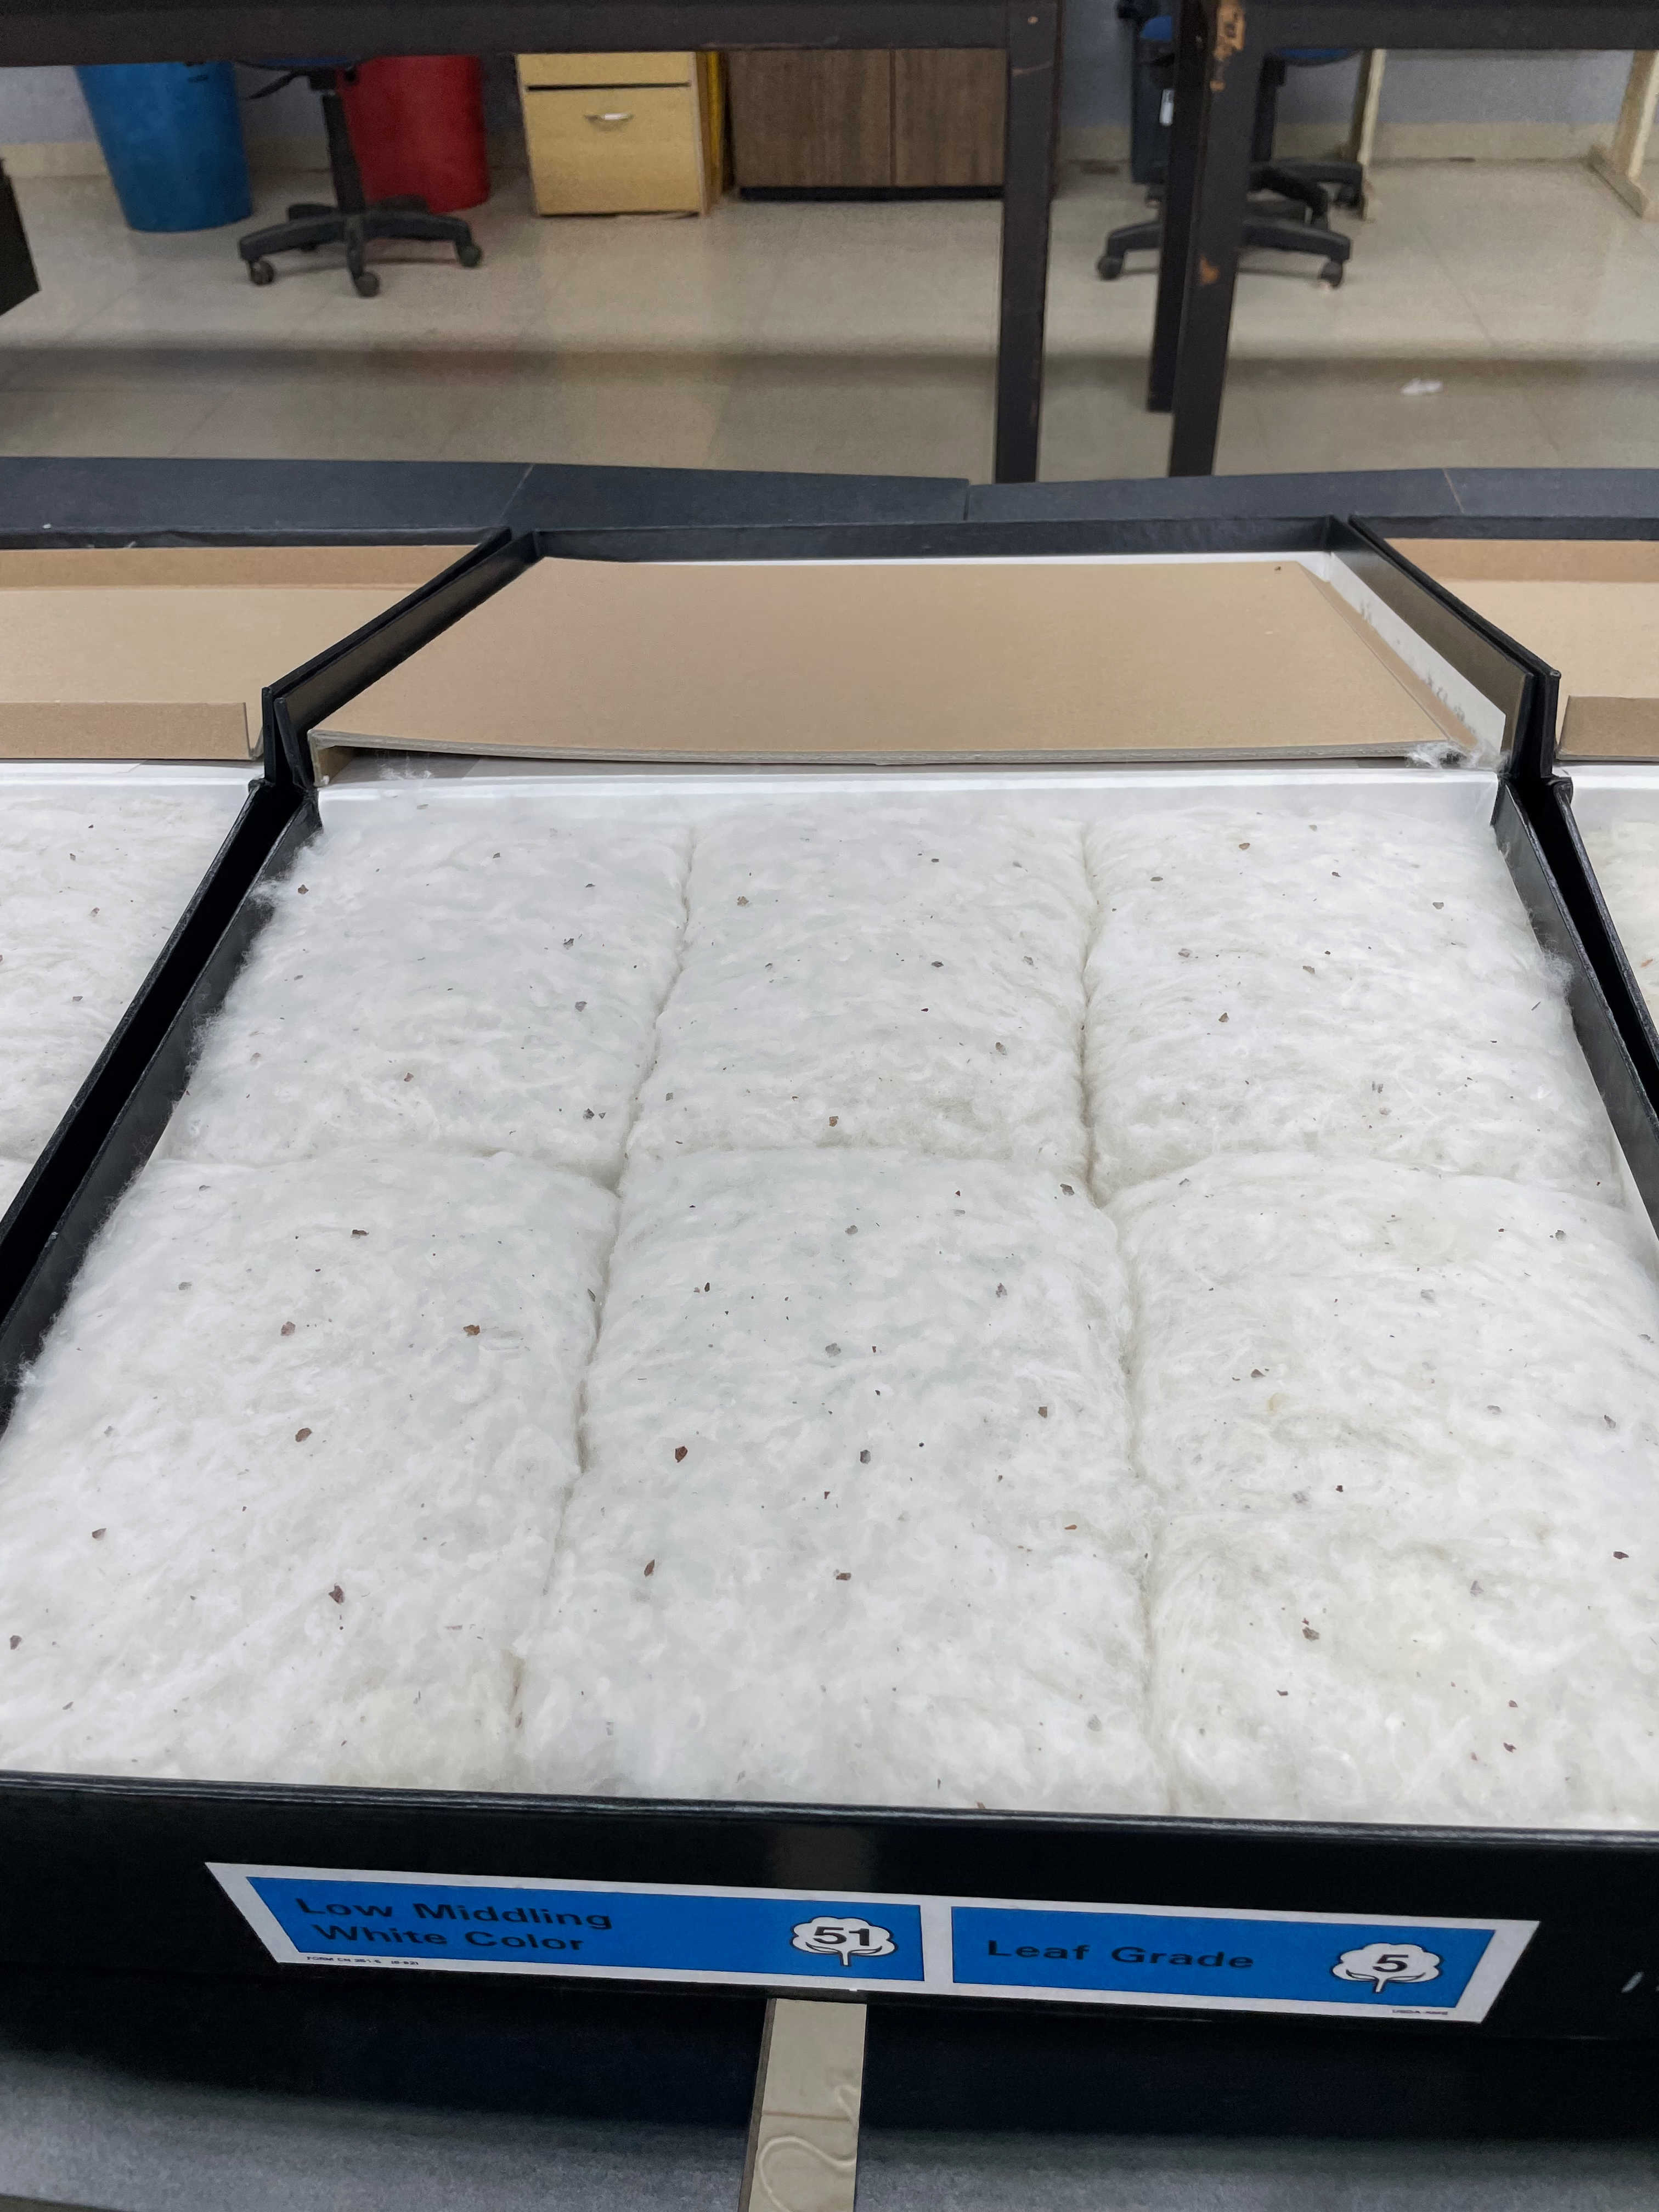
\includegraphics[trim={0 0 0 5cm},clip, scale=.3]{images/padrao_fisico_universal.jpeg}
            \end{center}
            \legend{Fonte: Do Autor}
        \end{figure}

        O protocolo de análise é rigoroso e inicia-se pela calibração visual do técnico, que deve memorizar os padrões físicos antes de iniciar a classificação, podendo consultá-los sempre que necessário para evitar desvios de julgamento. O manuseio da amostra exige técnica específica: ela deve ser subdividida longitudinalmente em camadas, com cuidado para não descaracterizar sua estrutura. As duas faces com maior incidência de defeitos visíveis, são selecionadas e voltadas para cima para a avaliação final.

        Neste exame, o classificador julga simultaneamente múltiplos atributos qualitativos, conforme detalhado por \citeonline{abbade2014agro}:

        \begin{itemize}
            \item \textbf{Cor:} Avaliada pela combinação de matiz, saturação e brilho, sendo categorizada em classes (Branco, Ligeiramente Manchado, Manchado, Tingido e Amarelo);
            \item \textbf{Impurezas (Leaf Grade):} Quantificação visual de cascas, folhas, caules e outras matérias estranhas. O grau é atribuído em uma escala de 1 a 8, na qual 1 representa a amostra mais limpa e 8, a mais suja;
            \item \textbf{Preparação:} Identificação de defeitos oriundos do processo de beneficiamento, como a aspereza e a formação de nós de fibra (emaranhados de fibras);
            \item \textbf{Contaminações:} Presença de materiais não vegetais (plásticos, óleos, entre outros) que desclassificam o lote.
        \end{itemize}

        A determinação final do ``Tipo'' é uma composição entre o padrão de cor e o grau de folha, registrada no Laudo de Classificação (Tabela \ref{tab_tipo_cor}).

        Apesar da padronização dos critérios, a classificação visual possui limitações inerentes à percepção humana. \citeonline{matusiak2010important} argumentam que a análise sensorial é fortemente influenciada por fatores como cansaço visual, experiência do técnico e condições de iluminação. Essa subjetividade gera variabilidade nos resultados, tanto entre diferentes avaliadores quanto nas decisões do mesmo técnico em momentos distintos. Além disso, a dificuldade natural do olho humano em distinguir nuances sutis de cor ou quantificar impurezas milimétricas reforça a necessidade de sistemas de Visão Computacional, que oferecem a reprodutibilidade e a precisão objetiva exigidas pela indústria.

        \afterpage{%
    \clearpage% Flush earlier floats (otherwise order might not be correct)
    \thispagestyle{empty}% empty page style (?)
    \begin{landscape}% Landscape page
        \centering % Center table
        \begin{table}
            \centering
            \caption{Códigos dos tipos de Cor, Classes de Cor ou Grau de Cor do Algodão Upland}
            \begin{tblr}{
                width = \linewidth,
                colspec = {Q[l,m,400]Q[c,m,180]Q[c,m,220]Q[c,m,180]Q[c,m,220]Q[c,m,180]},
                row{1} = {font=\bfseries},
                vline{2-6} = {-}{},
                hline{3-9} = {-}{},
                hline{1-2,10} = {2pt}
              }
                                                                                  & Branco & Ligeiramente Creme & Creme & Avermelhado & Amarelado \\
              Cor Boa Média - GM (Good Middling)                         & 11              & 12                          & 13             & -                    & -                  \\
              Cor Estritamente Média-SM (Strict Middling)                & 21              & 22                          & 23             & 24                   & 25                 \\
              Cor Média-M (Middling)                                     & 31              & 32                          & 33             & 34                   & 35                 \\
              Cor Estritamente Abaixo da Média-SLM (Strict Low Middling) & 41              & 42                          & 43             & 44                   & -                  \\
              Cor Abaixo da Média-LM (Low Middling)                      & 51              & 52                          & 53             & 54                   & -                  \\
              Cor Estritamente Boa Comum-SGO (Strict Good Ordinary)      & 61              & 62                          & 63             & -                    & -                  \\
              Cor Boa Comum-GO (Good Ordinary)                           & 71              & -                           & -              & -                    & -                  \\
              Abaixo de Padrão                                           & 81              & 82                          & 83             & 84                   & 85                 
              \end{tblr}
        \label{tab_tipo_cor}
        \end{table}
    \end{landscape}
    \clearpage
}

    \subsubsection{O Impacto do Viés Subjetivo Humano na Definição do Padrão de Referência (\textit{Ground Truth})}
    \label{sec:vies_humano_gt}

        A qualidade preditiva de qualquer sistema de visão computacional profundo é intrinsecamente
        limitada pela fidelidade do sinal de rotulagem utilizado como padrão de referência
        (\textit{ground truth}). Para além dos fatores já discutidos --- cansaço visual, experiência
        do técnico e condições de iluminação --- a subjetividade da tipagem visual regida pela
        Instrução Normativa nº 24/2016 do MAPA é também influenciada por um viés cognitivo-comercial
        do avaliador, resultando em uma concordância entre classificadores humanos experientes que é
        historicamente instável, tanto entre diferentes avaliadores quanto nas decisões do mesmo
        técnico em momentos distintos \cite{matusiak2010important, fisher2023aiassisted}.

        Uma vez que o conjunto de dados de referência utilizado nesta dissertação foi rotulado a
        partir dos laudos de classificação visual humana da algodoeira parceira em Sapezal, Mato
        Grosso (Seção \ref{sec:conjunto_dados}), as inconsistências inerentes ao julgamento humano
        atuam como um ruído estocástico incorporado aos próprios rótulos de treinamento. Esse fator
        impõe um limite superior (\textit{upper bound}) ao desempenho teórico absoluto das redes
        neurais avaliadas, uma vez que os modelos são forçados a mapear fronteiras de decisão
        qualitativas e fluidas que, por vezes, carecem de consistência física estrita.

        \clearpage

    \subsubsection{A Classificação Instrumental (HVI)}

        Paralelamente à análise visual, a segunda amostra de trabalho é destinada à classificação instrumental. Diferente da avaliação humana, essa etapa exige rigoroso controle ambiental: as amostras devem permanecer em repouso em bandejas teladas por, no mínimo, 24 horas em laboratório climatizado (temperatura e umidade controladas) para atingir o equilíbrio de umidade com o ambiente, garantindo a reprodutibilidade das leituras físicas.

        A análise é realizada em equipamentos de alto volume conhecidos como HVI, calibrados diariamente com padrões internacionais do USDA. A Figura \ref{fig_hvi_maquina} apresenta o modelo Uster HVI 1000, amplamente adotado pela indústria têxtil.

        \begin{figure}[H]
            \caption{\label{fig_hvi_maquina}Equipamento Uster HVI 1000}
            \begin{center}
                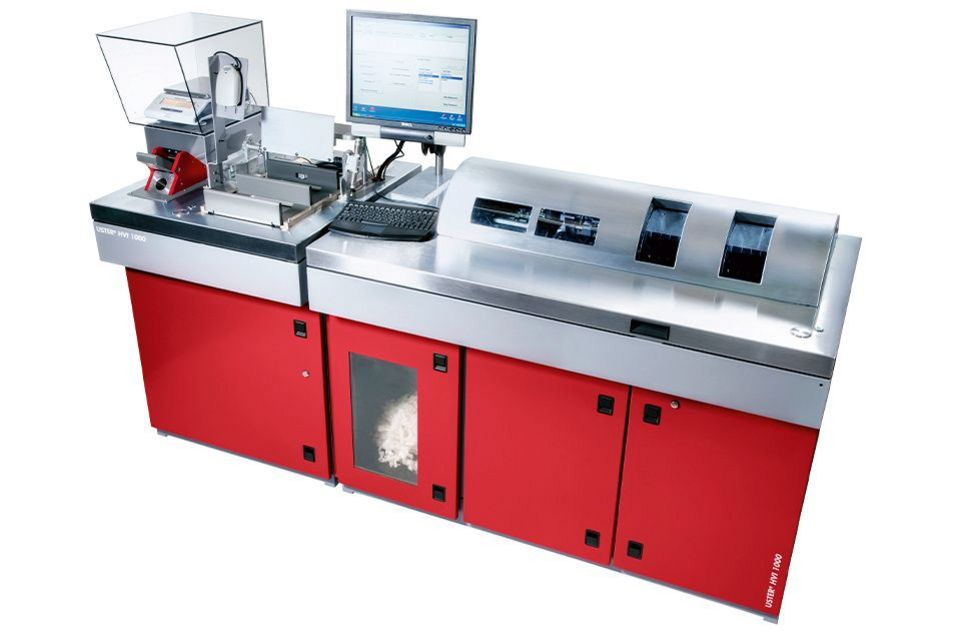
\includegraphics[trim={0 0 0 0},clip, scale=.3]{images/hvi_maquina.jpg}
            \end{center}
            \legend{Fonte: \cite{uster2024hvi}}
        \end{figure}

        O protocolo operacional do HVI automatiza a mensuração de múltiplas propriedades físicas. O teste de \textit{Micronaire} é realizado em um único corpo de prova por meio da compressão de massa de fibras, enquanto os demais parâmetros de comprimento e resistência são obtidos por meio de pentes óticos e garras mecânicas em dois corpos de prova por amostra, gerando uma média do lote.

        Os principais parâmetros fornecidos no laudo técnico são:

        \begin{itemize}
            \item \textbf{Comprimento da Fibra (UHML):} Comprimento médio da metade superior das fibras.
            \item \textbf{Índice de Uniformidade do Comprimento da Fibra (\%UI):} Relação entre o comprimento médio total das fibras e o comprimento médio das fibras mais longas.
            \item \textbf{Resistência ou Tenacidade da Fibra (Str):} Medida da força necessária para romper as fibras, expressa em gf/tex.
            \item \textbf{Alongamento à Rotura da Fibra (\%Elg):} Percentual de extensão que a fibra suporta antes de romper.
            \item \textbf{Micronaire da Fibra (Mic):} Combinação de finura e maturidade da fibra.
            \item \textbf{Grau de Reflectância (\%Rd):} Nível de luminosidade e cor branca refletida pelas fibras.
            \item \textbf{Grau de Amarelamento (+b):} Índice que expressa o nível de amarelamento da fibra.
            \item \textbf{Índice de Fibras Curtas (\%SFI):} Percentual de fibras com comprimento inferior a 0,50 polegadas.
            \item \textbf{Índice de Consistência da Fiação (SCI):} Valor calculado com base nas propriedades físicas das fibras e sua correlação com a performance de fiação.
        \end{itemize}

        Embora o HVI tenha trazido objetividade às transações comerciais, ele apresenta limitações críticas sob a ótica da classificação final. Além do alto custo de aquisição e manutenção \cite{cottonbrazil2021}, o equipamento fornece métricas baseadas em médias globais da amostra. Isso significa que, embora o HVI quantifique com precisão a área total de impurezas, ele não captura a percepção visual holística, como a distribuição espacial da sujeira, a textura e o contraste com a fibra, utilizada pelos classificadores humanos para determinar o ``Tipo'' comercial. Essa lacuna de percepção é justamente o nicho onde sistemas de visão computacional baseados em aprendizado profundo se destacam, pois são capazes de correlacionar padrões visuais complexos diretamente com os graus de qualidade padronizados, oferecendo uma alternativa automatizada e consistente à subjetividade humana.

    \subsubsection{A Relação entre o Visual e o Instrumental}

        A integração entre a subjetividade da análise visual e a objetividade instrumental baseia-se historicamente nos estudos de \citeonline{nickerson1958grade}. Buscando traduzir a percepção humana para grandezas físicas mensuráveis, os autores desenvolveram o colorímetro Nickerson-Hunter, estabelecendo as bases para o atual diagrama de cores utilizado pelo sistema HVI.

        Conforme ilustrado na Figura \ref{fig_hvi_color_chart}, a relação é estabelecida em um plano bidimensional no qual:

        \begin{itemize}
            \item O eixo vertical (\textbf{\%Rd}) representa a \textbf{Reflectância} (brilho), correlacionando-se com a escala de cinzas (do branco ao cinza escuro);
            \item O eixo horizontal (\textbf{+b}) representa o \textbf{Grau de Amarelamento}, indicando a saturação da cor amarela na fibra.
        \end{itemize}

        As interseções desses valores formam clusters que correspondem às classes visuais tradicionais (por exemplo, \textit{Middling}, \textit{Strict Low Middling}). Dessa forma, o HVI consegue converter leituras sensoriais em uma ``nota'' comercial compatível com o julgamento humano.

        \clearpage
        \begin{figure}[H]
            \caption{\label{fig_hvi_color_chart}Diagrama de Cores relacionando parâmetros físicos (\%Rd e +b) com a classificação visual.}
            \begin{center}
                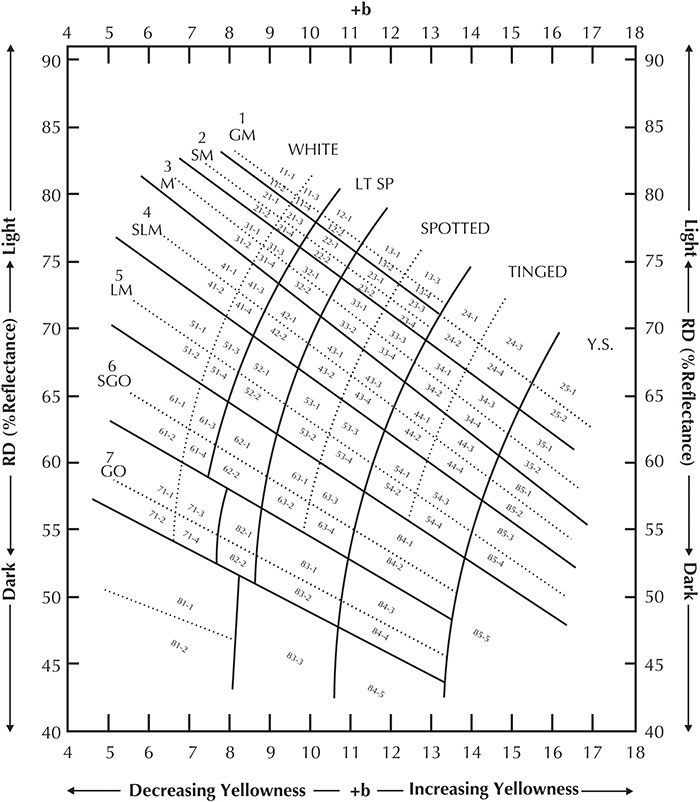
\includegraphics[trim={0 0 0 0},clip, scale=.5]{images/hvi_color_chart.jpg}
            \end{center}
            \legend{Fonte: \citeonline{cottoninc2024hvicolor}}
            % \nota{}
        \end{figure}

        Entretanto, essa correlação robusta observada na análise de cor não se verifica com a mesma eficácia para os parâmetros de impurezas e preparação. Enquanto o HVI mensura a sujeira por contagem de partículas e área ocupada, o classificador humano avalia a aparência geral, considerando o contraste, o tamanho e a natureza do resíduo (folha, casca ou caule). Estudos indicam que a correlação entre o ``Grau de Folha'' visual e a leitura de ``\%Area'' do HVI pode ser baixa em lotes com sujeira heterogênea.

        Essa discrepância evidencia uma lacuna tecnológica: o instrumento é preciso na física (cor), mas limitado na interpretação de padrões complexos (sujeira e textura). É nesse cenário que se insere a proposta desta dissertação: utilizar técnicas de visão computacional para reproduzir a percepção cognitiva humana, buscando uma classificação de qualidade que considere não apenas a estatística da sujeira, mas sua morfologia e distribuição visual na pluma.


\section{Visão Computacional Aplicada à Agricultura}
\label{sec:cv_agricultura}

    Esta seção explora os fundamentos teóricos da visão computacional e dos sistemas de processamento de imagens. A partir de um resgate histórico da disciplina, o texto detalha a arquitetura formal desses sistemas e sua aplicação no agronegócio, com ênfase nas tecnologias e métodos aplicados à cultura do algodão.

    A visão computacional, embora frequentemente associada às inovações recentes da inteligência artificial, possui raízes que remontam a meados do século XX. Segundo a revisão histórica de \citeonline{oliveira2024visao}, a área foi idealizada inicialmente em 1955, sob a premissa de equipar computadores com capacidades sensoriais análogas aos ``olhos e ouvidos'' humanos. Nas décadas seguintes, especialmente nos anos 1970, pesquisadores acreditavam que a emulação da visão biológica seria um marco rapidamente alcançável. Nesse contexto, destaca-se o trabalho seminal de \citeonline{marr1976vision} no campo da neurofisiologia, que propôs uma abordagem computacional para a visão, formulando algoritmos para a interpretação de cenas que serviram como alicerce para grande parte da pesquisa subsequente \cite{vaina2004marr}.

    Contudo, a evolução da área revelou que o processamento visual era intrinsecamente mais complexo do que o previsto, dada a lacuna de conhecimento sobre como o próprio cérebro humano interpreta estímulos visuais. Após décadas de avanços progressivos e o aumento do poder computacional, a visão computacional consolidou-se como a disciplina científica dedicada ao desenvolvimento de métodos que permitem às máquinas não apenas capturar, mas interpretar e ``compreender'' imagens com um nível de abstração semelhante à percepção humana \cite{ballard1982computer}.

    % Revisado
\subsection{Fundamentos de um Sistema de Visão Computacional}

    Um sistema de visão computacional é a integração de \textit{hardware} e \textit{software} projetada para simular a percepção visual humana. \citeonline{saldana2013review} definem que tais sistemas têm o objetivo de extrair e analisar informações de objetos de forma automática, objetiva e não invasiva. A arquitetura típica estrutura-se de três pilares fundamentais: o dispositivo de aquisição de imagens (sensores), o sistema de iluminação e a unidade de processamento (software).

    \subsubsection{Aquisição de imagens}

        A aquisição da imagem é o primeiro estágio do processo, no qual a radiação eletromagnética refletida pelo objeto é convertida em dados digitais. Embora existam sensores baseados em ultrassom, raios-X e espectroscopia no infravermelho próximo (\textit{Near Infrared} --- NIR), as câmeras digitais operando no espectro visível são os dispositivos predominantes na agricultura de precisão \cite{brosnan2004improving}.

        No núcleo dessas câmeras, a captura é realizada por dois tipos principais de sensores: CCD (\textit{Charge-Coupled Device}) e CMOS (\textit{Complementary Metal-Oxide-Semiconductor}).

        As câmeras CCD são historicamente reconhecidas pela alta fidelidade de imagem e sensibilidade em condições de baixa luminosidade. Isso decorre de sua arquitetura, que privilegia uma maior área fotossensível (fator de preenchimento) e uniformidade na resposta dos pixels, resultando em baixo ruído e ampla faixa dinâmica. Tais características as tornaram padrão em aplicações científicas de alta precisão. Contudo, seu alto consumo energético e a complexidade dos circuitos externos limitam sua portabilidade \cite{littwiller2001ccd_cmos}.

        Em contrapartida, a tecnologia CMOS evoluiu drasticamente nas últimas décadas. Sua arquitetura permite a integração de conversores e amplificadores diretamente no pixel, reduzindo o consumo de energia, o tamanho físico e o custo de fabricação. Embora versões antigas apresentassem maior ruído, sensores CMOS modernos atingiram níveis de qualidade comparáveis aos CCDs, tornando-se a escolha dominante para dispositivos móveis e sistemas embarcados no campo \cite{bigas2006cmos}. O Quadro \ref{quad:ccd_vs_cmos} resume as diferenças técnicas entre as tecnologias.

        \begin{table}[ht]
    \centering
    \caption{Resumo comparativos das principais características entre sensores CCD e CMOS}
    \begin{tabular}{l|c|c}
    \hline
    \textbf{Característica}             & \textbf{CCD}                  & \textbf{CMOS}                  \\ \hline
    Consumo de energia                  & Alto                          & Baixo                          \\ 
    Custo                               & Alto                          & Baixo                          \\ 
    Integração em chip                  & Não                           & Sim                            \\ 
    Flexibilidade                       & Limitada                      & Alta                           \\ 
    Faixa dinâmica                      & Alta                          & Limitada                       \\ 
    Sensibilidade                       & Alta                          & Limitada                       \\ 
    Ruído                               & Baixo                         & Alto                           \\ 
    Qualidade de imagem                 & Alta                          & Limitada                       \\ 
    Velocidade                          & Limitada                      & Alta                           \\ 
    Tamanho físico do sistema           & Maior                         & Menor                          \\ 
    Aplicações                          & Alta qualidade, ciências      & Dispositivos móveis, segurança \\ \hline
    \end{tabular}
    \label{tab:ccd_vs_cmos}
    \legend{Fonte: \citeonline{bigas2006cmos}}
\end{table}

        No entanto, para a aplicação específica da classificação de algodão, a escolha do sensor impõe desafios críticos que vão além da arquitetura de fabricação. A natureza física da pluma exige características sensoriais específicas para garantir a correlação com os padrões comerciais:

    \begin{enumerate}
        \item \textbf{Faixa Dinâmica (\textit{Dynamic Range}):} O algodão beneficiado possui alta refletância (brilho), criando um cenário de alto contraste em que as impurezas são significativamente mais escuras que a fibra. \citeonline{li2025measurement} destacam que a captura de imagens nesse cenário enfrenta o desafio de sombras e brilho excessivo; sensores com baixa faixa dinâmica tendem a saturar nos brancos ou perder detalhes nas áreas sombreadas das impurezas, exigindo algoritmos robustos de segmentação (como o Color-Unet) para garantir a consistência da medição de cor.
        
        \item \textbf{Resolução Espacial:} A detecção de impurezas milimétricas impõe um desafio de amostragem. \citeonline{li2025cottonyolo} argumentam que métodos tradicionais falham em detectar esses pequenos objetos devido à complexidade do fundo e à mistura de pixels. O uso de sensores de alta resolução, aliados a redes neurais profundas, torna-se mandatório para distinguir contaminantes minúsculos que, em resoluções menores, seriam invisíveis ou confundidos com ruído.
        
        \item \textbf{Fidelidade de Cor:} A classificação comercial depende estritamente dos parâmetros de Amarelamento (+b) e Reflectância (Rd). Segundo \citeonline{li2023novel}, a simples captura RGB (\textit{Red, Green, Blue}) não garante a correlação com o padrão HVI. É necessária uma calibração rigorosa e a conversão para espaços de cor perceptuais (como CIE $L^*a^*b^*$ ou Hunter) para que o sistema de visão atinja coeficientes de determinação superiores a 0,88 quando comparado aos colorímetros industriais, evitando erros de graduação que resultam em prejuízo financeiro.
    \end{enumerate}


        Além do sensor, a integridade da análise depende do formato de armazenamento. Em aplicações científicas, formatos de compressão sem perdas, como PNG, BMP ou TIFF, são preferíveis, pois preservam o valor exato de cada pixel. Formatos com perdas, como o popular JPEG, utilizam algoritmos que descartam informações de alta frequência para reduzir o tamanho do arquivo. Para a classificação de algodão, na qual a textura fina e a presença de micro-impurezas são críticas, os artefatos de bloco gerados pela compressão JPEG podem ser interpretados erroneamente pelos algoritmos como ruído ou defeitos, comprometendo a precisão do modelo \cite{vanderwalt2014scikit}.


    \subsubsection{Iluminação}

        A iluminação é um componente crítico nos sistemas de visão computacional, pois define as propriedades ópticas de absorção, reflexão e transmissão dos objetos analisados. Uma captura bem iluminada reduz a necessidade de etapas algorítmicas complexas de pré-processamento, aumentando a eficiência computacional e a precisão das análises \cite{chen2002machine_vision}. Segundo \citeonline{zhang2014computer}, a fonte de luz ideal deve fornecer uma incidência uniforme e estável, realçando as características de interesse e mitigando reflexos ou sombras indesejáveis que possam comprometer a segmentação do objeto.

        No contexto específico da classificação de algodão, a iluminação desempenha um papel duplo e, por vezes, antagônico, exigindo um compromisso técnico (\textit{trade-off}):

        \begin{itemize}
            \item \textbf{Para Análise de Cor (Simulação de HVI):} A classificação comercial baseia-se na reflectância (\%Rd) e no amarelamento (+b). \citeonline{rady2025computervision}, ao desenvolverem sistemas de visão para graduação de algodão egípcio, demonstraram que a consistência na classificação de cor exige uma iluminação difusa e homogênea. O uso de luz direcional cria sombras e reflexos na fibra que alteram os valores RGB capturados, impedindo a correlação direta com os padrões físicos universais.
            
            \item \textbf{Para Detecção de Impurezas e Robustez:} Paradoxalmente, a luz difusa que favorece a cor tende a ``suavizar'' a textura, ocultando defeitos tridimensionais. \citeonline{verma2026graphcotton} destacam que a variabilidade de iluminação é um dos principais desafios para a segmentação robusta de capulhos e impurezas em cenários complexos. Para detectar contaminantes que possuem a mesma cor da fibra (como plásticos claros) ou defeitos de preparação (nós de fibra), uma componente de luz direcional ou rasante é fundamental para gerar microssombras que revelam a morfologia do objeto, permitindo que modelos de detecção superem as limitações da simples análise de cor.
        \end{itemize}

        Atualmente, a tecnologia LED (\textit{Light-Emitting Diode}) consolidou-se como padrão para solucionar esse dilema. Sua estabilidade espectral e capacidade de controle rápido permitem o desenvolvimento de sistemas de iluminação híbridos ou multiespectrais, que alternam entre configurações difusas e direcionais para capturar o máximo de informação da amostra em uma única inspeção \cite{cubero2010advances}.

        Dessa forma, o projeto do sistema de iluminação para esta dissertação não buscou apenas a visibilidade, mas a fidelidade fotométrica, garantindo que a imagem digital servisse como um \textit{proxy} confiável tanto para a avaliação cromática quanto para a inspeção morfológica da qualidade.


    \subsubsection{Software}

        O componente de \textit{software} atua como o cérebro do sistema de visão computacional, responsável não apenas por orquestrar o \textit{hardware} de captura e iluminação, mas principalmente por implementar os algoritmos de interpretação visual. Historicamente, o desenvolvimento baseava-se em bibliotecas de processamento de imagem clássico (ou \textit{rule-based}), como o OpenCV (\textit{Open Source Computer Vision Library}). Essas ferramentas exigiam que o engenheiro definisse manualmente os descritores matemáticos para extrair bordas, cores ou formas geométricas \cite{opencv_library}.

        No entanto, o estado da arte na agricultura de precisão sofreu uma mudança de paradigma com a consolidação do aprendizado profundo (\textit{Deep Learning}). Conforme revisado por \citeonline{mustofa2023comprehensive}, o foco do desenvolvimento de \textit{software} migrou da engenharia de características manual (\textit{feature engineering}) para a curadoria de dados e o treinamento de redes neurais convolucionais (\textit{Convolutional Neural Networks} --- CNNs). Nesse novo cenário, o \textit{software} não segue mais regras lógicas rígidas baseadas em limiares de cor, mas aprende padrões complexos a partir de exemplos, exigindo \textit{frameworks} robustos para o treinamento e inferência dos modelos.

        Atualmente, dois ecossistemas dominam o desenvolvimento de \textit{software} para visão agrícola:

        \begin{itemize}
            \item \textbf{\textit{Frameworks} de Treinamento (PyTorch/TensorFlow):} São as plataformas nas quais os modelos são construídos. Uma revisão recente de \citeonline{zhang2025bibliometric} destaca que, embora o TensorFlow tenha sido pioneiro na produção industrial, o PyTorch ganhou predominância na pesquisa agrícola devido à sua flexibilidade e facilidade de \textit{debugging}, permitindo a prototipagem rápida de novas arquiteturas para diversas aplicações.
            
            \item \textbf{Arquiteturas de Detecção (YOLOv8/Transformers):} O \textit{software} moderno implementa arquiteturas pré-treinadas que oferecem o equilíbrio ideal entre velocidade e precisão. \citeonline{jelali2025improvedyolov8} destacam a arquitetura YOLOv8 (\textit{You Only Look Once}, versão 8) como o padrão atual para monitoramento agrícola em tempo real, superando antecessores na detecção de pequenos objetos em cenários não estruturados, o que representa uma característica vital para identificar impurezas minúsculas no algodão.
        \end{itemize}

        Por fim, uma camada crítica do \textit{software} frequentemente negligenciada é a ferramenta de anotação e gestão de dados. Como a performance do modelo depende estritamente da qualidade dos exemplos fornecidos (``Garbage In, Garbage Out''), o uso de plataformas para rotulagem consistente de imagens tornou-se um pré-requisito. \citeonline{yang2025ip} argumentam que a falta de anotações precisas é hoje o maior gargalo para a aplicação de visão computacional no campo, exigindo softwares que facilitem a marcação semântica de defeitos e o aumento de dados para robustecer o modelo contra variações de iluminação.

\subsection{Processamento e Análise de Imagens}

    O processamento e a análise de imagens constituem o núcleo algorítmico dos sistemas de visão, transformando a matriz numérica bruta capturada pelo sensor em informações semânticas para a tomada de decisão. A literatura clássica, consolidada por \citeonline{gonzalez2017digital}, organiza esse fluxo em uma hierarquia de três níveis: baixo, médio e alto nível. Embora a ascensão do aprendizado profundo (\textit{deep learning}) tenha automatizado a transição entre essas etapas, a compreensão dessa estrutura permanece fundamental para o design de sistemas robustos.

    \subsubsection{Processamento de Baixo Nível: Pré-processamento}
    
        O processamento de baixo nível engloba operações nas quais tanto a entrada quanto a saída são imagens. O objetivo primordial é a melhoria da qualidade visual e a restauração de dados para facilitar as etapas subsequentes. Técnicas comuns incluem a correção radiométrica (uniformização da iluminação), a redução de ruído via filtros espaciais e a correção geométrica de distorções da lente.
        
        No contexto moderno de redes neurais, esta etapa evoluiu para incluir o aumento de dados (\textit{data augmentation}) e a normalização estatística. \citeonline{shorten2019survey} destacam que, para aplicações agrícolas onde a variabilidade de campo é alta, aplicar transformações geométricas e de cor nas imagens de treinamento é crucial para evitar o \textit{overfitting} e garantir que o modelo generalize bem para diferentes condições de iluminação.

    \subsubsection{Processamento de Nível Intermediário: Segmentação e Representação}
    
        Nesse estágio, a operação transita de imagens para atributos. A tarefa central é a segmentação, que visa particionar a imagem em regiões de interesse: no caso do algodão, separar a fibra do fundo e isolar as impurezas.
        
        Abordagens tradicionais baseavam-se em limiarização (\textit{thresholding}) e detecção de bordas \cite{sonka1993}. Contudo, \citeonline{li2025cottonyolo} argumentam que métodos clássicos falham na classificação de algodão devido à complexidade da textura: sombras na fibra podem ser confundidas com sujeira, e impurezas claras (como plásticos) não possuem contraste suficiente para uma limiarização simples.
        
        Essa limitação impulsionou a adoção de redes neurais convolucionais (CNNs). Diferentemente da extração manual de atributos (forma, textura, momentos), as CNNs aprendem hierarquicamente as representações necessárias: as primeiras camadas da rede atuam como filtros de borda e textura, enquanto as camadas profundas agem como segmentadores semânticos, identificando padrões complexos que escapam à modelagem matemática tradicional \cite{lecun2015deep}.

    \subsubsection{Processamento de Alto Nível: Interpretação e Classificação}
    
        O nível final envolve a ``compreensão'' da cena, atribuindo significado aos objetos segmentados. Na classificação de qualidade do algodão, isso não significa apenas detectar uma partícula, mas interpretá-la semanticamente: classificar se é uma folha, um caule ou um defeito de preparação (\textit{nep}) e, com base no conjunto, atribuir uma nota global ao fardo (Tipo/Grau).
        
        Enquanto sistemas antigos utilizavam classificadores estatísticos (como SVM ou KNN) sobre vetores de características fixos, os sistemas modernos realizam a classificação de forma integrada. O modelo aprende a correlacionar a distribuição espacial e morfológica das impurezas diretamente com os padrões de qualidade comercial, emulando o processo cognitivo de um classificador humano experiente \cite{pacal2024systematic}.

\subsection{Aplicações da Visão Computacional}

    A aplicação da visão computacional no agronegócio ultrapassou a fase experimental para se tornar uma ferramenta essencial na garantia de qualidade e produtividade. A literatura recente evidencia uma migração das técnicas clássicas de processamento de imagem para abordagens baseadas em aprendizado profundo, capazes de lidar com a variabilidade natural dos produtos agrícolas \cite{patricio2018,tian2020}.
    
    Na sequência, discute-se como essa tecnologia evoluiu do monitoramento de campo para a rigorosa inspeção de qualidade industrial, nicho no qual este trabalho se insere.

    \subsubsection{Monitoramento e Detecção de Padrões em Campo}

        No ambiente de cultivo, a visão computacional é amplamente utilizada para a detecção de anomalias biológicas. \citeonline{ahad2023} e \citeonline{ritharson2023} demonstraram que CNNs podem superar a sensibilidade humana na identificação de doenças, atingindo níveis de acurácia superiores a 98\% em culturas de arroz. A tendência atual é a implementação desses modelos em arquiteturas leves (como YOLOv8) para processamento em tempo real \cite{shwetha2024}.
        
        Essa capacidade de detecção estende-se à cultura do algodão ainda no campo. \citeonline{singh2023}, por exemplo, desenvolveram algoritmos para identificar capulhos maduros em tempo real, buscando a automação da colheita. Embora a detecção em campo esteja avançada, o maior desafio tecnológico reside na etapa seguinte: a avaliação da qualidade do produto colhido.

    \subsubsection{Inspeção de Qualidade e Padronização Pós-Colheita}

        A avaliação de qualidade de produtos agrícolas, historicamente subjetiva, tem sido transformada pela automação visual. Desde os trabalhos pioneiros de \citeonline{Majumdar1999} na classificação de cereais por textura, a tecnologia evoluiu para detectar defeitos sutis, muitas vezes imperceptíveis ao olho humano, em esteiras de alta velocidade. \citeonline{zhu2024} aplicaram técnicas de luz estruturada para identificar danos mecânicos em maçãs, validando o uso de visão computacional para a tipificação comercial.

        No contexto específico da fibra de algodão, a pureza e a cor são os atributos mais críticos. A detecção de contaminantes (\textit{foreign matter}) é um problema clássico revisitado por \citeonline{wang2023}, que implementaram a arquitetura YOLOv5 para distinguir fibras de materiais estranhos (cascas, plásticos) com alta velocidade. A complexidade desta tarefa assemelha-se à detecção de ervas daninhas em campo, na qual a distinção entre o ``alvo'' e o ``fundo'' exige robustez contra variações de iluminação e oclusão \cite{juwono2023, subeesh2022}.
        
        Apesar desses avanços pontuais na detecção de contaminantes, ainda existe uma lacuna na correlação direta entre os padrões visuais aprendidos por máquinas e as classes comerciais manuais (Tipo e Cor) utilizadas na comercialização da pluma, conforme estabelecido pelos Padrões Universais. É nessa intersecção entre a avançada capacidade de detecção de objetos (YOLO/CNNs) e a necessidade de padronização comercial que esta dissertação atua.

\section{Classificação Automatizada do Algodão com Visão Computacional}
\label{sec:classificacao_algodao}

    A classificação da pluma de algodão, historicamente dependente da inspeção manual ou de instrumentos laboratoriais como o HVI, atravessa uma profunda mudança de paradigma impulsionada pela inteligência artificial. A convergência entre processamento de imagem, aprendizado de máquina e tecnologias conectadas (\textit{IoT/Edge Computing}) tem se consolidado como uma solução transformadora para superar as limitações dos métodos tradicionais, que frequentemente exigem mão de obra intensiva, demandam tempo excessivo e estão sujeitos à subjetividade.

    A literatura recente evidencia que a aplicação dessas tecnologias evoluiu substancialmente, expandindo-se do monitoramento agrícola em campo para a automação rigorosa do ``processamento inteligente'' e da inspeção de qualidade na indústria. O uso do aprendizado profundo assumiu um papel dominante nesse cenário, viabilizando a extração de características complexas da fibra que abordagens matemáticas ou estatísticas convencionais não conseguiam modelar com precisão.

    Esta seção explora a trajetória tecnológica dessa automação, abordando desde as limitações físicas dos sensores de captura até a evolução dos modelos preditivos. A discussão abrange a transição do aprendizado de máquina clássico para o atual estado da arte baseado em redes neurais convolucionais e transformers, detalhando como a pesquisa moderna tem solucionado a avaliação automatizada dos três pilares da qualidade comercial do fardo: cor, impurezas (\textit{trash}) e preparação.

    %Revisado
\subsection{Limitações Sensoriais e Multiespectrais}

    Embora câmeras RGB sejam predominantes devido ao baixo custo, a literatura aponta limitações físicas críticas na detecção de certos contaminantes. \citeonline{mustafic2016} demonstraram que materiais como plásticos transparentes e papéis brancos possuem assinaturas visuais quase idênticas à da fibra de algodão no espectro visível, tornando-os virtualmente invisíveis para sensores convencionais. A solução proposta pelos autores envolve o uso de imageamento hiperespectral de fluorescência (UV), capaz de distinguir a composição química de contaminantes não botânicos com precisão superior a 90\%.

    Paralelamente, \citeonline{li2024cottonnet} exploraram o uso de espectroscopia no infravermelho próximo (NIR) combinada com redes neurais (\textit{Cotton-Net}) para estimar o teor de impurezas. Embora o método seja eficaz para determinar a composição química global da amostra, ele carece de informação espacial detalhada para classificar a morfologia dos defeitos, reafirmando a necessidade da visão computacional para a avaliação física do aspecto visual do fardo.

\subsection{O Aprendizado de Máquina e a Variabilidade Intra-Amostra}

    A transição da estatística clássica para o aprendizado de máquina marcou a primeira etapa da automação robusta. \citeonline{fisher2023} investigaram a classificação de algodão egípcio utilizando algoritmos de \textit{Random Forest}, superando abordagens baseadas em Máquinas de Vetores de Suporte (\textit{Support Vector Machines}) e redes neurais artificiais clássicas. Uma contribuição fundamental desse estudo foi a introdução da variância intra-amostra como preditor de qualidade: os autores provaram que a uniformidade da cor ao longo da superfície da amostra é tão determinante para a classificação comercial quanto a média dos valores de reflectância.

    Contudo, a eficácia desses modelos esbarra em um gargalo humano: a qualidade da rotulagem dos dados (\textit{ground truth}). \citeonline{fisher2023aiassisted} alertam que a subjetividade e a fadiga dos classificadores humanos introduzem ruído nos dados de treinamento. Para mitigar o alto custo e a inconsistência da anotação manual, os autores propuseram o uso de aprendizado ativo (\textit{Active Learning}), no qual o sistema solicita intervenção humana apenas para imagens de alta incerteza, reduzindo drasticamente o volume de dados necessários enquanto mantém a acurácia do modelo.

\subsection{Abordagens Contemporâneas de Visão Computacional para o Algodão}

    Atualmente, a fronteira do conhecimento reside na aplicação de CNNs para tarefas de segmentação semântica e detecção de objetos, com foco na correlação direta com os parâmetros do HVI.

    No que tange à análise de cor, o principal desafio é a interferência de sombras e sujeira na leitura dos pixels. \citeonline{li2025measurement} propuseram o método inovador \textit{Color-Unet}. Diferentemente das abordagens que calculam a média de toda a imagem, essa rede realiza a segmentação semântica para isolar a fibra pura, excluindo pixels de impurezas e áreas sombreadas. A medição de cor realizada apenas na máscara de fibra limpa resultou em uma correlação significativamente maior com os valores de referência do HVI.

    Para a detecção de impurezas (\textit{Trash}), a arquitetura YOLO (\textit{You Only Look Once}) estabeleceu-se como padrão. \citeonline{li2025cottonyolo} desenvolveram o modelo \textit{Cotton-YOLO}, uma versão otimizada com módulos de atenção projetados especificamente para detectar impurezas milimétricas que redes genéricas não conseguem identificar. Avançando para a quantificação precisa, \citeonline{jiang2024cottonyoloseg} introduziram o \textit{Cotton-YOLO-Seg}, que não apenas detecta o objeto, mas realiza a segmentação de instância (pixel a pixel). Isso permite o cálculo exato da área ocupada por cada partícula, viabilizando a automação do parâmetro \textit{\% Area} do HVI com precisão inédita.

    Por fim, a avaliação da preparação (irregularidades como nós de fibra) também se beneficia dessas arquiteturas. \citeonline{arachchi2024classification} aplicaram CNNs baseadas em \textit{transfer learning} (como a \textit{Inception V3}) para classificar defeitos em fios de algodão, demonstrando que padrões morfológicos sutis de emaranhamento podem ser aprendidos eficazmente por redes profundas, uma lógica que se estende à avaliação da pluma crua.

\section{Arquiteturas de Aprendizado Profundo para Classificação de Imagens}
\label{sec:arquiteturas}

    A eficácia dos sistemas de visão computacional não está apenas no volume de dados ou no poder de processamento bruto, mas fundamentalmente no \textit{design} das arquiteturas de extração de características. Na classificação da pluma de algodão, o modelo enfrenta um desafio multiescala crônico, exigindo um campo receptivo global para avaliar a uniformidade da cor e a distribuição das fibras, ao mesmo tempo em que necessita de altíssima sensibilidade local para detectar impurezas milimétricas e defeitos de preparação (nós de fibra).

    Historicamente, a superação desses desafios acompanhou a própria evolução das topologias de redes neurais. A transição de redes rasas para modelos ultraprofundos exigiu inovações matemáticas substanciais para lidar com gargalos computacionais e com a degradação do gradiente (\textit{vanishing gradient}). Mais recentemente, a hegemonia das operações puramente convolucionais passou a ser desafiada por mecanismos de autoatenção (\textit{self-attention}) global, redefinindo os limites da representação visual das máquinas.

    Esta seção mapeia a trajetória evolutiva das arquiteturas de estado da arte em classificação de imagens, agrupando-as por seus paradigmas fundamentais de \textit{design}. A análise parte dos blocos construtivos clássicos e da consolidação da profundidade (VGG e Inception), avança pelas soluções de roteamento de gradiente (ResNet e DenseNet), explora os limites da eficiência convolucional (EfficientNet e ConvNeXt) e culmina nos modernos paradigmas baseados em atenção (Vision Transformers e Swin-T). Para cada arquitetura, discute-se não apenas sua inovação teórica, mas principalmente sua viabilidade geométrica e computacional frente à complexidade textural do algodão.

    %Revisado
\subsection{Arquiteturas Fundacionais: VGG e Inception}

    A VGG estabeleceu o uso sistemático de filtros $3 \times 3$, demonstrando que a profundidade é o componente chave para a extração de hierarquias de características. Embora fundamental, sua ineficiência paramétrica e o uso de camadas densas massivas servem hoje como \textit{baseline} histórico. A família Inception introduziu a ideia de processamento multiescala paralelo, capturando texturas em diferentes frequências espaciais, o que pavimentou o caminho para redes com campos receptivos mais inteligentes.

    \subsubsection{A Arquitetura VGG Net}

        A VGG Net, introduzida por \citeonline{vgg2024}, demonstrou que uma rede mais profunda, aliada a uma estrutura uniforme, é o fator determinante para a extração de características em larga escala. Diferentemente de sua predecessora, a \textit{AlexNet}, que utilizava filtros heterogêneos (como $11 \times 11$), a VGG propôs uma filosofia de \textit{design} baseada na simplicidade: a utilização exclusiva de filtros pequenos de $3 \times 3$ empilhados. Matematicamente, uma sequência de três dessas convoluções possui o mesmo campo receptivo efetivo de uma única camada de $7 \times 7$. No entanto, essa abordagem oferece vantagens críticas para a classificação de microtexturas.

        Primeiramente, as três camadas introduzem três funções de ativação ReLU em vez de uma, permitindo que a rede aprenda funções de decisão muito mais complexas e discriminativas. Além disso, enquanto uma camada de $7 \times 7$ com $C$ canais possui $49C^2$ parâmetros, a pilha de três camadas de $3 \times 3$ utiliza apenas $27C^2$ parâmetros. Essa redução de quase 45\% permitiu o aumento da profundidade da rede (até 16 ou 19 camadas) sem um crescimento proibitivo do custo computacional.
        
        Embora existam diversas variantes (de VGG-11 a VGG-19), a VGG-16 tornou-se o padrão para tarefas de visão computacional. Sua estrutura é composta por blocos de camadas convolucionais seguidos por \textit{max-pooling} ($2 \times 2$ com \textit{stride} 2), culminando em camadas totalmente conectadas.

        % \begin{table}[ht]
\centering
\caption{Comparativo Técnico das Arquiteturas VGG Net}
\label{tab:vgg_comparativo}
\begin{tabular}{@{}lccc p{6cm}@{}}
\toprule
\textbf{Modelo} & \textbf{Camadas} & \textbf{Parâmetros} & \textbf{Tamanho (MB)} & \textbf{Diferencial Técnico} \\ \midrule
VGG-11 & 11 & 133M & ~507 & Configuração base; profundidade mínima para convergência. \\
VGG-13 & 13 & 133M & ~508 & Adição de blocos convolucionais duplos no início da rede. \\
VGG-16 & 16 & 138M & ~528 & Equilíbrio ideal entre profundidade e custo; arquitetura SOTA em 2014. \\
VGG-19 & 19 & 144M & ~574 & Máxima capacidade de extração linear; maior custo computacional. \\ \bottomrule
\end{tabular}
\end{table}
        
        Apesar de sua clareza arquitetural, a VGG apresenta limitações em cenários modernos de produção. A dependência de camadas totalmente conectadas massivas resulta em um alto consumo de memória (~528 MB para a VGG-16). Além disso, a ausência de conexões de salto torna o modelo sensível ao desaparecimento do gradiente em profundidades maiores.

        No contexto desta dissertação, a VGG-16 é analisada como um extrator de características robusto. Sua capacidade de capturar microtexturas e sua uniformidade a tornam uma base ideal para \textit{transfer learning}, embora sua eficiência computacional seja inferior a modelos mais recentes como a \textit{EfficientNet}, um ponto crítico para a viabilidade em ambientes agrícolas embarcados.

    \subsubsection{A Arquitetura Inception}

        Enquanto a VGG focava na profundidade linear, a arquitetura Inception (GoogLeNet), introduzida por \citeonline{szegedy2015goingdeeper}, propôs uma mudança arquitetural baseada na esparsidade e na eficiência computacional. O objetivo central era aumentar o poder de representação da rede sem um crescimento paramétrico proibitivo, utilizando para isso o módulo Inception.

        A inovação técnica fundamental da Inception v1 foi o processamento multiescala simultâneo. Em vez de selecionar um tamanho de filtro fixo por camada, o módulo executa convoluções de $1 \times 1$, $3 \times 3$ e $5 \times 5$ em paralelo, concatenando seus resultados. Essa captura multirresolução é altamente vantajosa para a classificação de plumas de algodão: o filtro $3 \times 3$ foca em características locais (fibras individuais e micro-impurezas), enquanto o $5 \times 5$ captura padrões globais (a morfologia geral da amostra). Para viabilizar o custo computacional desse paralelismo, a Inception introduziu convoluções de $1 \times 1$ antes dos filtros maiores para reduzir a profundidade dos canais (\textit{bottleneck}), mantendo a rede leve com 6,8 milhões de parâmetros na v1 (contra 138 milhões da VGG-16).

        As versões subsequentes (v2 e v3) refinaram a arquitetura por meio de princípios de fatoração. Seguindo o objetivo de eficiência matemática, \textit{kernels} grandes ($5 \times 5$) foram substituídos por sequências de $3 \times 3$. Além disso, convoluções quadradas $n \times n$ foram fatoradas em operações assimétricas de $1 \times n$ e $n \times 1$ (ex.: $1 \times 7$ seguido de $7 \times 1$), reduzindo drasticamente as operações em ponto flutuante sem perda de campo receptivo. 

        Esse paradigma de fatoração foi levado ao limite na Xception (\textit{Extreme Inception}) \cite{chollet2017xception}. Essa arquitetura utiliza convoluções separáveis em profundidade (\textit{depthwise separable convolutions}), isolando totalmente a busca por correlações espaciais das correlações entre canais. Dada a sua eficiência paramétrica, consolidou-se como uma das arquiteturas base mais eficazes para tarefas que exigem alta precisão em texturas finas.

        % \begin{table}[ht]
\centering
\caption{Evolução Cronológica e Inovações da Família Inception}
\label{tab:inception_evolution}
\begin{tabular}{@{}ll p{8cm}@{}}
\toprule
\textbf{Versão} & \textbf{Inovação Principal} & \textbf{Impacto Acadêmico / Técnico} \\ \midrule
Inception v1 & Módulo Inception & Introdução do processamento multiescala paralelo e redução de parâmetros. \\
Inception v2 & Batch Normalization & Estabilização do treinamento e aceleração da convergência. \\
Inception v3 & Fatoração Assimétrica & Substituição de filtros $n \times n$ por $1 \times n$ e $n \times 1$; redução de gargalos. \\
Inception v4 & Inception-ResNet & Integração de conexões residuais para treinamento de redes ultra-profundas. \\
Xception & Depthwise Separable & Desacoplamento total de correlações espaciais e de canal; máxima eficiência. \\ \bottomrule
\end{tabular}
\end{table}


\subsection{Conexões Residuais e Densas: ResNet e DenseNet}

    Conforme discutido na seção anterior, avanço na profundidade das redes neurais esbarrou em uma limitação matemática: o problema do desaparecimento do gradiente (\textit{vanishing gradient}). Para solucionar esse gargalo e viabilizar o treinamento de arquiteturas com dezenas ou centenas de camadas, uma nova geração de modelos alterou fundamentalmente o roteamento do fluxo de informações.

    No contexto da classificação de plumas de algodão, essas abordagens tornaram-se essenciais, pois garantem que os detalhes sutis das micro-impurezas não sejam degradados ou perdidos ao longo de um processamento profundo. As subseções a seguir detalham as duas topologias mais influentes dessa fase: a ResNet e a DenseNet.

    \subsubsection{A Arquitetura ResNet}

        A introdução das Redes Residuais (ResNet) por \citeonline{he2016resnet} marcou um ponto de inflexão na visão computacional ao solucionar o problema da degradação em redes ultraprofundas. Antes da ResNet, adicionar camadas a uma CNN resultava em maiores erros de treinamento, devido à dificuldade dos otimizadores em convergir para mapeamentos de identidade em arquiteturas puramente sequenciais.

        Para contornar esse obstáculo, a ResNet fundamenta-se na premissa de que é matematicamente mais eficiente otimizar um resíduo do que um mapeamento direto não referenciado. Em vez de forçar um bloco de camadas a aprender uma função desejada $H(x)$, a arquitetura o restringe a aprender a função residual $F(x)=H(x)-x$. A saída do bloco passa a ser a soma do resíduo com a entrada original, expressa por:
        
        $$H(x)=F(x)+x$$
        
        Essa formulação é materializada na rede por meio de conexões de salto (\textit{skip connections}), atalhos que permitem ao sinal do gradiente fluir pelas camadas sem atenuação. Na classificação de plumas de algodão, em que sutilezas de textura e coloração poderiam ser perdidas por muitas operações de convolução, o caminho de identidade assegura que as características visuais em baixo nível continuem inalteradas até as camadas de decisão.

        A topologia interna da rede adapta-se em função da profundidade desejada, apoiando-se em dois projetos fundamentais de blocos residuais. Para redes de profundidade intermediária (como ResNet-18 e ResNet-34), utiliza-se o bloco básico (\textit{BasicBlock}), composto por duas convoluções de $3 \times 3$, configuração robusta para a extração de texturas em conjuntos de dados de médio porte. Para arquiteturas mais densas (ResNet-50, ResNet-101 e ResNet-152), implementa-se a estrutura de gargalo (\textit{bottleneck}). Esse \textit{design} aplica uma sequência de convoluções de $1 \times 1$, $3 \times 3$ e $1 \times 1$, utilizando as camadas unitárias exclusivamente para redução e subsequente restauração da dimensionalidade dos canais. Essa estratégia de compressão reduz drasticamente o número de parâmetros e as operações em ponto flutuante (GFLOPs), permitindo que modelos como a ResNet-101 apresentem um custo computacional significativamente inferior ao da VGG-16, mesmo possuindo profundidade muito maior.

        % \begin{table}[ht]
\centering
\caption{Especificações Técnicas da Família ResNet}
\label{tab:resnet_specs}
\begin{tabular}{@{}llcc p{5cm}@{}}
\toprule
\textbf{Modelo} & \textbf{Bloco} & \textbf{Parâmetros} & \textbf{GFLOPs} & \textbf{Cenário de Uso} \\ \midrule
ResNet-18 & Basic & 11.7M & 1.8 & Dispositivos móveis e \textit{edge}. \\
ResNet-34 & Basic & 21.8M & 3.6 & \textit{Baselines} de classificação de textura. \\
ResNet-50 & Bottleneck & 25.6M & 3.8 & Padrão industrial para \textit{transfer learning}. \\
ResNet-101 & Bottleneck & 44.5M & 7.6 & Alta precisão em imagens complexas. \\ \bottomrule
\end{tabular}
\end{table}



    \subsubsection{A Arquitetura DenseNet}

        A arquitetura DenseNet (\textit{Densely Connected Convolutional Network}), proposta por \citeonline{huang2017densely}, representa uma evolução estrutural significativa na topologia das redes convolucionais. Enquanto a ResNet utiliza conexões de salto fundamentadas na adição de mapas de características, a DenseNet estabelece que cada camada seja conectada a todas as camadas subsequentes dentro de um bloco denso por meio de operações de concatenação. Matematicamente, se em uma topologia tradicional a camada $l$ recebe apenas a saída da camada imediatamente anterior ($l-1$), na DenseNet ela recebe como entrada todos os mapas de características das camadas precedentes:
        
        $$x_l = H_l([x_0, x_1, \dots, x_{l-1}])$$
        
        onde $[x_0, x_1, \dots, x_{l-1}]$ denota a concatenação das representações extraídas anteriormente.

        Essa abordagem de conectividade densa oferece três vantagens teóricas diretas para a extração de texturas complexas. Primeiro, maximiza o reuso de características (\textit{feature reuse}). Filtros fundamentais aprendidos no início do bloco, como detectores de bordas e fibras individuais, são repassados intactos, evitando que o modelo precise recalcular padrões básicos em camadas mais profundas. Segundo, gera uma alta eficiência paramétrica. Como o conhecimento representacional é acumulado, as camadas individuais da DenseNet podem operar com uma profundidade de canais muito reduzida, resultando em modelos significativamente mais compactos que as ResNets equivalentes. Terceiro, a topologia promove uma supervisão profunda implícita (\textit{implicit deep supervision}): cada camada recebe um sinal de gradiente direto da função de perda primária, o que estabiliza o treinamento e atua como uma proteção adicional contra o desaparecimento do gradiente.

        A dinâmica dimensional dessa arquitetura é regulada por dois componentes. O primeiro é a taxa de crescimento (\textit{growth rate}, denotada por $k$), o hiperparâmetro que define quantos novos mapas de características cada camada adiciona à rede. Mesmo com um $k$ conservador (como $k=32$), a densidade das conexões garante um elevado poder de representação. O segundo componente atua como um mecanismo de controle: as camadas de transição (\textit{transition layers}). Posicionadas entre os blocos densos, essas camadas realizam a compressão de canais via convoluções de $1 \times 1$ e a redução da resolução espacial por meio de operações de \textit{pooling}, contendo a explosão dimensional inerente às sucessivas concatenações.

        Para o escopo desta dissertação, a DenseNet destaca-se por sua robustez geométrica. A literatura demonstra que a conectividade densa atua como um regularizador natural, mitigando o sobreajuste (\textit{overfitting}) em conjuntos de dados restritos onde a variância interclasse é sutil, consolidando-a como uma base arquitetural altamente eficaz para o reconhecimento de texturas orgânicas e fibrosas.

        % \begin{table}[H]
\centering
\caption{Variações da Arquitetura DenseNet-BC e Cenários de Aplicação}
\label{tab:densenet_variacoes}
\begin{tabular}{@{}lccc p{6.5cm}@{}}
\toprule
\textbf{Modelo} & \textbf{Camadas} & \textbf{Parâmetros} & \textbf{GFLOPs} & \textbf{Cenário de Uso Sugerido} \\ \midrule
DenseNet-121 & 121 & 8.0M & 2.8 & \textit{Baseline} para classificação de texturas; ideal para prototipagem rápida e \textit{transfer learning}. \\
DenseNet-169 & 169 & 14.1M & 3.4 & Cenários de média complexidade; equilíbrio entre custo computacional e acurácia. \\
DenseNet-201 & 201 & 20.0M & 4.3 & Padrão para imagens médicas e biológicas; alta capacidade de extração de microtexturas. \\
DenseNet-264 & 264 & 33.3M & 5.8 & Pesquisas de alta precisão; cenários onde o volume de dados permite redes ultra-profundas. \\ \bottomrule
\end{tabular}
\end{table}


\subsection{CNNs Modernas: EfficientNet e ConvNeXt}

    Embora as conexões residuais e densas tenham viabilizado topologias ultraprofundas, o roteamento maciço de características gerou inevitáveis gargalos de memória e ineficiência paramétrica. Para solucionar esse desequilíbrio, a literatura mais recente voltou-se para a otimização estrutural e o ganho de escala.

    A EfficientNet liderou esse movimento ao introduzir o redimensionamento composto (\textit{compound scaling}), equilibrando matematicamente profundidade, largura e resolução. Para a classificação do algodão, essa arquitetura é vital: ela permite o processamento em altíssima resolução, essencial para detectar micro-impurezas, mantendo a viabilidade computacional. Em paralelo, a arquitetura ConvNeXt revisitou e modernizou o \textit{design} puramente convolucional, otimizando proporções de blocos e tamanhos de \textit{kernels} para provar que as CNNs clássicas continuam atingindo o estado da arte. As subseções a seguir detalham a matemática dessas duas abordagens.

    \subsubsection{A Arquitetura EfficientNet}

        A família EfficientNet, introduzida por \citeonline{tan2019efficientnet}, redefiniu o \textit{design} de redes convolucionais ao propor que o aumento da capacidade de um modelo não deve ser arbitrário. Os autores propuserarm o método de escalonamento composto (\textit{compound scaling}), que equilibra simultaneamente a profundidade, a largura e a resolução da rede. Diferentemente de arquiteturas anteriores que escalonavam apenas uma dimensão de forma empírica (como a profundidade na ResNet), a EfficientNet utiliza um coeficiente composto $\phi$ para coordenar o crescimento estruturado. Matematicamente, as dimensões de profundidade ($d$), largura ($w$) e resolução ($r$) são definidas pelas relações $d = \alpha^\phi$, $w = \beta^\phi$ e $r = \gamma^\phi$. Sob a restrição de que $\alpha \cdot \beta^2 \cdot \gamma^2 \approx 2$, o aumento total de operações de ponto flutuante (FLOPs) é restrito a aproximadamente $2^\phi$. No contexto da classificação de algodão, essa formulação garante que, ao aumentar a resolução da imagem para detectar micro-impurezas, a rede automaticamente expanda sua profundidade (para ampliar o campo receptivo) e sua largura (para processar a maior densidade de dados), mantendo a eficiência operacional.

        A topologia base da família, a EfficientNet-B0, foi desenvolvida por meio de algoritmos de busca de arquitetura neural (\textit{Neural Architecture Search} - NAS). Seu bloco fundamental é o gargalo invertido móvel (\textit{Mobile Inverted Bottleneck} - MBConv), que emprega convoluções separáveis em profundidade (\textit{depthwise separable convolutions}) para reduzir drasticamente o número de operações em comparação com convoluções densas. Adicionalmente, o bloco incorpora o mecanismo de compressão e excitação (\textit{Squeeze-and-Excitation} - SE), um módulo de atenção que recalibra dinamicamente a importância de cada canal, permitindo que o modelo isole características discriminativas da fibra. O processamento não linear é garantido pela função de ativação Swish ($f(x) = x \cdot \sigma(x)$), cuja característica suave e não monotônica auxilia na mitigação da degradação de gradientes.

        Apesar de sua eficiência teórica, a primeira geração apresentava limitações de \textit{hardware}. A evolução para a EfficientNetV2 \cite{tan2021efficientnetv2} solucionou esses gargalos focando na velocidade de treinamento. Nas camadas iniciais, onde a convolução \textit{depthwise} subutiliza a arquitetura dos aceleradores modernos (GPUs), a versão V2 introduz o bloco Fused-MBConv. Essa estrutura funde a expansão de $1 \times 1$ e a convolução de $3 \times 3$ em uma única operação convolucional padrão de $3 \times 3$. Essa alteração resulta em convergência até 11 vezes mais rápida e em modelos parametricamente menores, consolidando a rede como uma solução de altíssimo desempenho.

        % \input{tables/tab_efficientnet}

    \subsubsection{A Arquitetura ConvNeXt}

        A arquitetura ConvNeXt, proposta por \citeonline{liu2022convnext}, surgiu como uma resposta direta à ascensão dos \textit{Vision Transformers} (ViTs). O objetivo do projeto foi investigar se a superioridade dos modelos baseados em atenção residia intrinsecamente no paradigma de autoatenção ou em avanços de \textit{design} macroarquitetural. Por meio de um processo metódico de modernização de uma ResNet padrão, os autores demonstraram que redes puramente convolucionais, quando desenhadas com heurísticas contemporâneas, ainda podem superar os \textit{Transformers} em precisão e eficiência.

        A ConvNeXt integra esses princípios de arquitetura em uma topologia convolucional por meio de alterações fundamentais. No macro \textit{design}, a rede substitui o bloco inicial (\textit{stem}) de processamento pesado por uma camada fragmentadora não sobreposta (\textit{patchify}), operada por uma convolução de $4 \times 4$ com \textit{stride} 4. Além de ajustar a distribuição de blocos por estágio para emular a hierarquia de \textit{Transformers} modernos, a arquitetura adota a estrutura de gargalo invertido (\textit{inverted bottleneck}). Essa topologia expande a dimensão oculta, permitindo que as convoluções espaciais operem em uma dimensionalidade maior antes da projeção final de canais. Aliado a isso, o campo receptivo foi significativamente ampliado com a substituição dos filtros tradicionais de $3 \times 3$ por \textit{kernels} de $7 \times 7$. Para o escopo do algodão, esse campo receptivo extenso é de suma importância: ele permite capturar a continuidade geométrica de fibras longas e mapear a morfologia de impurezas maiores dispersas na pluma.

        No nível do micro \textit{design}, a rede simplifica componentes internos para otimizar o fluxo de gradiente e a estabilidade. As funções de ativação e normalização foram atualizadas e aplicadas de forma esparsa: a tradicional ReLU foi substituída pela função GELU (\textit{Gaussian Error Linear Unit}), e a \textit{Batch Normalization} deu lugar à \textit{Layer Normalization}, utilizadas apenas uma vez por bloco para reduzir a redundância computacional. Na evolução para a ConvNeXt V2 \cite{woo2023convnext}, introduziu-se a camada de Normalização de Resposta Global (\textit{Global Response Normalization} - GRN). Esse mecanismo foi projetado para evitar o colapso de características (\textit{feature collapse}), um problema crônico em treinamentos autossupervisionados, aumentando a competição entre os canais e garantindo que cada filtro aprenda características estritamente únicas da textura do algodão.

        % \begin{table}[ht]
\centering
\caption{Comparativo de Performance e Eficiência: ConvNeXt vs. Swin Transformer}
\label{tab:convnext_vs_swin}
\begin{tabular}{@{}lcccc@{}}
\toprule
\textbf{Arquitetura} & \textbf{Modelo} & \textbf{Parâmetros} & \textbf{FLOPs} & \textbf{Acurácia (IN-1K)} \\ \midrule
Transformer & Swin-T & 28M & 4,5G & 81,3\% \\
Convolucional & \textbf{ConvNeXt-T} & 28M & 4,5G & \textbf{82,1\%} \\ \midrule
Transformer & Swin-B & 88M & 15,4G & 83,5\% \\
Convolucional & \textbf{ConvNeXt-B} & 89M & 15,4G & \textbf{83,8\%} \\ \bottomrule
\end{tabular}
\end{table}

\subsection{Mecanismos de atenção: ViT e Swin Transformer}

    O limite da engenharia baseada em convoluções abriu espaço para um paradigma radicalmente diferente na extração de características: os mecanismos de autoatenção (\textit{self-attention}). Em vez de processar a imagem por meio de varreduras locais de \textit{pixels}, essa nova geração de modelos analisa a informação globalmente, estabelecendo correlações diretas e simultâneas entre todas as partes da amostra. As subseções a seguir detalham a arquitetura pioneira desse movimento, o \textit{Vision Transformer} (ViT), e a sua evolução hierárquica para o processamento de alta resolução, o \textit{Swin Transformer}.

    \subsubsection{A Arquitetura ViT}

        A introdução do \textit{Vision Transformer} (ViT) por \citeonline{dosovitskiy2021vit} desafiou a soberania das redes convolucionais ao transpor a arquitetura \textit{Transformer}, originalmente projetada para o processamento de linguagem natural (PLN), para o domínio da visão computacional. A premissa fundamental da topologia é tratar uma imagem não como uma grade contínua de \textit{pixels}, mas como uma sequência de \textit{tokens} visuais. Para isso, a imagem original é particionada em uma grade de \textit{patches} não sobrepostos, tipicamente com resolução de $16 \times 16$ \textit{pixels}. Cada \textit{patch} é achatado e mapeado para um espaço latente unidimensional por meio de uma projeção linear.

        Como a arquitetura \textit{Transformer} processa os \textit{tokens} em paralelo e carece de um viés indutivo (\textit{inductive bias}) espacial nativo, vetores de posição (\textit{positional embeddings}) são adicionados às projeções para preservar o arranjo geométrico original. O processamento subsequente é regido pelo mecanismo de autoatenção global (\textit{global self-attention}). Diferentemente das operações convolucionais, cujo campo receptivo é inicialmente restrito às dimensões do filtro, a autoatenção permite que cada fragmento interaja matematicamente com todos os outros desde a primeira camada. No contexto da classificação, essa característica confere ao modelo a capacidade de correlacionar fibras situadas em extremidades opostas da amostra, capturando uma representação semântica global que define a qualidade da pluma de algodão.

        Apesar de seu alto poder de representação, o ViT atua como um modelo de propósito geral, desprovido das premissas matemáticas de localidade e invariância à translação inerentes às CNNs. Consequentemente, quando treinado a partir do zero em conjuntos de dados restritos, o modelo tende a apresentar desempenho inferior às redes convolucionais devido à ausência de noções inatas sobre a vizinhança dos \textit{pixels}. Contudo, ao ser pré-treinado em volumes massivos de dados, sua capacidade de generalização suplanta a das arquiteturas tradicionais. Para a aplicação no escopo desta dissertação, em que o conjunto de imagens de plumas de algodão é naturalmente limitado, a utilização do ViT torna-se estritamente dependente de técnicas de \textit{transfer learning}, permitindo que o modelo herde a compreensão espacial universal obtida nos pré-treinos.

        % \begin{table}[ht]
\centering
\caption{Comparativo de Paradigmas: CNN vs. Vision Transformer (ViT)}
\label{tab:cnn_vs_vit}
\begin{tabular}{@{}lll@{}}
\toprule
\textbf{Característica} & \textbf{Convolucionais (CNN)} & \textbf{Vision Transformer (ViT)} \\ \midrule
Unidade de Processamento & Janelas locais (Pixels) & Patches de imagem (Tokens) \\
Campo Receptivo & Cresce com a profundidade & Global desde a primeira camada \\
Viés Indutivo & Localidade e Translação (Fortes) & Fraco (Aprendido via dados) \\
Complexidade Espacial & Linear $O(N)$ & Quadrática $O(N^2)$ \\
Escalabilidade & Satura em grandes datasets & Melhora com o aumento de dados \\ \bottomrule
\end{tabular}
\end{table}

    \subsubsection{A Arquitetura Swin-T}

        A arquitetura \textit{Swin Transformer} (\textit{Shifted Window Transformer}), proposta por \citeonline{liu2021swin}, solucionou as duas principais limitações do ViT original: a complexidade computacional quadrática e a ausência de uma estrutura multiescala. Para isso, a topologia reintroduziu o conceito de pirâmide de características (\textit{feature pyramid}), um pilar clássico das redes convolucionais, no paradigma da autoatenção. Diferentemente do ViT, que mantém uma resolução isotrópica e imutável em toda a rede, o \textit{Swin} emprega camadas de fusão de fragmentos (\textit{patch merging}) para reduzir progressivamente a resolução espacial enquanto aumenta a profundidade dimensional dos canais.

        Para contornar o gargalo computacional, o modelo particiona a imagem em janelas locais não sobrepostas (por exemplo, contendo $7 \times 7$ \textit{patches}) e restringe o cálculo da autoatenção exclusivamente ao interior dessas regiões. Essa estratégia reduz a complexidade assintótica de $O(N^2)$ para $O(N)$, viabilizando o processamento de imagens em altíssima definição. Contudo, para evitar que a rede fique limitada a visões isoladas e perca a coerência global, a arquitetura introduz o mecanismo de Atenção Multicabeça com Janelas Deslocadas (\textit{Shifted Window Multi-Head Self-Attention} - SW-MSA).

        Esse mecanismo opera alternando entre um particionamento de grade regular e um particionamento deslocado nas camadas consecutivas. O deslocamento espacial da grade introduz conexões transversais matemáticas entre \textit{patches} que pertenciam a janelas distintas na iteração anterior. No escopo da classificação de plumas de algodão, essa dinâmica é fundamental: ela permite que o modelo correlacione fibras contínuas ou micro-impurezas que cruzam as fronteiras artificiais das janelas. Dessa forma, o \textit{Swin Transformer} garante uma compreensão estrutural ininterrupta da amostra, aliando a eficiência de memória das hierarquias convolucionais à expressividade superior da atenção global.

        % \begin{table}[H]
\centering
\caption{Especificações Técnicas e Aplicações das Variantes Swin Transformer}
\label{tab:swin_variations}
\begin{tabular}{@{}lccc p{6cm}@{}}
\toprule
\textbf{Modelo} & \textbf{Parâmetros} & \textbf{GFLOPs} & \textbf{Top-1 Acc*} & \textbf{Cenário de Uso na Classificação de Algodão} \\ \midrule
Swin-T (Tiny) & 28M & 4,5 & 81,3\% & Classificação em dispositivos de borda ou triagem preliminar de amostras. \\
Swin-S (Small) & 50M & 8,7 & 83,0\% & Equilíbrio entre custo e precisão para monitoramento de linha de produção. \\
Swin-B (Base) & 88M & 15,4 & 83,5\% & Padrão para pesquisa acadêmica; alta capacidade de distinção entre classes similares. \\
Swin-L (Large) & 197M & 34,5 & 87,3\%** & Máximo desempenho para análise laboratorial de granulação fina (\textit{fine-grained}). \\ \midrule
SwinV2-G (Giant) & 3B & 650+ & 90,1\% & Modelos de fundação; voltado para \textit{benchmarking} e pré-treino massivo. \\ \bottomrule
\end{tabular}
\footnotesize{*Acurácia medida no ImageNet-1K. **Treinado com ImageNet-22K.}
\end{table}



\section{Síntese da Literatura e Lacunas da Pesquisa}

    %Revisado

A revisão bibliográfica apresentada neste capítulo evidencia que a classificação da qualidade da pluma de algodão representa um gargalo crítico na cadeia produtiva. Historicamente dependente da avaliação humana subjetiva ou de instrumentos laboratoriais de alto custo, como o HVI, o setor encontra na Visão Computacional e no Aprendizado Profundo as soluções tecnológicas mais viáveis para a automação objetiva e em larga escala.

O estado da arte revela uma transição clara nas abordagens de extração de características visuais. A trajetória das CNNs, culminando em arquiteturas modernas como EfficientNet e ConvNeXt, estabeleceu um patamar elevado de eficiência e robustez. Essas arquiteturas provaram ser particularmente eficazes na extração de microtexturas e na detecção de impurezas, características fundamentais para a análise de fibras orgânicas. Por outro lado, a ascensão dos modelos baseados em atenção, representados pelo ViT e pelo Swin Transformer, introduziu a capacidade de modelar dependências globais na imagem, permitindo uma análise estrutural que antes era limitada pelo campo receptivo fixo das convoluções. 

% A literatura converge para a premissa de que o desempenho superior em tarefas de classificação industrial não advém apenas da topologia da rede, mas da simbiose entre arquitetura, técnicas de \textit{transfer learning} e receitas modernas de treinamento — incluindo otimizadores desacoplados (como AdamW) e técnicas de regularização.

Apesar da consolidação dessas tecnologias em domínios genéricos de visão computacional, a literatura focada especificamente na classificação automatizada da pluma de algodão ainda é escassa. A ausência de uma comparação sistemática e direta entre as arquiteturas convolucionais modernas e os \textit{transformers} hierárquicos neste contexto agroindustrial revela as seguintes lacunas de pesquisa, as quais justificam o desenvolvimento desta dissertação:

\begin{itemize}
    \item \textbf{Escassez de Dados em Domínios Específicos e Dependência de Pré-treino:} A maioria dos estudos que validam a superioridade dos \textit{Vision Transformers} assume a disponibilidade de conjuntos de dados massivos. A eficácia e a capacidade de convergência dessas arquiteturas em conjuntos de dados restritos de pluma de algodão, onde a anotação de especialistas é custosa e escassa, ainda carecem de validação profunda.
    
    \item \textbf{Similaridade Inter-classes Extrema:} A distinção entre as classes comerciais de pluma envolve variações sutis e a identificação de defeitos milimétricos (como nós de fibra). A literatura atual não explorou exaustivamente como os diferentes mecanismos de extração (convolução local \textit{vs.} atenção global) lidam com a confusão entre classes vizinhas no espectro de qualidade, caracterizando este problema como um autêntico desafio de classificação.
    
    \item \textbf{Robustez sob Condições Operacionais Reais:} A literatura frequentemente avalia modelos em condições laboratoriais altamente controladas. Há uma lacuna significativa quanto à resiliência de arquiteturas estado da arte frente às variações de iluminação, presença de sombras e heterogeneidade na preparação da amostra, fatores típicos da esteira de processamento de algodão.
    
    \item \textbf{\textit{Trade-off} entre Acurácia e Latência para \textit{Edge Computing}:} Embora modelos como a EfficientNet ofereçam eficiência teórica, o impacto real do custo computacional de mecanismos de autoatenção (Swin) na latência de inferência é pouco documentado na área agrícola. Para que sistemas de classificação operem em tempo real no setor produtivo (\textit{Edge Computing}), é imperativo estabelecer \textit{benchmarks} que comparem não apenas o F1-Score, mas o custo paramétrico e a velocidade de inferência (FLOPs) em \textit{hardwares} limitados.
\end{itemize}

Em suma, esta pesquisa propõe-se a preencher essas lacunas ao avaliar, de forma inédita e comparativa, o desempenho das principais arquiteturas de \textit{deep learning} aplicadas à classificação do algodão. O objetivo final é fornecer uma análise empírica robusta que subsidie decisões técnicas no setor produtivo, buscando o equilíbrio ótimo entre o rigor acadêmico da classificação de alta complexidade e a viabilidade técnica de implementação industrial.




\chapter{Metodologia}
\label{chapter:metodologia}
%Revisando

Este capítulo detalha os procedimentos metodológicos e as ferramentas desenvolvidas para a aquisição e o processamento de dados, que constituem a base para o treinamento e a validação do sistema de visão computacional proposto. O \textit{pipeline} sistemático desenvolvido nesta pesquisa é estruturado em quatro etapas consecutivas, integrando os universos de engenharia de \textit{hardware} e \textit{software}: (i) \textbf{Aquisição física}: captura estandardizada das amostras de algodão em pluma utilizando a cabine fotométrica autoral sob dupla temperatura de cor; (ii) \textbf{Pré-processamento visual}: segmentação semântica robusta de fundo via BiRefNet e eliminação cromática no espaço HSV; (iii) \textbf{Engenharia de dados (recorte em blocos)}: extração geométrica da Região de Interesse (ROI) via algoritmo do Maior Retângulo Interno (LIR) e fragmentação estratificada em blocos de $256 \times 256$ pixels; e (iv) \textbf{Modelagem profunda}: processamento, treinamento bayesiano e classificação preditiva por meio das 17 arquiteturas neurais de estado da arte avaliadas. Estas quatro etapas conceituais desdobram-se nas sete seções deste capítulo: as Seções \ref{sec:sistema_aquisicao} e \ref{sec:protocolo_coleta} detalham a aquisição física; a Seção \ref{sec:prepdados} cobre o pré-processamento visual e a engenharia de dados; a Seção \ref{sec:conjunto_dados} descreve a construção do conjunto de dados; e as Seções \ref{sec:modelos}, \ref{sec:ambiente_treinamento} e \ref{sec:desenho_experimental} detalham a modelagem profunda e o desenho experimental. Cada etapa foi projetada com foco na robustez da luminosidade, na padronização das amostras e na reprodutibilidade dos resultados.


\section{Desenvolvimento do Equipamento de Coleta de Imagens}
\label{sec:sistema_aquisicao}

    %Revisado

A estrutura física consiste em uma cabine retangular fechada, construída em MDF, com dimensões de $40 \times 40 \times 60$ cm (largura, profundidade e altura). O materia, de cor branca e opaca, possui o duplo objetivo de bloquear a luz externa e evitar a contaminação colorimétrica por reflexos das paredes. O equipamento possui um compartimento superior isolado para acomodar as fontes de alimentação e a eletrônica, garantindo que a área inferior de captura fique livre de cabos e sombras indesejadas. O dispositivo de captura foi montado centralizado no teto da estrutura, a uma distância focal aproximada de 40 cm da base onde as amostras são introduzidas (através de uma abertura frontal), garantindo um enquadramento constante. Um esquema técnico detalhado do equipamento é apresentado na Figura \ref{fig:caixa}.

O sistema de iluminação foi projetado estrategicamente para lidar com os desafios ópticos da pluma de algodão. Utilizaram-se duas matrizes de fitas de LED de alta intensidade (2000 lm/m) posicionadas na parte superior, fornecendo luz difusa para minimizar a geração de sombras profundas e brilhos especulares na fibra. O sistema permite a alternância de temperaturas de cor: LEDs de 2800K (luz ``quente'') foram empregados para realçar a reflectância e o amarelamento natural da fibra (+b), enquanto LEDs de 6000K (luz ``fria'', próxima à luz do dia) maximizaram o contraste morfólogico das impurezas superficiais. O protocolo de captura gerou três imagens por amostra: apenas 2800K, apenas 6000K, e ambas simultaneamente, compondo um \textit{dataset} multiespectral robusto para o treinamento das redes.

O módulo de aquisição baseou-se em um sensor CMOS operando a uma resolução de $1280 \times 720$ \textit{pixels}. Optou-se por esta tecnologia devido à sua alta viabilidade de implantação em esteiras industriais, unindo baixo custo e baixo consumo energético, conforme fundamentado na revisão de literatura. O sensor foi acoplado a uma lente grande-angular com campo de visão de 140°, o que permitiu maximizar a área de amostragem do algodão capturada na base do equipamento sem a necessidade de elevar a altura da caixa. As distorções geométricas inerentes a lentes de grande angulação foram mitigadas pelo posicionamento centralizado da amostra.


\begin{figure}[H]
\centering
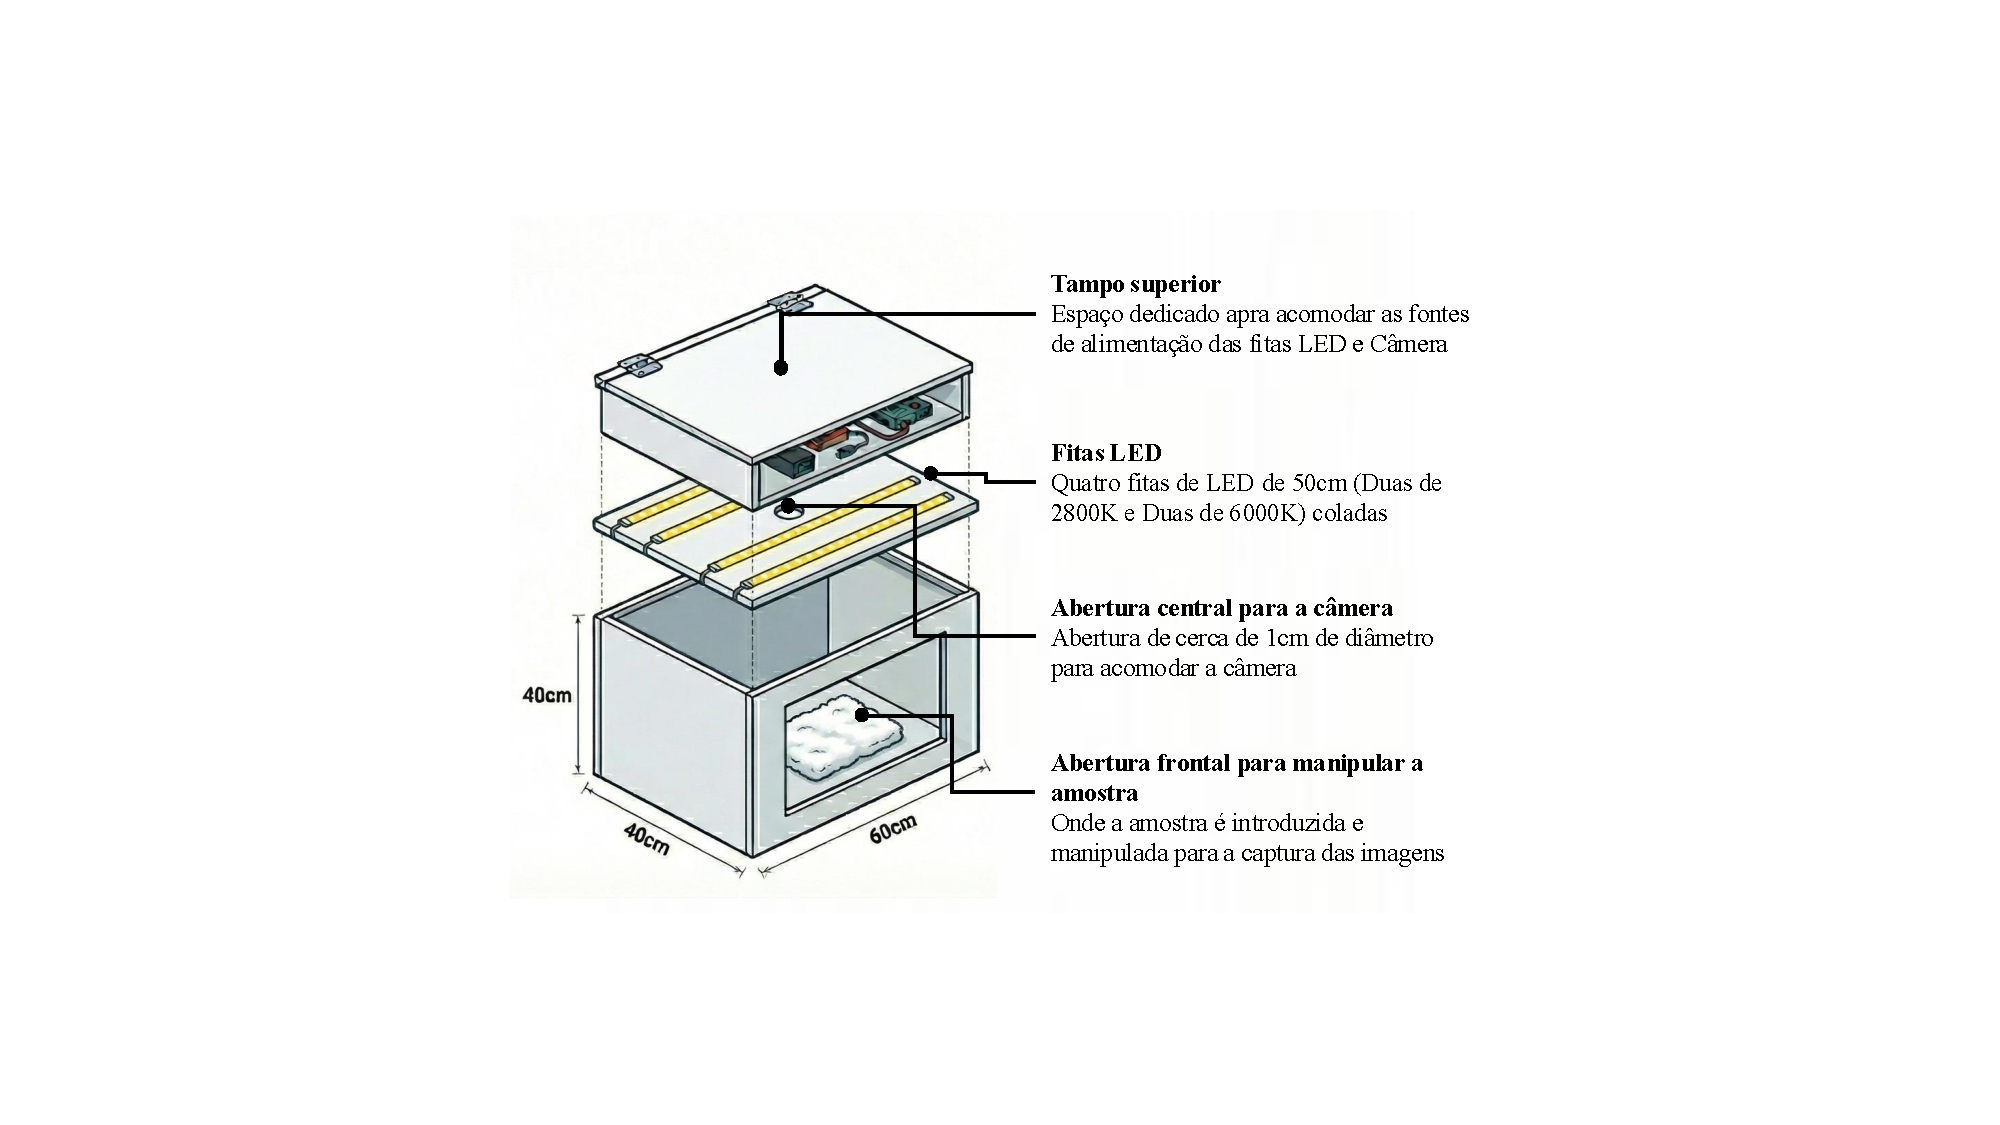
\includegraphics[trim=7.5cm 4cm 7.5cm 4cm, clip, scale=0.9]{images/img_caixa_3.pdf}
% \vspace{-1cm}
\caption{Equipamento de coleta de amostras}
\label{fig:caixa}
\end{figure}

\section{Protocolo de Coleta e Amostragem}
\label{sec:protocolo_coleta}

    %Revisado

O processo de aquisição de dados foi conduzido em ambiente industrial, diretamente nas instalações de uma unidade de beneficiamento de algodão (algodoeira) localizada no município de Sapezal, Mato Grosso, um dos principais polos produtivos do cerrado brasileiro. A coleta ocorreu durante o beneficiamento safra de 2023/2024, totalizando 3.852 imagens brutas, sendo 1.284 para cada uma das três configurações de iluminação (2800K, 6000K e ambas).
    
Para garantir a rastreabilidade e a reprodutibilidade do experimento, estabeleceu-se um protocolo padronizado de captura, desenhado não apenas para gerar as imagens, mas para assegurar o vínculo exato com os laudos de qualidade oficiais (o \textit{ground truth} dos modelos). O fluxo de trabalho operacionalizou-se nas seguintes etapas, ilustradas no fluxograma da Figura \ref{fig:fluxograma_coleta}\footnote{Um vídeo demonstrativo da operação do sistema de captura na unidade de beneficiamento pode ser acessado no Material Suplementar ou por meio do link: \url{https://www.youtube.com/shorts/d_1C78sa11c}}:

\begin{enumerate}
    \item \textbf{Identificação e Rastreabilidade:} O operador inicia o ciclo utilizando um leitor de código de barras para escanear a etiqueta universal da amostra. Ess procedimento vincula automaticamente o ID único do fardo, o lote de processamento e a origem da pluma aos metadados dos arquivos de imagem que serão gerados, eliminando o risco de erros de digitação e garantindo o cruzamento futuro com os dados de classificação oficial (HVI/Visual).
    
    \item \textbf{Posicionamento Padronizado:} A porção de algodão é extraída de sua embalagem e alocada no centro da base do equipamento de captura. O operador realiza a padronização manual do formato da amostra, acomodando a superfície da pluma para garantir a máxima planicidade possível. Esse rigor na modelagem física da amostra é crucial para evitar oclusões severas, minimizar a formação de sombras irregulares e assegurar que a área exposta à lente seja representativa da densidade real do fardo.
    
    \item \textbf{Captura Multiespectral:} Por meio da interface do \textit{software} de controle, a sequência de aquisição é disparada. O operador orquestra manualmente o acionamento dos LEDs e a captura das imagens em três condições sequenciais: iluminação exclusiva de 2800K (AM), iluminação exclusiva de 6000K (BR) e iluminação combinada (AB). As três matrizes de pixels resultantes são armazenadas em um diretório em formato sem perdas (PNG) e atreladas ao ID escaneado no Passo 1.

    \item \textbf{Encaminhamento para Classificação Oficial:} Concluída a aquisição visual, a amostra física é imediatamente reconduzida ao fluxo normal da algodoeira, sendo destinada ao laboratório para a classificação comercial humana. Esse passo é o que permite a rotulagem supervisionada do conjunto de dados nas etapas posteriores da pesquisa.
\end{enumerate}


\begin{figure}[ht!]
\centering
\caption{Fluxograma do processo de coleta de amostras e aquisição de imagens.}
% --- Definição dos estilos dos elementos do fluxograma ---
%   \tikzset{
%     process/.style    = {rectangle, rounded corners, draw, fill=blue!10, text width=7.5em, text centered, minimum height=2em, node distance=1.5cm},
%     startstop/.style  = {circle, draw, fill=green!20, text centered, minimum height=2em, node distance=0.5cm},
%     arrow/.style      = {-{Stealth[]}, thick}
%   }
% --- Desenho do fluxograma ---
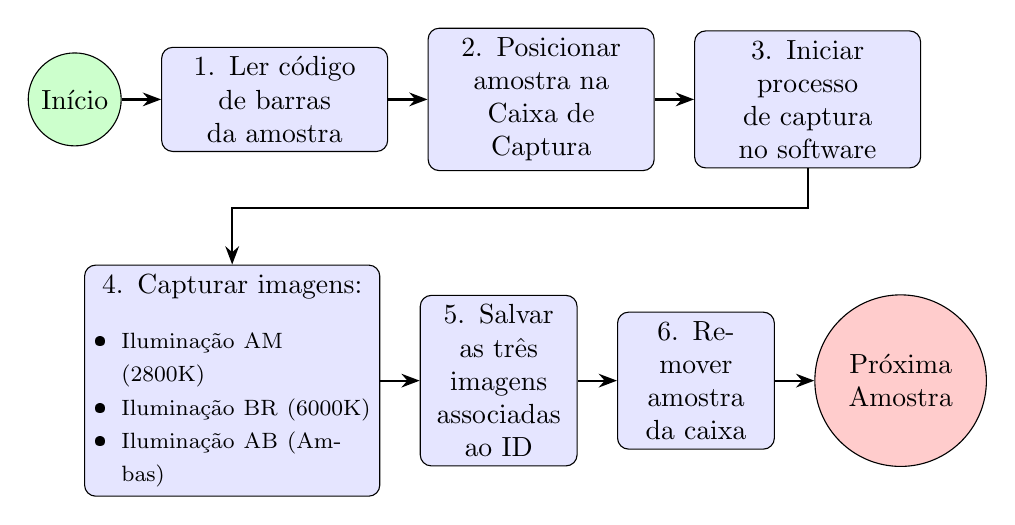
\begin{tikzpicture}[node distance=2cm and 1cm]
    % --- Linha 1 ---
    \node (inicio) [startstop] {Início};
    \node (ler_barcode) [process, right=0.5cm of inicio] {1. Ler código de barras da amostra};
    \node (posicionar) [process, right=0.5cm of ler_barcode] {2. Posicionar amostra na Caixa de Captura};
    \node (iniciar_captura) [process, right=0.5cm of posicionar] {3. Iniciar processo de captura no software};
    % --- Linha 2 ---
    \node (captura) [process, below=of inicio, node distance=2.5cm, xshift=2cm , text width=10em] {
        4. Capturar imagens:
        \begin{itemize}[leftmargin=*, noitemsep]
            \item {\footnotesize Iluminação AM (2800K)}
            \item {\footnotesize Iluminação BR (6000K)}
            \item {\footnotesize Iluminação AB (Ambas)}
        \end{itemize}
    };
    \node (salvar) [process, right=0.5cm of captura, text width=5em] {5. Salvar as três imagens associadas ao ID};
    % --- Linha 3 ---
    \node (remover) [process, right=0.5cm of salvar, node distance=2.5cm, text width=5em] {6. Remover amostra da caixa};
    \node (fim) [startstop, fill=red!20, right=0.5cm of remover, text width=5em] {Próxima Amostra};
    % --- Conexões (setas) ---
    \draw [arrow] (inicio) -- (ler_barcode);
    \draw [arrow] (ler_barcode) -- (posicionar);
    \draw [arrow] (posicionar) -- (iniciar_captura);
    % Conexão da Linha 1 para a Linha 2
    \draw [arrow] (iniciar_captura.south) -- ++(0,-0.5) -| (captura.north);
    \draw [arrow] (captura) -- (salvar);
    \draw [arrow] (salvar) -- (remover);
    \draw [arrow] (remover) -- (fim);
\end{tikzpicture}
% \caption*{Fonte: Elaborado pelo autor (2025).}
\label{fig:fluxograma_coleta}
\end{figure}

A execução rigorosa desse protocolo resultou em um conjunto de dados primário robusto, em que cada amostra física originou múltiplas imagens sob diferentes condições espectrais, todas rigorosamente rastreáveis até o seu laudo de qualidade comercial.




\section{Pré-processamento e Preparação dos Dados}
\label{sec:prepdados}

    %Revisado

A etapa de preparação de dados é um pilar fundamental em projetos de visão computacional, sendo decisiva para a capacidade de generalização das redes neurais. O objetivo desse processo foi transformar as 3.852 imagens brutas, capturadas no ambiente industrial, em tensores padronizados, isolando a pluma de algodão de qualquer ruído de fundo. 

Para garantir a rastreabilidade, reprodutibilidade e governança do experimento, a arquitetura do \textit{pipeline} de dados foi inspirada no paradigma de medalhas (\textit{Medallion Architecture}), popularizado pela plataforma Databricks \cite{databricks_medallion}. Dessa forma, o fluxo foi estruturado em três estágios lógicos de refinamento: dados brutos e imutáveis (\textit{Bronze}), dados segmentados e padronizados (\textit{Silver}), e tensores finalizados para treinamento (\textit{Gold}).

\subsection{Segmentação Semântica e Remoção de Fundo}

    A primeira transformação aplicada visou isolar estritamente a região de interesse (\textit{Area of Interest} - AOI), removendo as paredes da caixa de captura e a etiqueta amarela de identificação. Para garantir o alinhamento perfeito, a imagem capturada sob iluminação combinada (AB - 2800K e 6000K) foi eleita como referência geométrica para cada amostra (imagem mestre), por oferecer o maior contraste global.

    Em vez de técnicas clássicas de limiarização, que sofrem com as variações de iluminação e sombras inerentes à textura do algodão, optou-se por uma abordagem baseada em aprendizado profundo para a remoção do fundo. Utilizou-se o modelo \textit{BiRefNet} (\textit{Bilateral Reference Network}) \cite{zheng2024birefnet}, uma arquitetura de estado da arte para segmentação dicotômica de imagens. O \textit{BiRefNet} foi escolhido por sua excepcional capacidade de preservar contornos complexos e felpudos, gerando uma máscara binária de alta precisão para a massa de algodão.

    Simultaneamente, para eliminar a etiqueta de rastreabilidade do campo de visão, realizou-se uma segmentação por cor. A imagem foi convertida para o espaço de cores HSV (\textit{Hue, Saturation, Value}), permitindo a criação de uma máscara específica para os tons de amarelo da etiqueta, independentemente da intensidade luminosa. Operações morfológicas de fechamento (\textit{closing}) e dilatação foram aplicadas para garantir a cobertura total da área impressa. Por fim, a máscara da etiqueta foi subtraída da máscara principal do \textit{BiRefNet}, resultando no isolamento puro da pluma de algodão. A evolução visual desse processo de filtragem morfológica, partindo da imagem bruta até a consolidação da máscara final é ilustrada sequencialmente nas Figuras \ref{fig:pipeline_completo}a até \ref{fig:pipeline_completo}d.

\subsection{Cálculo do Maior Retângulo Interno (\textit{Largest Interior Rectangle})}

    Com a pluma isolada, o passo seguinte foi realizar o corte. O uso de uma caixa delimitadora tradicional (\textit{Bounding Box}) foi descartado, pois as bordas orgânicas da amostra fariam com que pixels pretos (do fundo já removido) fossem incluídos no corte, introduzindo ruído no treinamento.

    Para solucionar esse problema, empregou-se o algoritmo do maior retângulo interno (\textit{Largest Interior Rectangle} - LIR). Dado um polígono irregular $\mathcal{P}$ (o contorno da máscara do algodão), o LIR busca encontrar o retângulo $\mathcal{R}$ de área máxima que esteja estritamente contido dentro de $\mathcal{P}$, tal que $\mathcal{R} \subseteq \mathcal{P}$. Esse é um problema clássico de geometria computacional, resolvido por meio da busca do maior sub-histograma em matrizes binárias. 
    
    As coordenadas retangulares $(x_{min}, y_{min}, x_{max}, y_{max})$ obtidas pelo LIR na imagem mestre definiram a AOI definitiva, conforme demonstrado nas Figuras \ref{fig:pipeline_completo}e e \ref{fig:pipeline_completo}f. Essa mesma janela de corte foi então aplicada de forma determinística às imagens correspondentes sob luz quente (AM) e luz fria (BR). Isso garantiu que, para uma mesma amostra física, as três variações de iluminação possuíssem uma amostragem de pixels espacialmente idêntica.

\subsection{Recorte em Blocos e Estruturação do Conjunto de Dados Final}

    Arquiteturas modernas de redes neurais convolucionais e \textit{transformers} tipicamente exigem tensores de entrada quadrados e de dimensões fixas. Como as AOIs geradas pelo LIR possuíam dimensões variadas e resoluções superiores às suportadas pelas redes, adotou-se a estratégia de recorte em blocos.

    Cada recorte retangular foi subdividido em múltiplos \textit{patches} quadrados de $256 \times 256$ pixels. Para evitar a perda de informações nas bordas e nas transições de textura, implementou-se uma taxa de sobreposição (\textit{overlap}) entre os \textit{patches} adjacentes. Essa técnica, além de garantir a cobertura integral da AOI, atua como uma forma robusta de aumento de dados (\textit{Data Augmentation}), multiplicando significativamente o volume do conjunto de treinamento e expondo o modelo a uma maior variabilidade de microtexturas locais da fibra.

    Ao final desse processo, os \textit{patches} foram convertidos para matrizes numéricas e vinculados de volta ao seu \textit{ground truth} (a classe de qualidade oficial obtida no laboratório). Os dados foram então particionados de forma estratificada nos subconjuntos de treinamento, validação e teste, formatados de acordo com os padrões dos \textit{DataLoaders} do \textit{framework} PyTorch, consolidando um conjunto de dados otimizado e pronto para a experimentação arquitetural.


    \begin{figure}[H]
        \centering
        % Linha 1
        \begin{subfigure}[b]{0.32\textwidth}
            \centering
            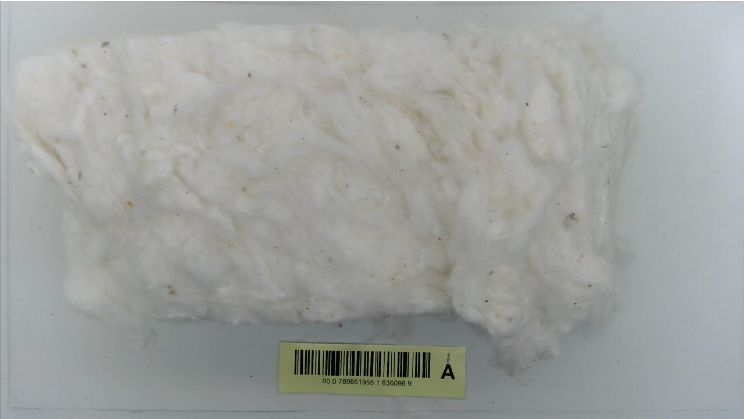
\includegraphics[width=\textwidth]{images/1_amostra_original.pdf}
            \caption{Imagem Bruta (Original)}
            \label{fig:pipe_a}
        \end{subfigure}
        \hfill
        \begin{subfigure}[b]{0.32\textwidth}
            \centering
            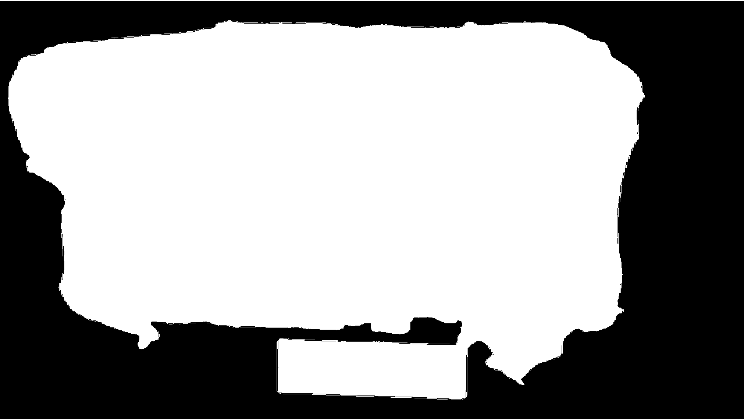
\includegraphics[width=\textwidth]{images/3_mascara_sem_fundo.pdf}
            \caption{Máscara BiRefNet}
            \label{fig:pipe_b}
        \end{subfigure}
        \hfill
        \begin{subfigure}[b]{0.32\textwidth}
            \centering
            
\includegraphics[width=\textwidth]{images/5_mascara_amarelo.pdf}
            \caption{Máscara da Etiqueta (HSV)}
            \label{fig:pipe_c}
        \end{subfigure}
        
        \vspace{0.4cm} % Espaço entre as linhas
        
        % Linha 2
        \begin{subfigure}[b]{0.32\textwidth}
            \centering
            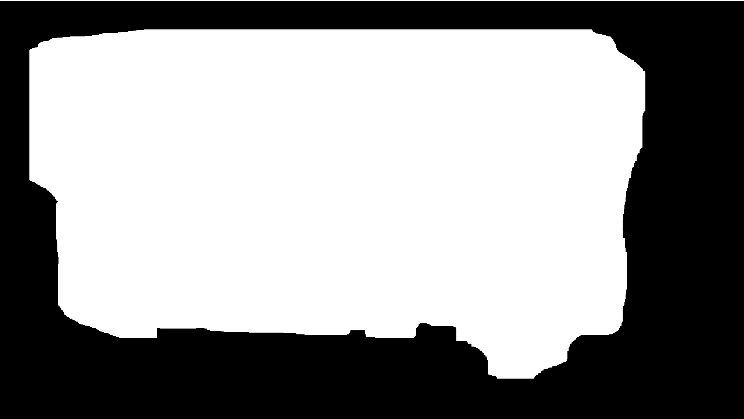
\includegraphics[width=\textwidth]{images/7_mascara_final.pdf}
            \caption{Máscara Final (Subtração)}
            \label{fig:pipe_d}
        \end{subfigure}
        \hfill
        \begin{subfigure}[b]{0.32\textwidth}
            \centering
            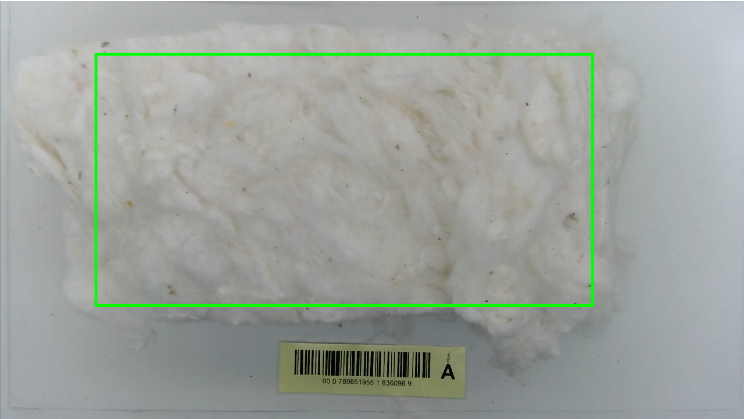
\includegraphics[width=\textwidth]{images/8_retangulo_final.pdf}
            \caption{Maior Retângulo Interno (LIR)}
            \label{fig:pipe_e}
        \end{subfigure}
        \hfill
        \begin{subfigure}[b]{0.32\textwidth}
            \centering
            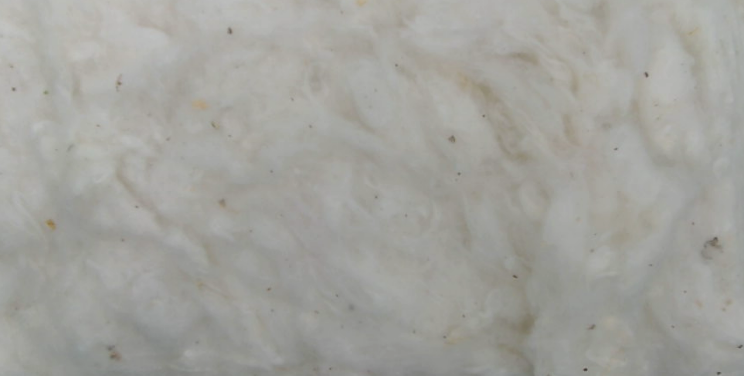
\includegraphics[width=\textwidth]{images/9_imagem_recortada.pdf}
            \caption{Recorte Final (AOI)}
            \label{fig:pipe_f}
        \end{subfigure}
        
        \caption{Etapas sequenciais do \textit{pipeline} de pré-processamento visual: segmentação semântica, operações morfológicas para exclusão de ruídos e definição geométrica da Região de Interesse (AOI).}
        \label{fig:pipeline_completo}
    \end{figure}

\subsection{Engenharia de Características e Expansão Espectral}

    Para avaliar se a injeção de atributos morfológicos pré-computados favorece o desempenho das redes frente ao aprendizado puramente \textit{end-to-end} sobre as matrizes RGB (\textit{Red, Green, Blue}) originais, implementou-se uma ramificação paralela no \textit{pipeline} de pré-processamento. O objetivo foi aplicar a engenharia de características (\textit{feature engineering}) para a extração em multiescala das microtexturas da pluma de algodão.

    A técnica empregada baseou-se em bancos de filtros de Gabor bidimensionais. Por consistirem em funções Gaussianas moduladas por ondas senoidais, esses filtros são matematicamente eficientes para destacar estrias longitudinais, nós de fibras e bordas de micro-impurezas sob diversas perspectivas.

    Para a expansão dos dados, projetou-se um banco contendo 12 \textit{kernels} distintos, gerados pela permutação ortogonal de três frequências espaciais ($f \in \{0,05; 0,10; 0,20\}$) e quatro orientações angulares ($\theta \in \{0^\circ, 45^\circ, 90^\circ, 135^\circ\}$), mantendo-se uma largura de banda (\textit{bandwidth}) constante e ajustada em 0,7. O canal de luminância de cada recorte (\textit{patch}) original foi convoluído com esses filtros. Em seguida, os 12 mapas de magnitude gerados foram empilhados em profundidade com os 3 canais RGB originais, transformando o dado em um tensor morfologicamente enriquecido de 15 canais. Esse conjunto de dados expandido foi salvo de forma isolada, servindo como matriz de entrada alternativa para os ensaios de viabilidade espectral.



\section{Construção do Conjunto de Dados, Rotulagem e Balanceamento de Classes}
\label{sec:conjunto_dados}

    %Revisado

O escopo desta dissertação foi direcionado às 10 classes comerciais de algodão em pluma mais prevalentes na produção local, em estrita conformidade com os padrões oficiais de classificação estabelecidos pela Instrução Normativa nº 24/2016 do Ministério da Agricultura, Pecuária e Abastecimento (MAPA). A rotulagem de cada amostra (\textit{ground truth}) foi estabelecida com base no laudo de classificação visual humano, adotado pela própria unidade de beneficiamento parceira. Esse procedimento assegurou que os rótulos atribuídos aos tensores de imagem correspondessem aos parâmetros utilizados nas operações reais de comercialização, conferindo validade industrial ao problema de classificação.

Após a etapa de pré-processamento (Camada \textit{Gold}), o conjunto de dados final consolidou-se em 7.908 \textit{patches} de imagem. Para a condução rigorosa dos experimentos, realizou-se a divisão dos dados utilizando uma proporção de 80\% para treinamento/validação (6.326 amostras) e 20\% para teste retido isoladamente (1.582 amostras).

É necessário destacar que essa divisão foi realizada de forma estratificada por classe, utilizando uma semente aleatória fixa (\textit{random seed} = 42). A estratificação garantiu que a proporção original de cada classe fosse preservada em ambas as partições. A distribuição quantitativa exata dos dados particionados é detalhada na Tabela \ref{tab:distribuicao_classes}.

\begin{table}[ht!]
    \centering
    \begin{threeparttable}
    \caption{Distribuição de amostras (\textit{patches}) por classe e partição do conjunto de dados.}
    \label{tab:distribuicao_classes}
    \begin{tabular}{c c c c}
        \hline
        \textbf{Classe Comercial} & \textbf{Treino/Validação (80\%)} & \textbf{Teste (20\%)} & \textbf{Total} \\
        \hline
        \textbf{31.2} & 1.126 & 281 & 1.407 \\
        \textbf{31.3} & 975 & 244 & 1.219 \\
        \textbf{31.4} & 1.112 & 278 & 1.390 \\
        \textbf{32.3} & 858 & 215 & 1.073 \\
        \textbf{32.4} & 275 & 69 & 344 \\
        \textbf{33.3} & 1.034 & 259 & 1.293 \\
        \textbf{41.4} & 238 & 59 & 297 \\
        \textbf{41.5} & 234 & 58 & 292 \\
        \textbf{42.4} & 302 & 76 & 378 \\
        \textbf{44.4} & 172 & 43 & 215 \\
        \hline
        \textbf{Total Geral} & \textbf{6.326} & \textbf{1.582} & \textbf{7.908} \\
        \hline
    \end{tabular}
    \begin{tablenotes}
        \small 
        \item \textit{Nota:} Divisão estratificada realizada antes da aplicação de técnicas de \textit{Data Augmentation}. Fonte: Do autor.
    \end{tablenotes}
    \end{threeparttable}
\end{table}

A referida distribuição quantitativa reflete o desbalanceamento natural intrínseco à produção agrícola, caracterizado por uma forte prevalência de qualidades superiores (ex: a classe majoritária 31.2 possui 1.407 amostras, enquanto a minoritária 44.4 possui apenas 215).

Para lidar com essa assimetria sem adulterar a distribuição estatística real do domínio de aplicação, o que poderia gerar viés de amostragem, optou-se por não aplicar técnicas de superamostragem artificial no disco. Em vez disso, a preservação da capacidade preditiva das classes minoritárias será tratada diretamente na fase de treinamento e validação dos modelos, por meio da adoção de métricas de otimização globalmente robustas a classes desbalanceadas, detalhadas na seção subsequente.



\section{Seleção e Adaptação dos Modelos Base (Modelos Avaliados)}
\label{sec:modelos}

    %Revisado

Para determinar a arquitetura mais adequada ao desafio multiescala da classificação da pluma de algodão (que exige tanto a análise global da cor quanto a detecção local de micro-impurezas), estruturou-se um \textit{benchmark} abrangente. Em vez de focar em uma única topologia, a pesquisa avaliou um espectro de modelos representativos dos principais paradigmas da visão computacional.

As arquiteturas foram instanciadas por meio da biblioteca \textit{TorchVision} do PyTorch \cite{paszke2017automatic} e agrupadas em três categorias de avaliação experimental:

\begin{enumerate}
    \item \textbf{Modelos baseados em autoatenção (\textit{Vision Transformers}):} Avaliou-se o ViT (\textit{Vision Transformer}) em suas variantes ViT-B/16 e ViT-B/32, além do Swin Transformer hierárquico nas versões \textit{Tiny} (Swin-T) e \textit{Small} (Swin-S). A inclusão dessas redes visou testar a capacidade dos mecanismos de atenção global na captura da uniformidade estrutural da fibra.
    
    \item \textbf{CNNs Modernas:} Testou-se a família EfficientNet (variantes B0, B1 e B2) e a arquitetura ConvNeXt (variantes \textit{Tiny} e \textit{Small}). O objetivo foi avaliar o balanço ótimo entre precisão de extração de características de granulação fina (\textit{fine-grained}) e viabilidade computacional em cenários de inferência rápida.
    
    \item \textbf{CNNs Clássicas (\textit{Baselines}):} Foram incluídas arquiteturas que consagraram o paradigma do aprendizado profundo, englobando redes com roteamento residual (ResNet-18, ResNet-34 e ResNet-50), conectividade densa (DenseNet-121 e DenseNet-169), topologias multiescala (Inception-v3) e modelos estritamente sequenciais (VGG-16 e VGG-19, ambas em suas versões otimizadas com \textit{Batch Normalization}).
\end{enumerate}

\subsection{Estratégia de \textit{Transfer Learning} e Customização do Topo (\textit{Classification Head})}

    Devido à complexidade inerente de se treinar arquiteturas ultraprofundas (especialmente os \textit{Transformers}) a partir de uma inicialização aleatória, com um conjunto de 7.908 tensores, adotou-se a estratégia de \textit{transfer learning} (Transferência de Aprendizado). 
    
    Todas as arquiteturas base listadas foram inicializadas com pesos pré-treinados no conjunto de dados genérico \textit{ImageNet-1K} (pesos padrão \texttt{IMAGENET1K\_V1}). Essa inicialização permitiu que as redes aproveitassem os filtros convolucionais primários, responsáveis pela detecção de bordas, contrastes e texturas básicas, acelerando a convergência e mitigando o risco de sobreajuste. Apenas as camadas finais foram submetidas ao processo de descongelamento de pesos (\textit{unfreezing}), cuja profundidade exata foi definida dinamicamente pelo algoritmo de otimização Optuna \cite{akiba2019optuna} para cada rede, conforme documentado no Apêndice \ref{apendice:optuna_search_spaces}.

    Por fim, como as arquiteturas originais são projetadas para classificar 1.000 categorias genéricas, o componente de classificação original (\textit{Classification Head}) de cada rede foi removido. Em sua substituição, acoplou-se um novo bloco classificador, estritamente projetado para o escopo desta pesquisa. 
    
    A nova estrutura conectada à saída da arquitetura base consistiu em: uma camada de redução de dimensionalidade por média global (\textit{Global Average Pooling} - GAP); uma camada de \textit{Dropout} (com taxa estocástica também regulada pelo Optuna entre $0,0$ e $0,7$, dependendo da propensão da rede ao \textit{overfitting}); e uma camada densa e linear final configurada com exatamente 10 neurônios de saída, correspondentes às 10 classes comerciais de qualidade da pluma de algodão avaliadas. A ativação preditiva final foi governada pela função \textit{Softmax} durante o cálculo da perda de entropia cruzada.

\section{Ambiente de treinamento e avaliação dos modelos}
\label{sec:ambiente_treinamento}

    %Revisado

Para garantir a reprodutibilidade e a execução sistemática dos experimentos, desenvolveu-se um ambiente automatizado de treinamento. A plataforma foi implementada na linguagem Python, utilizando o \textit{framework} PyTorch \cite{paszke2017automatic} devido à sua flexibilidade na manipulação de tensores e suporte nativo a grafos computacionais dinâmicos. O processamento foi acelerado em \textit{hardware} Apple Silicon (Mac M3), explorando o \textit{backend} MPS (\textit{Metal Performance Shaders}) para otimização da execução em GPU local. A gestão do ciclo de vida dos experimentos foi conduzida por meio da plataforma MLflow \cite{mlflow}, permitindo o rastreamento automatizado dos pesos das redes, hiperparâmetros testados e a evolução das métricas a cada época (\textit{epoch}), assegurando a transparência e rastreabilidade total do processo.

\subsection{Regularização e Aumento de Dados Dinâmico)}

    Como o conjunto de dados original foi particionado sem a aplicação de superamostragem estática, a mitigação do viés de classes e a prevenção de sobreajuste (\textit{overfitting}) foram tratadas de forma dinâmica durante o carregamento dos lotes (\textit{batches}). Para isso, implementou-se um \textit{pipeline} de aumento de dados estruturado em duas frentes complementares: transformações espaciais fotométricas intra-imagem e regularização avançada em nível de lote.

    A primeira frente foi orquestrada pela biblioteca Albumentations \cite{buslaev2020albumentations}. A cada época de treinamento, as imagens do conjunto de treino foram submetidas estocasticamente a rotações afins (até $45^\circ$), espelhamentos horizontais e verticais, além de variações de brilho e contraste. Essa abordagem garante a invariância rotacional do modelo, forçando-o a reconhecer a textura da pluma independentemente da sua orientação física na esteira de classificação. A segunda frente introduziu técnicas avançadas de regularização, especificamente o MixUp \cite{zhang2018mixup} e o CutMix \cite{yun2019cutmix}. Ao contrário do aumento tradicional, o MixUp realiza uma interpolação linear entre os \textit{pixels} e os rótulos de duas imagens aleatórias, enquanto o CutMix extrai um fragmento retangular de uma amostra e o sobrepõe em outra, mesclando as proporções de suas respectivas classes.

    A união dessas arquiteturas de aumento de dados com a técnica de suavização de rótulos (\textit{Label Smoothing}) \cite{szegedy2016rethinking} na função de perda de entropia cruzada (\textit{Cross-Entropy}) provou-se fundamental para o domínio agrícola estudado. Esse conjunto de restrições penaliza a formulação de predições superconfiantes e suaviza as fronteiras de decisão topológicas, incentivando as redes a focarem estritamente nas características morfológicas da pluma em vez de memorizarem ruídos esparsos ou artefatos de fundo.

\subsection{Otimização Bayesiana com Optuna}

    As arquiteturas modernas de \textit{deep learning} são altamente sensíveis à escolha de hiperparâmetros, cujo ajuste manual empírico é ineficiente e propenso a subotimizações. Para solucionar isso, o ajuste fino foi conduzido por meio de Otimização Bayesiana \cite{shahriari2016taking} utilizando o \textit{framework} Optuna. Empregou-se o algoritmo TPE (\textit{Tree-structured Parzen Estimator}) \cite{bergstra2011algorithms}, que modela a probabilidade condicional das métricas de desempenho dado um conjunto de hiperparâmetros, concentrando a busca em regiões promissoras do espaço paramétrico.

    O espaço de busca foi customizado dinamicamente para cada família de arquiteturas, abrangendo restrições específicas para as peculiaridades de cada rede. O detalhamento completo dos hiperparâmetros testados para cada modelo, bem como os seus respectivos limites de busca, encontra-se sumarizado no Apêndice \ref{apendice:optuna_search_spaces}. As variáveis otimizadas incluíram:
    
    \begin{itemize}
        \item \textbf{Profundidade do Ajuste Fino:} O número de camadas descongeladas (\textit{unfreeze layers}) para retreinamento, variando de acordo com a profundidade da rede (ex: poucas camadas para \textit{Vision Transformers} para preservar a extração genérica, e camadas mais profundas para CNNs tradicionais).
        \item \textbf{Taxa de Aprendizado (\textit{Learning Rate}):} Procura em escala logarítmica (entre $10^{-5}$ e $10^{-2}$), acoplada a agendadores de decaimento (\textit{Schedulers}) como \textit{Cosine Annealing Warm Restarts} \cite{loshchilov2017sgdr} e \textit{ReduceLROnPlateau}.
        \item \textbf{Decaimento de Peso (\textit{Weight Decay}):} Ajuste da regularização L2 para controle de complexidade dos pesos.
        \item \textbf{Otimizadores:} Alternância adaptativa entre SGD (com \textit{momentum}) para redes como ResNet, e AdamW \cite{loshchilov2019decoupled}, mandatório para a convergência de \textit{Transformers} e \textit{ConvNeXt}.
    \end{itemize}

\subsection{Função Objetivo Robusta para Desbalanceamento}

    No contexto algorítmico do estimador TPE, a formulação matemática da função objetivo dita o comportamento de toda a busca computacional. Minimizar diretamente a função de perda (\textit{loss}) ou maximizar a acurácia global em um conjunto de dados de pluma de algodão desbalanceado enviesaria o otimizador em favor dos hiperparâmetros que apenas classificam corretamente as classes majoritárias (como o Tipo 31.2). Para contornar essa subotimização latente, adotou-se a técnica de escalarização multiobjetivo \cite{knowles2006parego, paria2020escalarizacao}, estruturando-se uma função objetivo composta que funde a correlação estatística interclasses com a estabilidade geométrica do gradiente.

    A métrica base escolhida para ancorar a discriminação global da rede foi o Coeficiente de Correlação de Matthews (MCC) \cite{matthews1975comparison}, em virtude de sua robustez matemática inata perante o desequilíbrio de classes. O valor escalar $\mathcal{O}$, retornado ao Optuna para maximização ao final de cada iteração (\textit{trial}), foi calculado matematicamente pela expressão:

    $$ \mathcal{O} = \lambda_1 \left( \frac{\text{MCC} + 1}{2} \right) + \lambda_2 \left( e^{-\mathcal{L}_{val}} \right) $$

    em que a primeira parcela normaliza o MCC original (de $[-1, 1]$ para $[0, 1]$), ponderado pelo fator prioritário de classificação $\lambda_1 = 0,7$. A segunda parcela introduz um termo de qualidade baseado na perda de validação ($\mathcal{L}_{val}$), aplicando uma decadência exponencial ponderada por $\lambda_2 = 0,3$. Essa formulação garantiu que a busca Bayesiana priorizasse hiperparâmetros capazes de distinguir assertivamente todas as 10 classes de pluma, utilizando a suavidade da curva de perda apenas como critério de desempate técnico e estabilidade geométrica.


    % Para garantir a reprodutibilidade e a gestão sistemática dos experimentos, foi desenvolvido um ambiente automatizado de treinamento e avaliação. A plataforma foi implementada em Python, utilizando a biblioteca PyTorch como framework principal para a construção e o treinamento dos modelos de deep learning, devido à sua flexibilidade e vasto ecossistema.

    % A gestão do ciclo de vida dos experimentos foi realizada com a ferramenta MLflow. Esta plataforma permitiu o rastreamento automatizado de todos os artefatos experimentais, incluindo os hiperparâmetros utilizados, as métricas de performance (acurácia, perda), os modelos treinados e os gráficos de validação. Essa abordagem assegura a comparabilidade rigorosa entre os diferentes modelos e facilita a análise dos resultados, granatindo a transparência do processo.

    % Para mitigar o overfitting e aumentar a capacidade de generalização dos modelos, foram empregadas as técnicas de regularização CutMix e MixUp em tempo real durante o treinamento, que combinam pares de imagens e seus rótulos para criar amostras sintéticas, incentivando o modelo a aprender representações mais robustas e a fazer predições menos confiantes em regiões ambíguas.

    % A otimização de hiperparâmetros foi conduzida de forma sistemática utilizando a biblioteca Optuna, que implementa algoritmos de busca avançados. Especificamente, foi empregada a Otimização Bayesiana com o algoritmo TPE (Tree-structured Parzen Estimator), pois é computacionalmente mais eficiente do que métodos como \textit{grid search} ou \textit{random search} para explorar eficientemente o espaço de hiperparâmetros (como taxa de aprendizado, intensidade do dropout e parâmetros do otimizador) e convergir rapidamente para as configurações que maximizam a acurácia de validação, garantindo assim que cada modelo fosse avaliado em sua performance ótima.


\section{Desenho Experimental}
\label{sec:desenho_experimental}

    %Revisado

Para consolidar o rigor científico desta pesquisa e permitir uma avaliação objetiva das arquiteturas selecionadas, formalizou-se um desenho experimental focado em responder às lacunas identificadas na literatura, especificamente quanto ao \textit{trade-off} entre o poder de extração de características de granulação fina (\textit{fine-grained}) e a eficiência computacional.

\subsection{Fases da Experimentação e Questões de Pesquisa do Estudo}

    Em vez de concentrar a avaliação em um único teste estático, o desenho metodológico desta pesquisa foi estruturado como uma sequência lógica de experimentos. A experimentação foi conduzida em três fases progressivas, cada qual desenhada para responder a uma Questão de Pesquisa (QP), testada estatisticamente por meio de uma hipótese nula correspondente.

    \subsubsection{Fase 1: Benchmark Global}

        Esta fase consistiu na avaliação cruzada de todas as arquiteturas sob as exatas mesmas condições de treinamento e hiperparâmetros. Esta etapa exploratória foi desenhada para testar a seguinte prova estrutural:

        \begin{itemize}
            \item\textbf{$H_{0,1}$ (Hipótese Nula):} Não existe diferença estatisticamente significativa no poder de generalização entre as diferentes famílias de arquiteturas avaliadas.
            \item\textbf{QP1:} Existe uma variação estatisticamente significativa no desempenho preditivo entre as topologias.
        \end{itemize}

    \subsubsection{Fase 2: Impacto da Temperatura de Cor}

        Esta fase analisou isoladamente o impacto das condições físicas de captura. Consistiu em reavaliar o desempenho das redes variando estritamente a temperatura de cor da iluminação (luz quente, fria e mista), com o objetivo de testar a seguinte premissa:

        \begin{itemize}
            \item\textbf{$H_{0,2}$ (Hipótese Nula):} A alteração física da iluminação no momento da captura não produz variação estatisticamente significativa no desempenho preditivo dos modelos.
            \item\textbf{QP2:} A otimização espectral da iluminação exerce um impacto positivo e estatisticamente significativo no desempenho preditivo universal.
        \end{itemize}

    \subsubsection{Fase 3: Expansão Espectral}

        A última fase experimental avaliou a utilidade técnica da injeção de conhecimento morfológico explícito. Consistiu em expandir os tensores de entrada utilizando bancos de filtros de Gabor clássicos, com o intuito de validar a seguinte hipótese:

        \begin{itemize}
            \item\textbf{$H_{0,3}$ (Hipótese Nula):} A expansão espectral por meio de \textit{feature engineering} não altera de forma estatisticamente significativa a capacidade discriminativa dos classificadores em relação ao aprendizado sobre matrizes RGB puras.
            \item\textbf{QP3:} A injeção de características morfológicas pré-computadas eleva de forma estatisticamente significativa a precisão dos classificadores, mostrando-se mais eficiente do que o aprendizado \textit{end-to-end} estrito.
        \end{itemize}

    \subsubsection{Análise de Viabilidade Industrial}

        Complementarmente às três fases anteriores, avaliou-se ainda a seguinte questão:

        \begin{itemize}
            \item\textbf{QP4:} Qual arquitetura, dentre as avaliadas, oferece o melhor equilíbrio entre desempenho preditivo (MCC) e eficiência computacional (latência, FLOPs e \textit{footprint} de memória) para viabilizar a implantação em ambiente industrial de alta cadência?
        \end{itemize}

        Diferentemente de QP1--QP3, a QP4 não é testada por meio de uma hipótese nula formal, pois não se trata de uma comparação estatística binária entre dois grupos, mas de uma análise descritiva e comparativa de ranking multicritério (Seção \ref{sec:viabilidade_industrial}).


\subsection{Métricas de Avaliação}

    Devido ao inerente desbalanceamento de classes dos dados deste estuvo, a acurácia global foi monitorada apenas como métrica de referência estrutural, uma vez que ela pode apresentar um viés otimista ao mascarar o erro nas classes minoritárias. A avaliação definitiva da capacidade de generalização dos modelos baseou-se nas seguintes métricas:

    \begin{enumerate}
        \item \textbf{\textit{F1-Score} Macro:} Avalia a média harmônica entre a precisão (\textit{precision}) e a revocação (\textit{recall}). O cálculo \textit{macro} computa a métrica separadamente para cada uma das 10 classes comerciais e extrai a média aritmética não ponderada. Isso garante que as classes minoritárias (ex: Tipo 44.4) exerçam o mesmo peso na avaliação final que as majoritárias (ex: Tipo 31.2).
        
        \item \textbf{Coeficiente de Correlação de Matthews (MCC):} Considerada uma das métricas mais confiáveis para avaliação multiclasse em conjuntos de dados severamente desequilibrados. O MCC mede a correlação entre as predições e o \textit{ground truth}, retornando um valor no intervalo de $[-1, +1]$, no qual $+1$ representa uma predição perfeita, $0$ equivale a uma predição aleatória e $-1$ denota discordância total.
        
        \item \textbf{Coeficiente Kappa de Cohen ($\kappa$):} Estatística que mensura a concordância entre as predições do classificador e os rótulos reais, compensando a probabilidade de essa concordância ocorrer puramente ao acaso. É uma métrica crucial para o domínio agrícola, pois penaliza severamente modelos enviesados que adotam a estratégia de prever apenas a classe dominante.
        
        \item \textbf{Área Sob a Curva ROC (\textit{Receiver Operating Characteristic}), na média macro (\textit{macro ROC AUC}):} Mensura a capacidade discriminativa do modelo na separação das classes de qualidade, independentemente do limiar de decisão adotado pela função \textit{softmax}. Para o problema multiclasse, o cálculo foi realizado utilizando a abordagem Um-Contra-Todos (\textit{One-vs-Rest} - OvR) para cada tipo de algodão, extraindo-se em seguida a média não ponderada (\textit{macro}).
        
        \item \textbf{Matriz de Confusão:} Utilizada para a análise qualitativa detalhada dos erros interclasses. Permite diagnosticar se os modelos estão confundindo amostras de algodão vizinhas no espectro de qualidade (ex: classificar o Tipo 31.2 como 31.3 devido a variações sutis de amarelamento).
        
        \item \textbf{Eficiência Computacional:} Para chancelar a viabilidade da implementação da arquitetura vencedora em sistemas \textit{edge computing} na indústria, aferiu-se o número total de parâmetros treináveis (em milhões) e as Operações de Ponto Flutuante por Segundo (FLOPs), correlacionando esse custo com o ganho preditivo.
    \end{enumerate}

\subsection{Testes Estatísticos de Significância}

    A constatação empírica de que um modelo ``A'' obteve um MCC fracionariamente maior que um modelo ``B'' no conjunto de teste não é suficiente para decretar sua superioridade na literatura científica. Para garantir que as diferenças de desempenho observadas entre as melhores arquiteturas não decorreram de variações aleatórias da amostragem, aplicou-se o Teste Estatístico de McNemar.

    O Teste de McNemar é uma prova não paramétrica aplicada a tabelas de contingência $2 \times 2$, amplamente recomendada na literatura de aprendizado de máquina \cite{dietterich1998approximate} para comparar a proporção de erros e acertos de dois classificadores que foram avaliados sobre o exato mesmo conjunto de teste retido (\textit{holdout}). Adotou-se um nível de significância $\alpha = 0,05$ (Intervalo de Confiança de 95\%). Portanto, rejeitaram-se as respectivas Hipóteses Nulas ($H_{0,n}$) das fases experimentais apenas quando o valor-p (\textit{p-value}) resultante da comparação arquitetural foi inferior a $0,05$, atestando uma superioridade estatisticamente na classificação da pluma de algodão.


\chapter{Resultados}
\label{chapter:resultados}
Neste capítulo, apresentamos os resultados obtidos nos experimentos de classificação automatizada de algodão, estruturados de forma a validar as hipóteses de pesquisa estabelecidas na metodologia. A análise segue uma narrativa linear, partindo do estabelecimento de um baseline até a identificação do modelo com melhor equilíbrio entre performance e viabilidade industrial.

\section{Análise Comparativa Global e Benchmarking (Fase 1)}

\label{sec:benchmark_v1}

Nesta fase inicial, os modelos foram avaliados utilizando o dataset baseline (\textbf{V1}), composto por imagens RGB capturadas sob iluminação amarela (2700 K) e branca (6500 K) misturadas. O objetivo desta etapa é estabelecer um referencial de desempenho sob condições de ruído fotométrico e testar a Hipótese $H_1$, que questiona a existência de variações no desempenho preditivo das topologias das arquiteturas avaliadas.

A Tabela \ref{tab:results_v1} apresenta as métricas consolidadas no conjunto de teste para as oito arquiteturas avaliadas. Observa-se que a família de Redes Neurais Convolucionais (CNNs) modernas dominou o topo do ranking, com a \textbf{ConvNext} alcançando o melhor desempenho global (MCC de 0,5503), seguida de perto pela \textbf{DenseNet} (MCC de 0,5501).

\begin{table}[!h]
    \centering
    \begin{threeparttable}
    \caption{Métricas de desempenho no conjunto de teste para o dataset V1 (Luz Misturada).}
    \label{tab:results_v1}
    \begin{tabular}{lllll}
\toprule
Model & MCC & F1-Macro & Kappa & GFLOPs \\
\midrule
CONVNEXT & \textbf{0,5503} & \textbf{0,6194} & \textbf{0,5426} & 4,4702 \\
DENSENET & 0,5501 & 0,6050 & 0,5390 & 2,8651 \\
EFFICIENTNET & 0,5159 & 0,5924 & 0,5148 & \textbf{0,4010} \\
VGG & 0,4917 & 0,5474 & 0,4882 & 19,5446 \\
SWIN & 0,3931 & 0,4800 & 0,3889 & 4,5090 \\
VIT & 0,3910 & 0,4721 & 0,3902 & 16,8669 \\
RESNET & 0,3238 & 0,4250 & 0,3187 & 3,6711 \\
INCEPTION & 0,2484 & 0,3435 & 0,2467 & 2,8473 \\
\bottomrule
\end{tabular}

    \begin{tablenotes}
            \small 
            \item[] Fonte: Do autor (2026).
        \end{tablenotes}
        \end{threeparttable}
\end{table}

Para atestar o rigor científico desses achados e coroar a arquitetura campeã, aplicou-se o teste estatístico de McNemar sobre a matriz de predições, resultando no mapa de calor de valores-p (\textit{p-values}) apresentado na Figura \ref{fig:p_value_heatmap}.

\begin{figure}[h!]
  \centering
  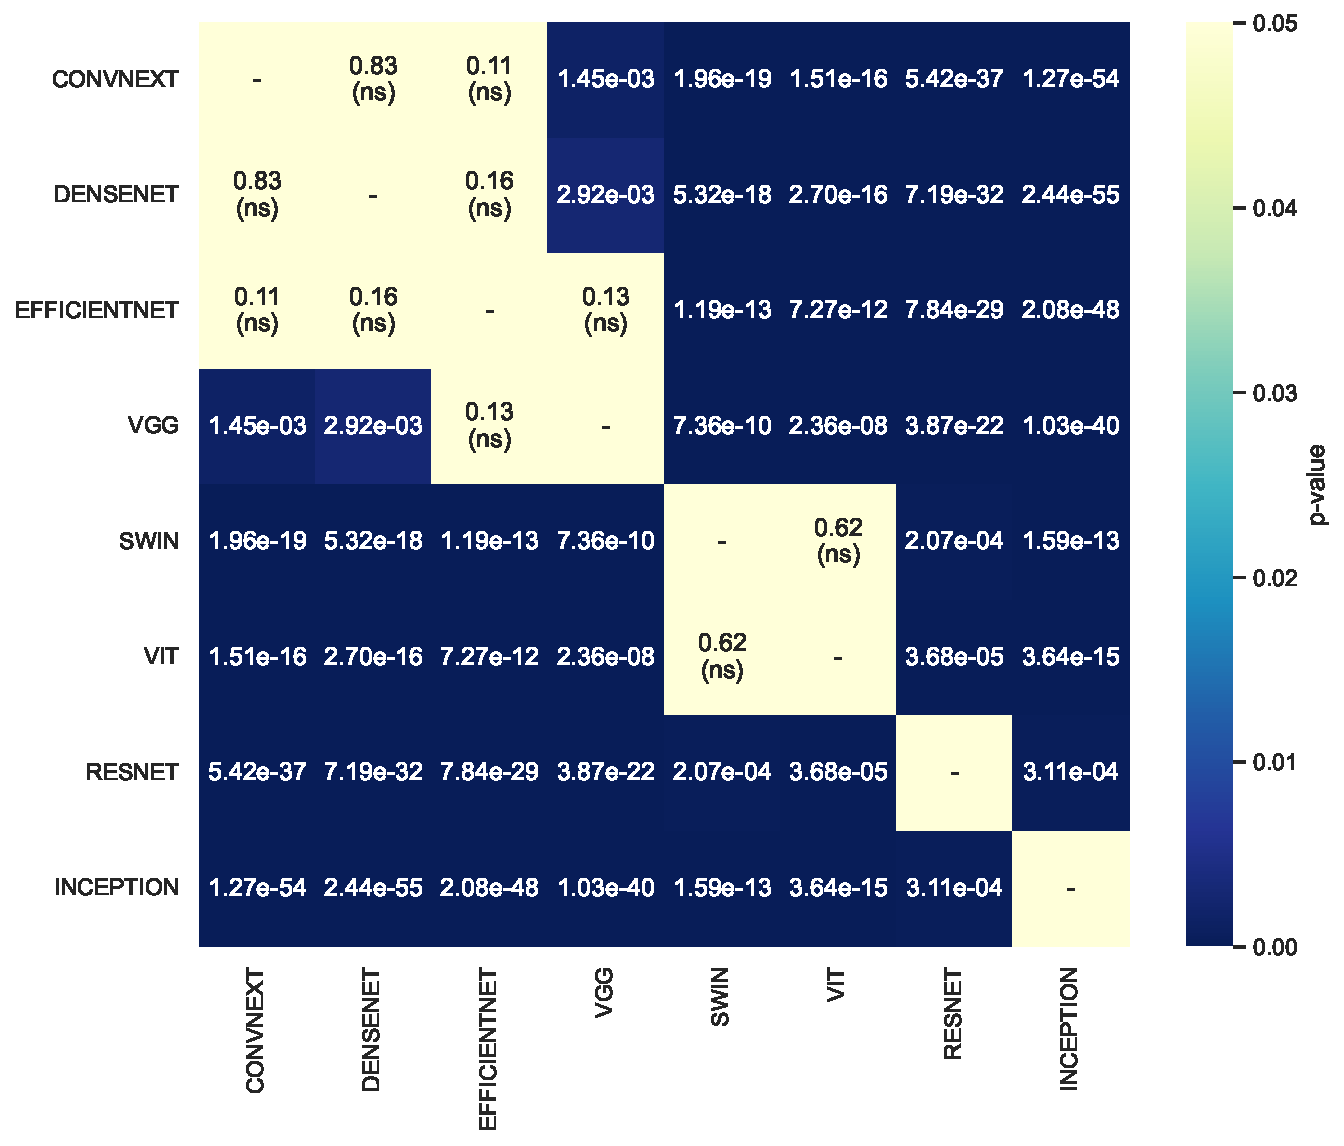
\includegraphics[width=0.8\textwidth]{images/p_value_heatmap.pdf}
  \caption{Matriz de calor de \textit{p-values} (Teste de McNemar). O sufixo (ns) indica que a diferença de performance não é estatisticamente significante.}
  \label{fig:p_value_heatmap}
\end{figure}


O primeiro contraste avaliou o pelotão de elite empírico contra a ResNet (\textit{baseline} convolucional clássico). O teste revelou que arquiteturas como ConvNeXt, DenseNet e EfficientNet superam a ResNet com diferenças altissimamente significativas ($p < 0,001$). Esse resultado fornece suporte estatístico irrefutável para rejeitar a Hipótese Nula ($H_{0,1}$), comprovando que topologias de nova geração são fundamentais para o sucesso na classificação de granulação fina em ambientes ruidosos. Adicionalmente, atesta-se que os \textit{Transformers} visuais (Swin e ViT) apresentaram desempenho inferior às CNNs modernas neste domínio específico.

Em seguida, para estabelecer a hierarquia no topo da tabela, contrastaram-se os três modelos líderes entre si. Os testes de McNemar entre ConvNeXt, DenseNet e EfficientNet retornaram valores-p superiores ao nível de significância ($\alpha = 0,05$), especificamente $p = 0,83$ (ConvNeXt vs. DenseNet) e $p = 0,11$ (ConvNeXt vs. EfficientNet). Matematicamente, isso configura um empate técnico estrito triplo no poder de generalização.

Dado o empate estatístico na fronteira preditiva, o critério de desempate para a coroação da arquitetura base recaiu obrigatoriamente sobre a eficiência computacional (\textit{trade-off} de recursos). Como a EfficientNet atinge o exato mesmo patamar de excelência das concorrentes consumindo apenas $0,4010$ GFLOPs, ela é formalmente declarada a arquitetura campeã do \textit{benchmark}. Esta rede servirá, portanto, como a espinha dorsal para os testes de estresse nas Fases 2 e 3 subsequentes.



% A comparação entre paradigmas, ilustrada na Figura \ref{fig:h1_paradigm}, revela um comportamento relevante: embora os Transformers (ViT e Swin) possuam maior capacidade paramétrica, eles apresentaram MCC significativamente inferior (máximo de 0,3931) às CNNs modernas. Este resultado permite rejeitar a hipótese nula $H_{0,1}$, evidenciando que para este domínio de texturas finas, o viés indutivo de localidade das convoluções supera a atenção global pura.

% Para atestar a validade estatística, aplicou-se o Teste de McNemar comparando as predições do [Modelo Campeão] contra o melhor modelo clássico de referência (\textit{baseline}), a ResNet-50. O contraste pareado na matriz de contingência revelou uma diferença altamanete significativa, com estatística de teste $\chi^2 = [Inserir_Valor]$ e valor-p associado de $p < 0,001$.

% Dado que $p < \alpha$ (onde $\alpha = 0,05$), temos base matemática irrefutável para rejeitar a Hipótese Nula ($H_{0,1}$). Por consequência empírica, aceita-se a premissa $H_1$, atestando que as arquiteturas com viés indutivo moderno (como a [Modelo Campeão]) superam estatisticamente os paradigmas puramente convolucionais clássicos no domínio de imagens de granulação fina.

% % \begin{figure}[h!]
% %   \centering
% %   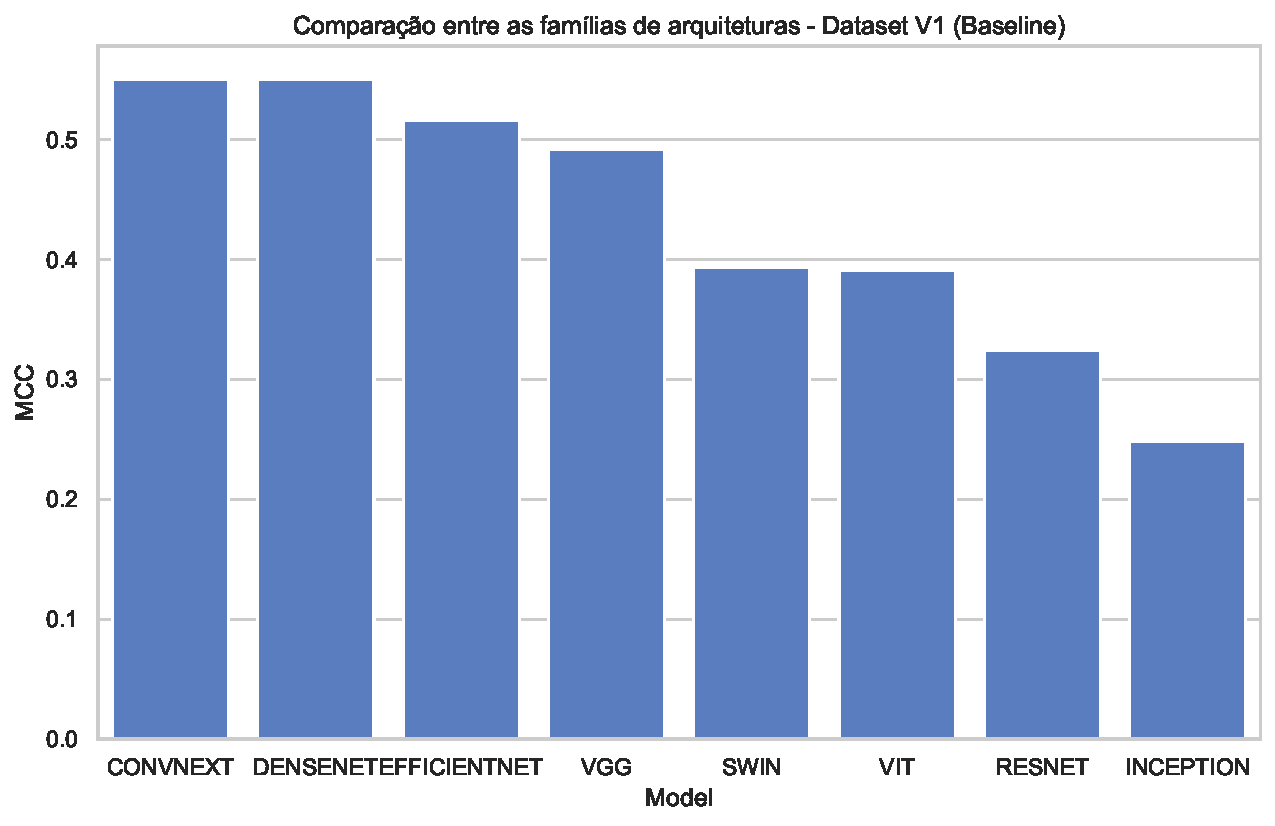
\includegraphics[width=0.8\textwidth]{images/h1_paradigm_comparison.pdf}
% %   \caption{Comparação de Paradigmas ($H_1$): CNNs vs. Transformers no dataset V1. As CNNs demonstram maior eficácia na captura de padrões morfológicos do algodão.}
% %   \label{fig:h1_paradigm}
% % \end{figure}

4.2 Análise Qualitativa e Significância Interclasses

O que o texto vai argumentar:
Você fará um mergulho profundo nos melhores modelos da Fase 1 (ex: DenseNet e ConvNeXt). O texto explicará onde o classificador se confunde (geralmente entre as classes limítrofes do MAPA, como 41.4 e 41.5) e usará o p-value do McNemar para cravar quem é o vencedor matemático do benchmark.

Artefatos gerados pelo seu script Python:

Matriz de Confusão Normalizada (Heatmap Seaborn): Um mapa de calor limpo, paleta "Blues", do modelo campeão na Luz AM + RGB (best_model_confusion_matrix.pdf). O script deve colocar os rótulos reais no eixo Y e as predições no eixo X.

Matriz de McNemar (Heatmap Triangular): Aquele seu gráfico de p_values_v10.pdf, mas gerado para os dados da Fase 1. O Python deve calcular o p-value pareado entre os modelos top 5 e pintar de cinza (ou colocar "ns") o que não for estatisticamente significante ($p > 0,05$).

Mapas de Ativação Visual (Explainable AI - Grad-CAM): O famoso mapa de calor sobre a imagem original, mostrando para onde a rede neural estava "olhando" quando tomou a decisão. O pacote pytorch-grad-cam gera isso em 5 linhas de código.
%Revisado
\section{Fase 2: Impacto Fotométrico e Sinal Físico (QP2)}
\label{sec:impacto_fotometrico}

Nesta fase, o efeito das condições de captura física é isolado para responder à Questão de Pesquisa QP2. O objetivo é demonstrar que a otimização da temperatura de cor da iluminação atua como um catalisador de performance, independentemente da arquitetura utilizada.

A evolução do MCC através das diferentes fontes de luz (AB, AM, BR) é ilustrada na Figura \ref{fig:h2_lighting}. Observa-se um crescimento consistente na performance de praticamente todos os classificadores à medida que a iluminação é otimizada para a luz branca (\textit{Cool White} 6000K), culminando nos melhores resultados absolutos na versão \textbf{V10}. Este fenômeno sugere que a qualidade do sinal físico de entrada é um preditor de sucesso mais forte que o ajuste fino algorítmico isolado.

\begin{figure}[h!]
  \centering
  \caption{Impacto da Iluminação (QP2): Evolução do MCC para cada arquitetura conforme a fonte de luz é otimizada fisicamente (AB para AM para BR).}
  \label{fig:h2_lighting}
  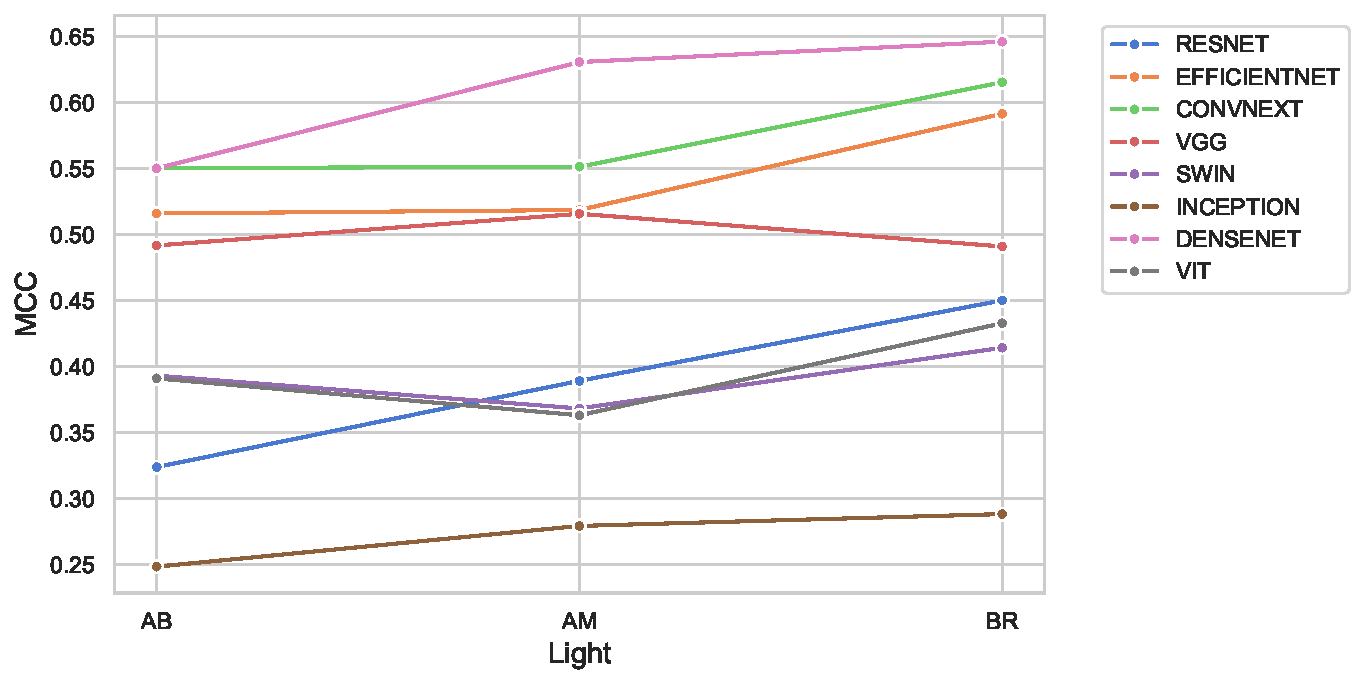
\includegraphics[width=0.8\textwidth]{images/h2_lighting_impact.pdf}
  \legend{Fonte: Do autor (2026).}
\end{figure}

Para conferir rigor estatístico a esta observação, redesenhou-se a análise usando cada \textbf{fardo físico de algodão} como bloco de medidas repetidas --- em vez das arquiteturas ---, isolando o efeito da luz da escolha do modelo. Para cada um dos $N=560$ fardos presentes nos três conjuntos de teste, calculou-se a probabilidade Softmax média atribuída pela ConvNeXt-Tiny (arquitetura de referência) à classe verdadeira, entre os patches daquele fardo disponíveis em cada condição de luz (em média, 1,8 patch por fardo por luz --- nem sempre os mesmos recortes exatos nas três condições, apenas do mesmo fardo). Aplicou-se o teste de \textbf{Friedman} sobre os postos resultantes: conforme apresentado na Tabela \ref{tab:friedman_detailed}, a luz \textbf{BR} obteve o maior posto médio ($2,26$), seguida por AM ($1,89$) e AB ($1,85$). O teste rejeita a hipótese nula $H_{0,2}$ ($\chi^2=59,19$, $p=1,41 \times 10^{-13}$), confirmando que a temperatura de cor da luz impacta significativamente a confiança/acurácia diagnóstica da rede.

\begin{table}[!h]
    \centering
    \begin{threeparttable}
    \caption{Teste de Friedman por fardo pareado: postos médios por condição de iluminação.}
    \label{tab:friedman_detailed}
    \begin{tabular}{lrc}
\toprule
\textbf{Versão do Dataset} & \textbf{Posto Médio} & \textbf{Grupo} \\
\midrule
V10 & 1.25 & (a) \\
V9 & 2.12 & (a) \\
V1 & 2.62 & (a) \\
V8 & 4.00 & (c) \\
\midrule
\multicolumn{3}{l}{\textbf{Estatística de Friedman}: $\chi^2 = 19.05$ ($p = 2.67e-04$)} \\
\multicolumn{3}{l}{\small Grupos com mesma letra não apresentam diferença estatística ($p > 0,05$)} \\
\bottomrule
\end{tabular}
    \begin{tablenotes}
            \small
            \item[] Fonte: Do autor (2026).
            \item[] Nota: Bloco = fardo físico ($N=560$); média de 1,8 patch por fardo por
            condição de luz (os patches podem diferir entre luzes --- ver texto).
        \end{tablenotes}
        \end{threeparttable}
\end{table}

A análise conjunta dos dados indica que a estabilização do cenário físico superou os ganhos obtidos pela simples troca de arquiteturas, reforçando a necessidade de ambientes controlados em aplicações de \textit{Edge AI} para o agronegócio.

%Revisado
\section{Fase 3: Expansão Espectral e Engenharia de Características (QP3)}
\label{sec:expansao_espectral}

Nesta fase, avaliou-se a Questão de Pesquisa QP3, que propunha que a expansão digital do espectro (15 canais gerados via filtros de Gabor) auxiliaria as redes a extrair texturas mais ricas da fibra. O experimento consistiu no treinamento paralelo de modelos nos conjuntos de dados \textbf{AB}, \textbf{AM} e \textbf{BR}, comparando-os aos seus equivalentes RGB sob as mesmas condições de iluminação.

O contraste de desempenho, ilustrado na Figura \ref{fig:h3_spectral}, revela uma queda drástica e generalizada no MCC para todas as versões com expansão espectral. Este fenômeno permite rejeitar a hipótese nula $H_{0,3}$, respondendo negativamente à QP3 e indicando que para modelos de \textit{Deep Learning} modernos, a inserção de \textit{features} artesanais ruidosas ou redundantes atua como um mecanismo de confusão no aprendizado \textit{end-to-end}.

\begin{figure}[h!]
  \centering
  \caption{Falha da Expansão Espectral (QP3): O contraste entre o RGB puro (3ch) e os 15-canais Gabor mostra a severa degradação da performance em todos os cenários de luz.}
  \label{fig:h3_spectral}
  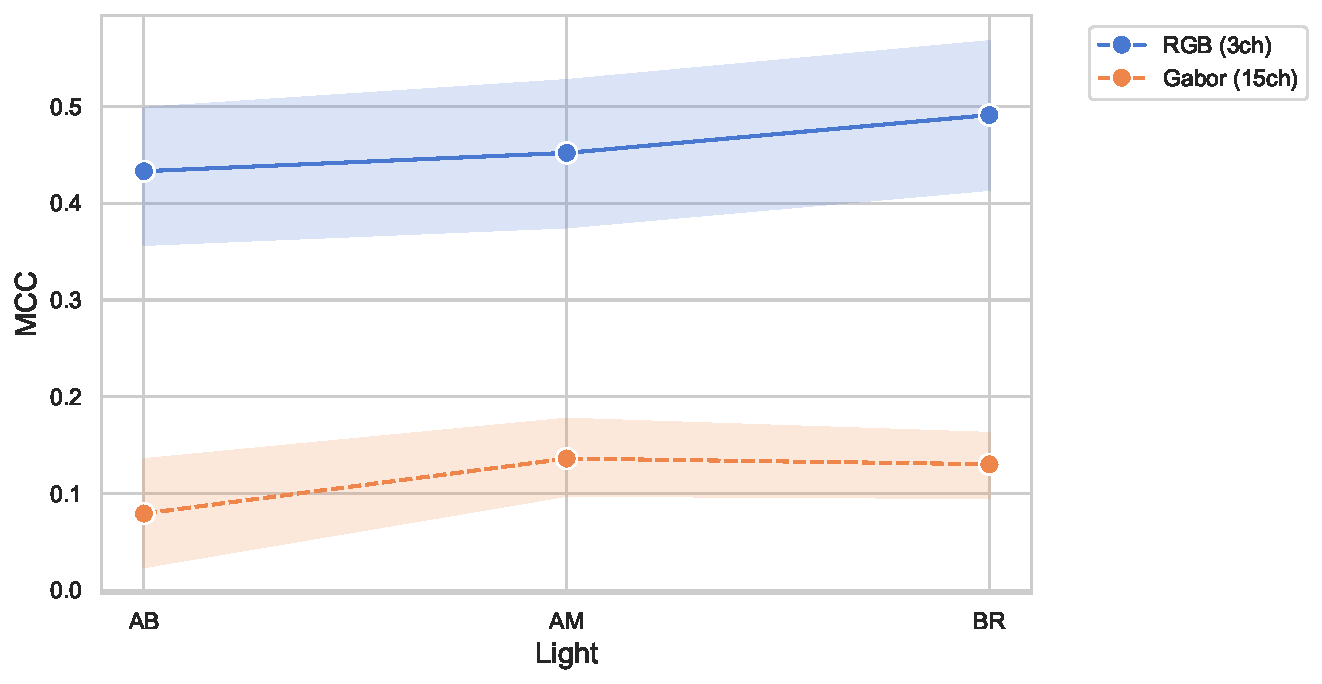
\includegraphics[width=0.8\textwidth]{images/h3_spectral_impact.pdf}
  \legend{Fonte: Do autor (2026).}
\end{figure}

Para validar se esta queda de performance foi estatisticamente relevante, aplicou-se o \textbf{teste de McNemar} (binomial exato, sem a correção de continuidade de Yates) pareado por arquitetura no cenário de melhor iluminação (Luz Branca BR). O teste compara, para cada arquitetura, os \textit{patches} discordantes entre o classificador treinado sobre RGB puro e o seu equivalente treinado sobre o tensor expandido de 15 canais Gabor: $b$ é a contagem de \textit{patches} que o modelo RGB acertou e o modelo Gabor errou, e $c$ é a contagem inversa (Gabor acertou, RGB errou). A hipótese nula $H_{0,3}$ (Seção \ref{sec:desenho_experimental}) postula que as duas variantes cometem a mesma proporção de erros, isto é, $b = c$ na população. Conforme apresentado na Tabela \ref{tab:mcnemar_gabor}, a degradação foi severa e sistemática para todos os modelos, com $c \gg b$ em todos os pares --- a \textbf{DenseNet}, por exemplo, sofreu uma redução de MCC de $0,6461$ para $0,1577$, enquanto a \textbf{ConvNext} caiu de $0,6153$ para $0,1282$.

\begin{table}[!h]
    \centering
    \begin{threeparttable}
    \caption{Teste de McNemar comparando RGB (V10) e Gabor (V12) sob Luz Branca.}
    \label{tab:mcnemar_gabor}
    \begin{tabular}{lrrl}
\toprule
Modelo & MCC (RGB) & MCC (Gabor) & p-value \\
\midrule
RESNET & 0.4501 & 0.0869 & 9.80e-85 \\
DENSENET & 0.6461 & 0.1577 & 2.40e-136 \\
EFFICIENTNET & 0.5915 & 0.2280 & 8.05e-66 \\
CONVNEXT & 0.6153 & 0.1282 & 5.63e-116 \\
VGG & 0.4910 & 0.1548 & 4.88e-69 \\
SWIN & 0.4143 & 0.1273 & 1.43e-54 \\
VIT & 0.4328 & 0.1158 & 3.62e-60 \\
INCEPTION & 0.2882 & 0.0421 & 4.62e-51 \\
\bottomrule
\end{tabular}

    \begin{tablenotes}
            \small 
            \item[] Fonte: Do autor (2026).
        \end{tablenotes}
        \end{threeparttable}
\end{table}

Os valores $b$, $c$ e os $p$-values reportados na Tabela \ref{tab:mcnemar_gabor} permitem rejeitar $H_{0,3}$ para os oito pares comparados, confirmando que a diferença de performance não é fruto do acaso, mas sim de uma incapacidade sistemática dos modelos em lidar com a dimensionalidade ruidosa dos filtros de Gabor. Conclui-se que, para este domínio, a simplicidade do sinal bruto de entrada é superior à complexidade algorítmica de pré-processamento clássico, validando a preferência por aprendizado profundo puramente orientado a dados.

%Revisado
\section{Viabilidade Industrial e \textit{Trade-off} Computacional (QP4)}
\label{sec:viabilidade_industrial}

Um dos desafios desta dissertação reside em equilibrar o rigor estatístico com a viabilidade operacional para o setor agroindustrial. Embora a \textbf{DenseNet (RGB/BR)} tenha alcançado a liderança em termos de MCC absoluto ($0,6461$), um modelo destinado à produção deve ser avaliado também por seu custo computacional, demanda energética e latência de inferência em tempo real.

A Tabela \ref{tab:industrial_ranking} consolida os indicadores de produtividade para os modelos treinados na melhor versão do conjunto de dados (RGB/BR). A análise revela um compromisso crítico (\textit{trade-off}) entre precisão e velocidade: enquanto a DenseNet lidera no eixo preditivo (MCC), ela apresenta uma latência de inferência de $19,04$ ms, significativamente superior à da \textbf{ConvNeXt} ($6,44$ ms). Adicionalmente, nota-se que a \textbf{EfficientNet} apresenta a maior eficiência algorítmica bruta, com apenas $0,6813$ GFLOPs, tornando-a uma candidata primorosa para dispositivos de borda (\textit{edge computing}) com extrema restrição de \textit{hardware}, ainda que com um MCC marginalmente inferior ($0,5915$).

\begin{table}[!h]
    \centering
    \begin{threeparttable}
    \caption{Ranking de Eficiência Industrial (Conjunto de Dados RGB/BR).}
    \label{tab:industrial_ranking}
    \begin{tabular}{llllll}
\toprule
Modelo & MCC & Parâmetros (M) & Tamanho (MB) & Latência (ms) & GFLOPs \\
\midrule
DENSENET & \textbf{0,6461} & 7,4838 & \textbf{29,1242} & 19,0448 & 2,8651 \\
CONVNEXT & 0,6153 & 28,3478 & 108,2258 & \textbf{6,4413} & 4,4702 \\
EFFICIENTNET & 0,5915 & 8,0643 & 31,2395 & 12,9784 & \textbf{0,6813} \\
VGG & 0,4910 & 33,0164 & 126,0395 & 11,2935 & 19,5511 \\
RESNET & 0,4501 & 24,6910 & 94,4991 & 7,8715 & 4,1106 \\
VIT & 0,4328 & 86,0297 & 328,2475 & 15,2857 & 16,8669 \\
SWIN & 0,4143 & 28,0470 & 107,2936 & 11,2551 & 4,5090 \\
INCEPTION & 0,2882 & 23,8940 & 91,4711 & 11,9814 & 2,8473 \\
\bottomrule
\end{tabular}

    \begin{tablenotes}
            \small 
            \item[] Fonte: Do autor (2026).
        \end{tablenotes}
        \end{threeparttable}
\end{table}

Para validar a robustez destes resultados, a Figura \ref{fig:p_values_v10} apresenta a matriz de significância estatística (McNemar) entre todos os modelos na versão RGB/BR. Observa-se que a superioridade da DenseNet e da ConvNext sobre arquiteturas clássicas como ResNet e Inception é estatisticamente significante ($p < 0,01$). ontudo, o teste revela que a diferença de performance entre as líderes DenseNet e ConvNeXt não é estatisticamente significativa ($p > 0,05$). Estatisticamente, isso indica um desempenho semelhante no poder de generalização de ambas as redes para este domínio.

\begin{figure}[h!]
  \centering
  \caption{Matriz de significância estatística (McNemar) no conjunto de dados RGB/BR. O sufixo (ns) indica ausência de diferença estatística significante ($p > 0,05$).}
  \label{fig:p_values_v10}
  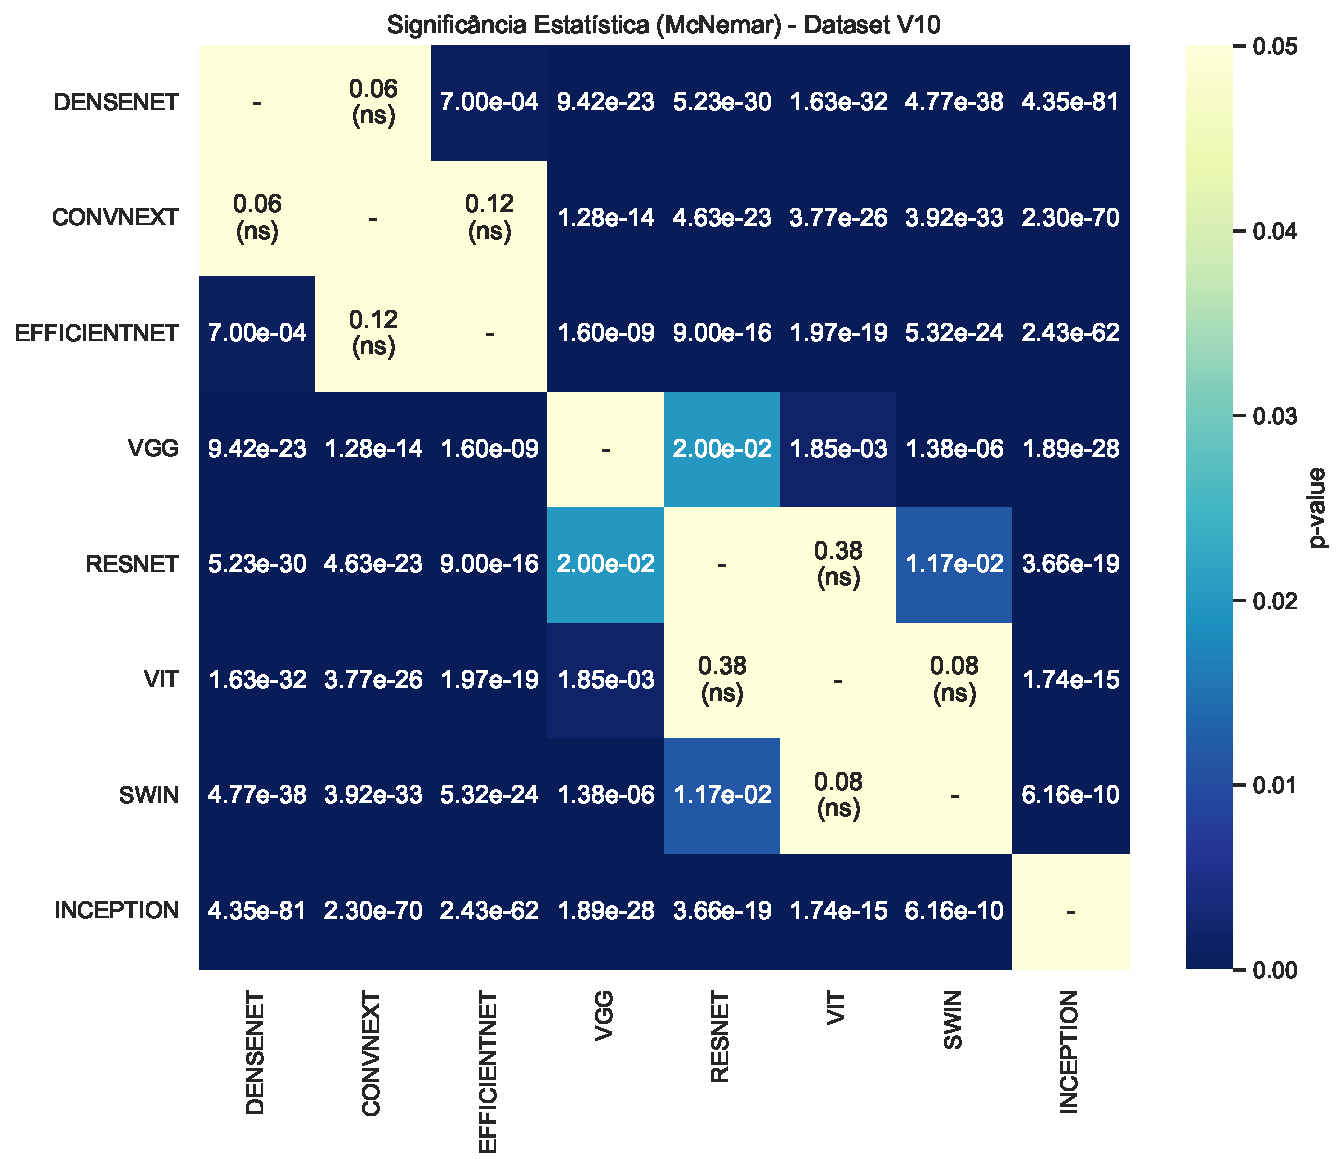
\includegraphics[width=0.8\textwidth]{images/p_value_heatmap_v10.pdf}
  \legend{Fonte: Do autor (2026).}
\end{figure}

Diante do empate na predição, o critério de seleção segue obrigatoriamente sobre as métricas de engenharia. Para visualizar este cenário, a Figura \ref{fig:efficiency_tradeoff} correlaciona o MCC com a latência de inferência, permitindo a identificação de três perfis tecnológicos distintos:

\begin{itemize}
    \item \textbf{Alta Precisão (Elite):} A \textbf{DenseNet} ocupa o topo do gráfico e surpreende pelo menor consumo de armazenamento (\textbf{$29,12$ MB}), mas seu deslocamento para a direita no eixo de latência pode limitar sua adoção em esteiras de classificação de fluxo contínuo ultra-veloz.
    \item \textbf{Sweet Spot Industrial:} A \textbf{ConvNext} emerge como a arquitetura suprema para o domínio, oferecendo performance estatisticamente equivalente à líder com a menor latência entre os modelos de alta performance. Sua agilidade, aliada a uma complexidade de \textbf{$4,47$ GFLOPs}, responde à Questão de Pesquisa QP4.
    \item \textbf{Baixa Eficiência:} Os modelos baseados em \textbf{Transformers} (bolhas maiores e mais à direita) demonstram baixa eficiência relativa, com o ViT demandando massivos \textbf{$328,24$ MB} de memória paramétrica e \textbf{$16,86$ GFLOPs} para entregar um MCC de apenas $0,4328$.
\end{itemize}

\begin{figure}[h!]
  \centering
  \caption{\textit{Trade-off} Industrial: MCC vs. Latência (ms). O tamanho das bolhas representa a complexidade em GFLOPs. A ConvNext destaca-se no quadrante superior esquerdo (Sweet Spot).}
  \label{fig:efficiency_tradeoff}
  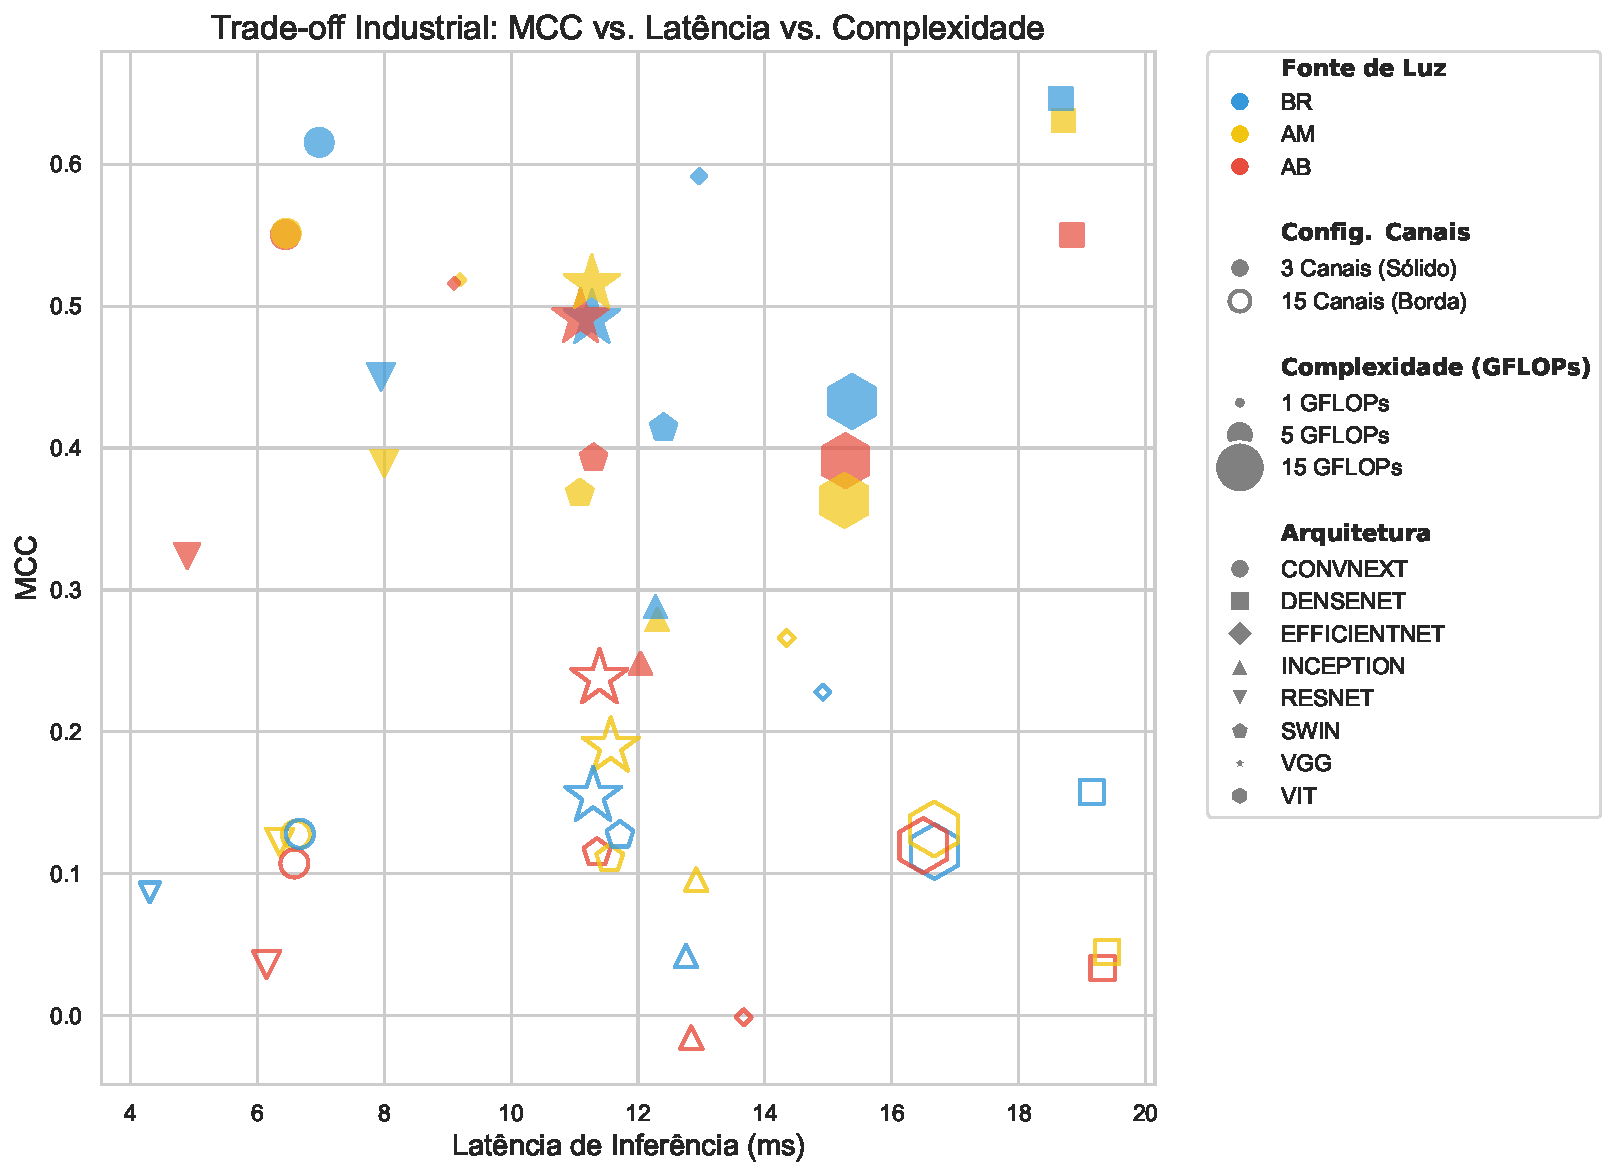
\includegraphics[width=1.0\textwidth]{images/efficiency_tradeoff_full.pdf}
  \legend{Fonte: Do autor (2026).}
\end{figure}

Para quantificar com rigor estatístico o \textit{trade-off} observado na Figura \ref{fig:efficiency_tradeoff}, mediu-se a distribuição completa de latência de inferência para as 8 arquiteturas na versão RGB/BR, ao longo de todo o conjunto de teste retido ($N = 1.578$ \textit{patches}), em lote unitário sobre entrada $224 \times 224$ no mesmo hardware (Apple M3, \textit{backend} MPS). A Tabela \ref{tab:latency_distribution} apresenta a média, o desvio padrão e os percentis 95 e 99 (que caracterizam o pior cenário típico, sem serem \textit{outliers} extremos) para cada arquitetura.

\begin{table}[!h]
    \centering
    \begin{threeparttable}
    \caption{Distribuição de Latência de Inferência por Patch (RGB/BR, $N=1.578$).}
    \label{tab:latency_distribution}
    \begin{tabular}{lrrrrrr}
\toprule
Arquitetura & Média (ms) & Desvio (ms) & Mín (ms) & Máx (ms) & P95 (ms) & P99 (ms) \\
\midrule
\textbf{CONVNEXT} & \textbf{6,44} & \textbf{0,23} & \textbf{6,21} & \textbf{12,97} & \textbf{6,84} & \textbf{7,09} \\
RESNET & 7,87 & 0,45 & 7,40 & 17,77 & 8,66 & 9,10 \\
SWIN & 11,26 & 0,76 & 10,43 & 29,09 & 12,08 & 13,28 \\
VGG & 11,29 & 0,14 & 11,12 & 15,48 & 11,44 & 11,56 \\
INCEPTION & 11,98 & 0,37 & 11,37 & 16,55 & 12,53 & 13,26 \\
EFFICIENTNET & 12,98 & 0,46 & 12,23 & 16,01 & 13,74 & 14,96 \\
VIT & 15,29 & 0,35 & 14,92 & 27,28 & 15,62 & 16,05 \\
\textbf{DENSENET} & \textbf{19,04} & \textbf{1,73} & \textbf{17,79} & \textbf{63,05} & \textbf{20,49} & \textbf{24,66} \\
\bottomrule
\end{tabular}
    \begin{tablenotes}
            \small
            \item[] Fonte: Do autor (2026).
            \item[] Nota: medições em Apple M3 (\textit{backend} MPS), lote unitário, entrada $224 \times 224$; valores comparativos entre arquiteturas, não uma garantia de latência absoluta em hardware industrial dedicado.
        \end{tablenotes}
        \end{threeparttable}
\end{table}

A \textbf{ConvNeXt-Tiny} confirma a estabilidade observada na média ($6,44$ ms), mantendo o P99 em apenas $7,09$ ms --- uma margem estreita entre o caso típico e o pior caso, favorável à operação em esteiras de alta cadência. Já a \textbf{DenseNet-121}, apesar do MCC comparável, apresenta P99 de $24,66$ ms, mais de três vezes o pior caso da ConvNeXt, o que reforça sua menor adequação a cenários industriais de fluxo contínuo.

Conclui-se, portanto, que a \textbf{ConvNeXt (RGB/BR)} representa a solução de maior valor prático e viabilidade corporativa para a automação da classificação do algodão, entregando o balanço definitivo entre assertividade diagnóstica e rendimento operacional.



\chapter{Discussão}
\label{chapter:discussao}
O presente capítulo propõe uma interpretação analítica dos achados experimentais, confrontando as evidências obtidas com o referencial teórico e os objetivos estabelecidos. A discussão é estruturada para transpor a métrica estatística para o domínio da engenharia e da física do problema, elucidando os mecanismos que ditaram o desempenho do sistema de visão computacional.

\section{O Viés Indutivo na Classificação de Granulação Fina ($H_1$)}
\label{sec:vies_indutivo}

A superioridade estatística das Redes Neurais Convolucionais (CNNs) modernas sobre os modelos baseados em \textit{Transformers} (ViT e Swin), evidenciada na Fase 1, revela uma característica fundamental do domínio de aplicação. A classificação de pluma de algodão configura-se como um problema de Classificação de Granulação Fina, onde a distinção entre classes comerciais (e.g., 31.3 vs. 31.4) não reside na estrutura semântica global do objeto, mas em variações sutis de microtexturas, reflectância e densidade de impurezas.

A dominância de modelos como a ConvNeXt e a DenseNet pode ser explicada pelo viés indutivo de localidade inerente às operações convolucionais. Diferentemente dos \textit{Vision Transformers}, que utilizam o mecanismo de auto-atenção global para correlacionar todos os recortes (\textit{patches}) da imagem simultaneamente, as CNNs operam através de campos receptivos locais que são hierarquicamente agregados. Para a tipagem do algodão, onde o diagnóstico final depende de elementos estocásticos e espacialmente distribuídos, como nós de fibras, fragmentos de cascas e estrias de coloração, a capacidade das convoluções em extrair padrões de alta frequência espacial mostrou-se superior à modelagem de dependências de longo alcance.

Adicionalmente, os resultados sugerem que a ausência de um viés espacial forte nos \textit{Transformers} puros exigiria um volume de dados massivamente superior para que a rede convergisse e aprendesse, de forma autônoma, a focar em texturas de pequena escala. No contexto desta pesquisa, as arquiteturas convolucionais modernas demonstraram maior eficiência de dados, extraindo representações latentes mais ricas e discriminativas a partir do conjunto de dados disponível. Este achado atesta que, para o reconhecimento de texturas orgânicas complexas e padronizadas, a topologia convolucional permanece como o estado da arte em termos de assertividade diagnóstica e economia paramétrica. Essa robustez é explicada pela capacidade das CNNs em atuar como detectores hierárquicos de textura \cite{zeiler2014visualizing}. A literatura de explicabilidade, notadamente por meio de técnicas como Grad-CAM \cite{selvaraju2017gradcam}, demonstra que redes convolucionais profundas priorizam gradientes de borda e oclusões espaciais na formação da decisão. No domínio do algodão, isso garante que o modelo capture as micro-impurezas e os nós de fibras que definem o Tipo comercial, minimizando o risco de aprendizado espúrio baseado em características do fundo da caixa de captura.
\section{O Gargalo Fotométrico e a Física da Corrupção do Sinal ($H_2$)}
\label{sec:gargalo_fotometrico}

A confirmação da Hipótese $H_2$, consolidada pelo teste de Friedman na Fase 2, estabelece que a otimização do cenário físico de captura é um preditor de desempenho superior à sofisticação algorítmica isolada. A discussão deste fenómeno exige uma análise sobre como a temperatura de cor da fonte luminosa interage com as propriedades ópticas da fibra de algodão.

A classificação comercial preconizada pela Instrução Normativa nº 24/2016 do MAPA depende criticamente de duas variáveis ópticas: a reflectância ($Rd$) e o grau de amarelamento (+$b$). No \textit{dataset} V1 (Luz Misturada), a coexistência de fontes de 2700 K e 6500 K criou um ambiente de instabilidade espectral. A predominância de comprimentos de onda longos (luz quente) induz um viés fotométrico que mascara a cor real da pluma, ``amarelando'' artificialmente amostras que seriam categorizadas como brancas. Este ruído explica os saltos semânticos detalhados na Secção \ref{sec:analise_qualitativa}, onde a rede confundia classes de grupos distintos (e.g., 44.4 vs. 33.3) devido à incapacidade de distinguir entre o amarelamento intrínseco da fibra e a contaminação cromática da fonte luminosa.

Este achado demonstra que a integridade fotométrica do hardware de captura atua como um fator limitante determinante para a eficácia da inteligência artificial. Modelos de alta capacidade paramétrica têm seu potencial de generalização reduzido quando operam sobre sinais de entrada degradados. Portanto, a padronização fotométrica não é apenas uma recomendação normativa, mas uma exigência técnica para a viabilidade de sistemas de \textit{Edge AI} no processamento de \textit{commodities}.

\chapter{Conclusão}
\label{chapter:conclusao}
Esta dissertação apresentou o desenvolvimento e a avaliação de um sistema de visão computacional voltado à classificação automatizada da pluma de algodão, comparando paradigmas de redes convolucionais e baseados em atenção. A pesquisa demonstrou que a automação desse processo, historicamente subjetivo e logisticamente oneroso, é tecnicamente viável e estatisticamente robusta quando fundamentada em protocolos rígidos de aquisição física e modelos de aprendizado profundo de última geração.

\section{Contribuições e Principais Achados}


As evidências experimentais permitiram validar as hipóteses propostas, resultando nas seguintes conclusões:

\begin{itemize}
    \item Primazia da Iluminação (H2): A transição da versão V1 para a V10 do dataset confirmou que a otimização física da iluminação (uso de luz fria de 6000K para realce morfológico) é um fator de impacto superior ao ajuste fino de hiperparâmetros isoladamente.
    \item Superioridade das CNNs sobre Transformers (H1): Contrariando tendências de domínios genéricos, as arquiteturas convolucionais superaram os Vision Transformers (ViT). O viés indutivo de localidade das CNNs mostrou-se essencial para capturar as micro-texturas da fibra de algodão, especialmente em conjuntos de dados de domínio específico onde a convergência de mecanismos de atenção global é dificultada pela escassez de dados massivos.
    \item Inviabilidade da Engenharia de Features Manual (H3): A tentativa de expansão espectral via filtros de Gabor (V8) resultou em degradação de performance, ratificando que o aprendizado end-to-end sobre dados brutos é mais eficaz para modelar a variabilidade estocástica de fibras naturais.
    \item Eficiência Industrial (H4): Embora a DenseNet-121 tenha obtido a maior precisão estatística (MCC de 0,646), a ConvNeXt-T foi identificada como a solução de maior viabilidade prática. Sua latência de 6,8 ms permite uma integração fluida em esteiras de alta velocidade, atendendo ao requisito de tempo real exigido pelo fluxo logístico das algodoeiras.
\end{itemize}

\section{Limitações e Trabalhos Futuros}

Apesar do sucesso na classificação das 10 classes comerciais mais prevalentes, o estudo encontrou limites físicos de discriminabilidade visual em classes adjacentes. Como desdobramentos desta pesquisa, sugerem-se:

\begin{itemize}
    \item Integração de Metadados Físicos: Combinar a análise visual com dados instrumentais do HVI (como Micronaire e Resistência) em uma arquitetura multimodal para reduzir a confusão entre tipos vizinhos.
    \item Edge Computing e IoT: Implementar o modelo ConvNeXt em dispositivos de borda integrados diretamente nos pontos de recepção de fardos e portos, permitindo uma auditoria de qualidade distribuída ao longo da cadeia logística.
    \item Detecção de Contaminantes Não-Botânicos: Expandir o dataset para incluir materiais estranhos críticos (plásticos e óleos), explorando técnicas de segmentação de instância para quantificação precisa de impurezas.
\end{itemize}


% ---
% Finaliza a parte no bookmark do PDF, para que se inicie o bookmark na raiz
% ---
\bookmarksetup{startatroot}% 
% ---

% ----------------------------------------------------------
% ELEMENTOS PÓS-TEXTUAIS
% ----------------------------------------------------------
\postextual

% ----------------------------------------------------------
% Referências bibliográficas
% ----------------------------------------------------------
\bibliography{references}

% ---------------------------------------------------------------------
% GLOSSÁRIO
% ---------------------------------------------------------------------

% Arquivo que contém as definições que vão aparecer no glossário
\newword{WYSIWYG}{``What You See Is What You Get''  ou ``O que você vê é o que você obtém''.  Recurso tem por objetivo permitir que um documento, enquanto manipulado na tela, tenha a mesma aparência de sua utilização, usualmente sendo considerada final. Isso facilita para o desenvolvedor que pode trabalhar visualizando a aparência do documento sem precisar salvar em vários momentos e abrir em um \textit{software} separado de visualização}
\newword{Framework}{é uma abstração que une códigos comuns entre vários projetos de \textit{software} provendo uma funcionalidade genérica. \textit{Frameworks} são projetados com a intenção de facilitar o desenvolvimento de \textit{software}, habilitando designers e programadores a gastarem mais tempo determinando as exigências do \textit{software} do que com detalhes de baixo nível do sistema}

\newword{Template}{é um documento sem conteúdo, com apenas a apresentação visual (apenas cabeçalhos por exemplo) e instruções sobre onde e qual tipo de conteúdo deve entrar a cada parcela da apresentação}

\newword{Padrões de projeto}{ou \textit{Design Pattern}, descreve uma solução geral reutilizável para um problema recorrente no desenvolvimento de sistemas de \textit{software} orientados a objetos. Não é um código final, é uma descrição ou modelo de como resolver o problema do qual trata, que pode ser usada em muitas situações diferentes}

\newword{Web}{Sinônimo mais conhecido de \textit{World Wide Web} (WWW). É a interface gráfica da Internet que torna os serviços disponíveis totalmente transparentes para o usuário e ainda possibilita a manipulação multimídia da informação}

% Comando para incluir todas as definições do arquivo glossario.tex
\glsaddall
% Impressão do glossário
\printglossaries

% ----------------------------------------------------------
% Apêndices
% ----------------------------------------------------------

% ---
% Inicia os apêndices
% ---
\begin{apendicesenv}

    
\chapter{Espaços de Busca de Hiperparâmetros (Optuna)}
\label{apendice:optuna_search_spaces}

Este apêndice detalha os limites inferiores, superiores e as escolhas categóricas que compuseram o espaço de busca paramétrico para a Otimização Bayesiana (TPE) utilizando o \textit{framework} Optuna. Os espaços foram segmentados de acordo com as particularidades arquiteturais e requisitos de regularização de cada família de modelos.

\section*{A.1. Parâmetros Arquiteturais e de Otimização}

As Tabelas \ref{tab:space_transformers}, \ref{tab:space_modern_cnn} e \ref{tab:space_robust_cnn} detalham as faixas exploradas para o ajuste fino (\textit{fine-tuning}) das topologias baseadas em atenção e das redes convolucionais. Para taxas de aprendizado (\textit{Learning Rate}) e decaimento de peso (\textit{Weight Decay}), a amostragem ocorreu em escala logarítmica.

\begin{table}[ht!]
    \centering
    \caption{Espaço de busca para arquiteturas baseadas em Atenção (\textit{Transformers}).}
    \label{tab:space_transformers}
    \begin{tabular}{l c c}
        \toprule
        \textbf{Hiperparâmetro} & \textbf{Vision Transformer (ViT)} & \textbf{Swin Transformer} \\
        \midrule
        Versões da Arquitetura & Base (16), Base (32) & Tiny, Small \\
        Tamanho do \textit{Batch} & $\{16, 32\}$ & $\{16, 32\}$ \\
        Camadas Descongeladas & $[1, 4]$ & $[1, 4]$ \\
        Unidades Ocultas (Head) & $\{256, 512\}$ & $\{256, 512\}$ \\
        Taxa de \textit{Dropout} & $[0.0, 0.3]$ & $[0.0, 0.3]$ \\
        Otimizador & AdamW & AdamW \\
        \textit{Learning Rate} (log) & $[1 \times 10^{-5}, 2 \times 10^{-4}]$ & $[1 \times 10^{-5}, 2 \times 10^{-4}]$ \\
        \textit{Weight Decay} (log) & $[0.01, 0.1]$ & $[0.01, 0.1]$ \\
        \textit{Label Smoothing} & $[0.0, 0.1]$ & $[0.0, 0.1]$ \\
        \bottomrule
    \end{tabular}
\end{table}

\begin{table}[ht!]
    \centering
    \caption{Espaço de busca para Redes Convolucionais Modernas.}
    \label{tab:space_modern_cnn}
    \begin{tabular}{l c c}
        \toprule
        \textbf{Hiperparâmetro} & \textbf{ConvNeXt} & \textbf{EfficientNet} \\
        \midrule
        Versões da Arquitetura & Tiny, Small & B0, B1, B2 \\
        Tamanho do \textit{Batch} & $\{16, 32\}$ & $\{16, 32, 48\}$ \\
        Camadas Descongeladas & $[2, 6]$ & $[2, 8]$ \\
        Unidades Ocultas (Head) & $\{512, 1024\}$ & $\{256, 512\}$ \\
        Taxa de \textit{Dropout} & $[0.2, 0.5]$ & $[0.2, 0.5]$ \\
        Otimizador & AdamW & Adam, AdamW \\
        \textit{Learning Rate} (log) & $[1 \times 10^{-4}, 4 \times 10^{-3}]$ & $[1 \times 10^{-4}, 1 \times 10^{-2}]$ \\
        \textit{Weight Decay} (log) & $[1 \times 10^{-3}, 0.05]$ & $[1 \times 10^{-5}, 1 \times 10^{-3}]$ \\
        \textit{Label Smoothing} & $[0.1, 0.2]$ & Fixo em $0.1$ \\
        \bottomrule
    \end{tabular}
\end{table}

\begin{table}[ht!]
    \centering
    \caption{Espaço de busca para Redes Convolucionais Clássicas e Robustas.}
    \label{tab:space_robust_cnn}
    \resizebox{\textwidth}{!}{%
    \begin{tabular}{l c c c c}
        \toprule
        \textbf{Hiperparâmetro} & \textbf{ResNet} & \textbf{Inception-v3} & \textbf{DenseNet} & \textbf{VGG-BN} \\
        \midrule
        Versões da Arquitetura & 18, 34, 50 & V3 & 121, 169 & 16, 19 \\
        Tamanho do \textit{Batch} & $\{32, 64\}$ & $\{32, 64\}$ & $\{16, 32\}$ & $\{16, 32\}$ \\
        Camadas Descongeladas & $[1, 3]$ & $[2, 6]$ & $[2, 6]$ & $[2, 6]$ \\
        Unidades Ocultas (Head) & $\{256, 512\}$ & $\{512, 1024\}$ & $\{256, 512\}$ & $\{256, 512\}$ \\
        Taxa de \textit{Dropout} & $[0.3, 0.6]$ & $[0.3, 0.6]$ & $[0.2, 0.5]$ & $[0.4, 0.7]$ \\
        Otimizador & SGD, AdamW & AdamW & AdamW & SGD, AdamW \\
        \textit{Learning Rate} (log) & $[1 \times 10^{-4}, 1 \times 10^{-1}]^*$ & $[1 \times 10^{-4}, 1 \times 10^{-3}]$ & $[1 \times 10^{-4}, 1 \times 10^{-2}]$ & $[1 \times 10^{-4}, 1 \times 10^{-2}]$ \\
        \textit{Weight Decay} (log) & $[1 \times 10^{-5}, 1 \times 10^{-3}]$ & $[1 \times 10^{-5}, 1 \times 10^{-3}]$ & $[1 \times 10^{-5}, 1 \times 10^{-3}]$ & $[1 \times 10^{-4}, 1 \times 10^{-2}]$ \\
        \bottomrule
    \end{tabular}
    }
    \vspace{0.1cm}
    \footnotesize{*Nota: A faixa de \textit{Learning Rate} da ResNet dependeu do otimizador ($10^{-4}$ a $10^{-3}$ para AdamW e $10^{-3}$ a $10^{-1}$ para SGD).}
\end{table}

\section*{A.2. Parâmetros de \textit{Data Augmentation} e \textit{Schedulers}}

Para garantir a invariância e reduzir o \textit{overfitting}, dois níveis de \textit{Data Augmentation} foram testados no espaço de busca. A regularização em nível de lote avaliou estocasticamente o uso de \textit{CutMix} e \textit{MixUp} (com parâmetro $\alpha \in [0.2, 1.0]$) contra o treinamento padrão. As transformações intra-imagem (via Albumentations) seguiram os limites detalhados na Tabela \ref{tab:space_aug}. Os hiperparâmetros que regem os Agendadores de Taxa de Aprendizado (\textit{LR Schedulers}) estão documentados na Tabela \ref{tab:space_schedulers}.

\begin{table}[ht!]
    \centering
    \caption{Espaço de busca para transformações de \textit{Data Augmentation} em nível de imagem.}
    \label{tab:space_aug}
    \begin{tabular}{l c | l c}
        \toprule
        \multicolumn{2}{c|}{\textbf{Método Básico (\textit{Basic})}} & \multicolumn{2}{c}{\textbf{Método Avançado (\textit{Advanced})}} \\
        \midrule
        \textbf{Parâmetro} & \textbf{Intervalo} & \textbf{Parâmetro} & \textbf{Intervalo} \\
        \midrule
        Nº de Transformações & $[1, 3]$ & Prob. Distorção Geométrica & $[0.2, 0.5]$ \\
        Graus de Rotação & $[0^\circ, 45^\circ]$ & Prob. Inserção de Ruído & $[0.1, 0.4]$ \\
        Prob. Espelhamento (H) & $[0.0, 1.0]$ & Prob. \textit{Coarse Dropout} & $[0.1, 0.3]$ \\
        Variação de Brilho & $[0.0, 0.3]$ & Quantidade de Furos (\textit{Holes}) & $[4, 12]$ \\
        Variação de Contraste & $[0.0, 0.3]$ & Fator de Corte (\textit{Zoom Min}) & $[0.6, 0.8]$ \\
        \bottomrule
    \end{tabular}
\end{table}

\begin{table}[ht!]
    \centering
    \caption{Espaço de busca para agendadores de taxa de aprendizado (\textit{LR Schedulers}).}
    \label{tab:space_schedulers}
    \begin{tabular}{l c c}
        \toprule
        \textbf{Estratégia do \textit{Scheduler}} & \textbf{Parâmetro} & \textbf{Intervalo de Busca} \\
        \midrule
        \multirow{2}{*}{Cosine Annealing Warm Restarts} & $T_0$ (\textit{Epochs} até 1º reinício) & $[5, 15]$ \\
                                                        & $\eta_{min}$ (LR mínimo) & $1 \times 10^{-6}$ (Fixo) \\
        \midrule
        \multirow{2}{*}{Reduce LR On Plateau} & \textit{Patience} (\textit{Epochs} sem melhora) & $[3, 8]$ \\
                                              & Fator de Decaimento (\textit{Factor}) & $[0.1, 0.5]$ \\
        \midrule
        Step LR & \textit{Step Size} (\textit{Epochs}) & $[5, 15]$ \\
        \bottomrule
    \end{tabular}
\end{table}

    
\chapter{Experimentos}
\label{apendice:experimentos}

Este apêndice mostra os experimentos

\clearpage

\section*{ConvNeXt V1 AB}
    
\noindent\begin{minipage}{\textwidth}
    \begin{table}[H]
        \centering
        \caption{Hiperparâmetros e Resultados do Melhor Modelo - convnext\_v1\_AB\_opt\_aug}
        \vspace{0.2cm}
        \resizebox{\textwidth}{!}{%
            \begin{tabular}{ll | lrrr}
                \hline
                \multicolumn{2}{c|}{\textbf{Hiperparâmetros}} & \multicolumn{4}{c}{\textbf{Métricas por Classe}} \\ \hline
                \textbf{Parâmetro} & \textbf{Valor} & \textbf{Classe} & \textbf{Precisão} & \textbf{Recall} & \textbf{F1-Score} \\ \hline
    Agendador (\$T\_0\$) & 12 & 31.2 & 0,8112 & 0,5133 & 0,6287 \\ 
Agendador de LR & CosineAnnealingWarmRestarts & 31.3 & 0,4727 & 0,7277 & 0,5731 \\ 
Architecture & convnext\_tiny & 31.4 & 0,4654 & 0,7048 & 0,5606 \\ 
Aug (Brilho / Contraste) & 0,20 / 0,19 & 32.3 & 0,6522 & 0,6122 & 0,6316 \\ 
Aug (Prob. Espelhamento) & 0,22 & 32.4 & 0,7250 & 0,5000 & 0,5918 \\ 
Aug (Rotação) & 13\$\textasciicircum{}\textbackslash{}circ\$ & 33.3 & 0,7852 & 0,6062 & 0,6842 \\ 
Augmentation (Método) & Basic & 41.4 & 0,8095 & 0,3864 & 0,5231 \\ 
Batch Size & 32 & 41.5 & 0,8000 & 0,7179 & 0,7568 \\ 
Decaimento de Peso (WD) & 0,0243 & 42.4 & 0,9167 & 0,4853 & 0,6346 \\ 
Dropout & 0,2537 & 44.4 & 0,8214 & 0,7931 & 0,8070 \\ 
\cline{3-6} 
Função de Perda & CrossEntropyLoss & \textbf{Média (Macro)} & 0,6511 & 0,6864 & 0,6638 \\ 
Hidden Units & 512 & \textbf{MCC} & \multicolumn{3}{c}{0,6053} \\ 
Label Smoothing & 0,1507 &  & & &  \\ 
Otimizador & AdamW &  & & &  \\ 
Taxa de Aprendizado (LR) & 2,85e-04 &  & & &  \\ 
Unfreeze Layers & 5 &  & & &  \\ 
            \hline
            \end{tabular}%
        }
    \end{table}

    \begin{figure}[H]
        \centering
        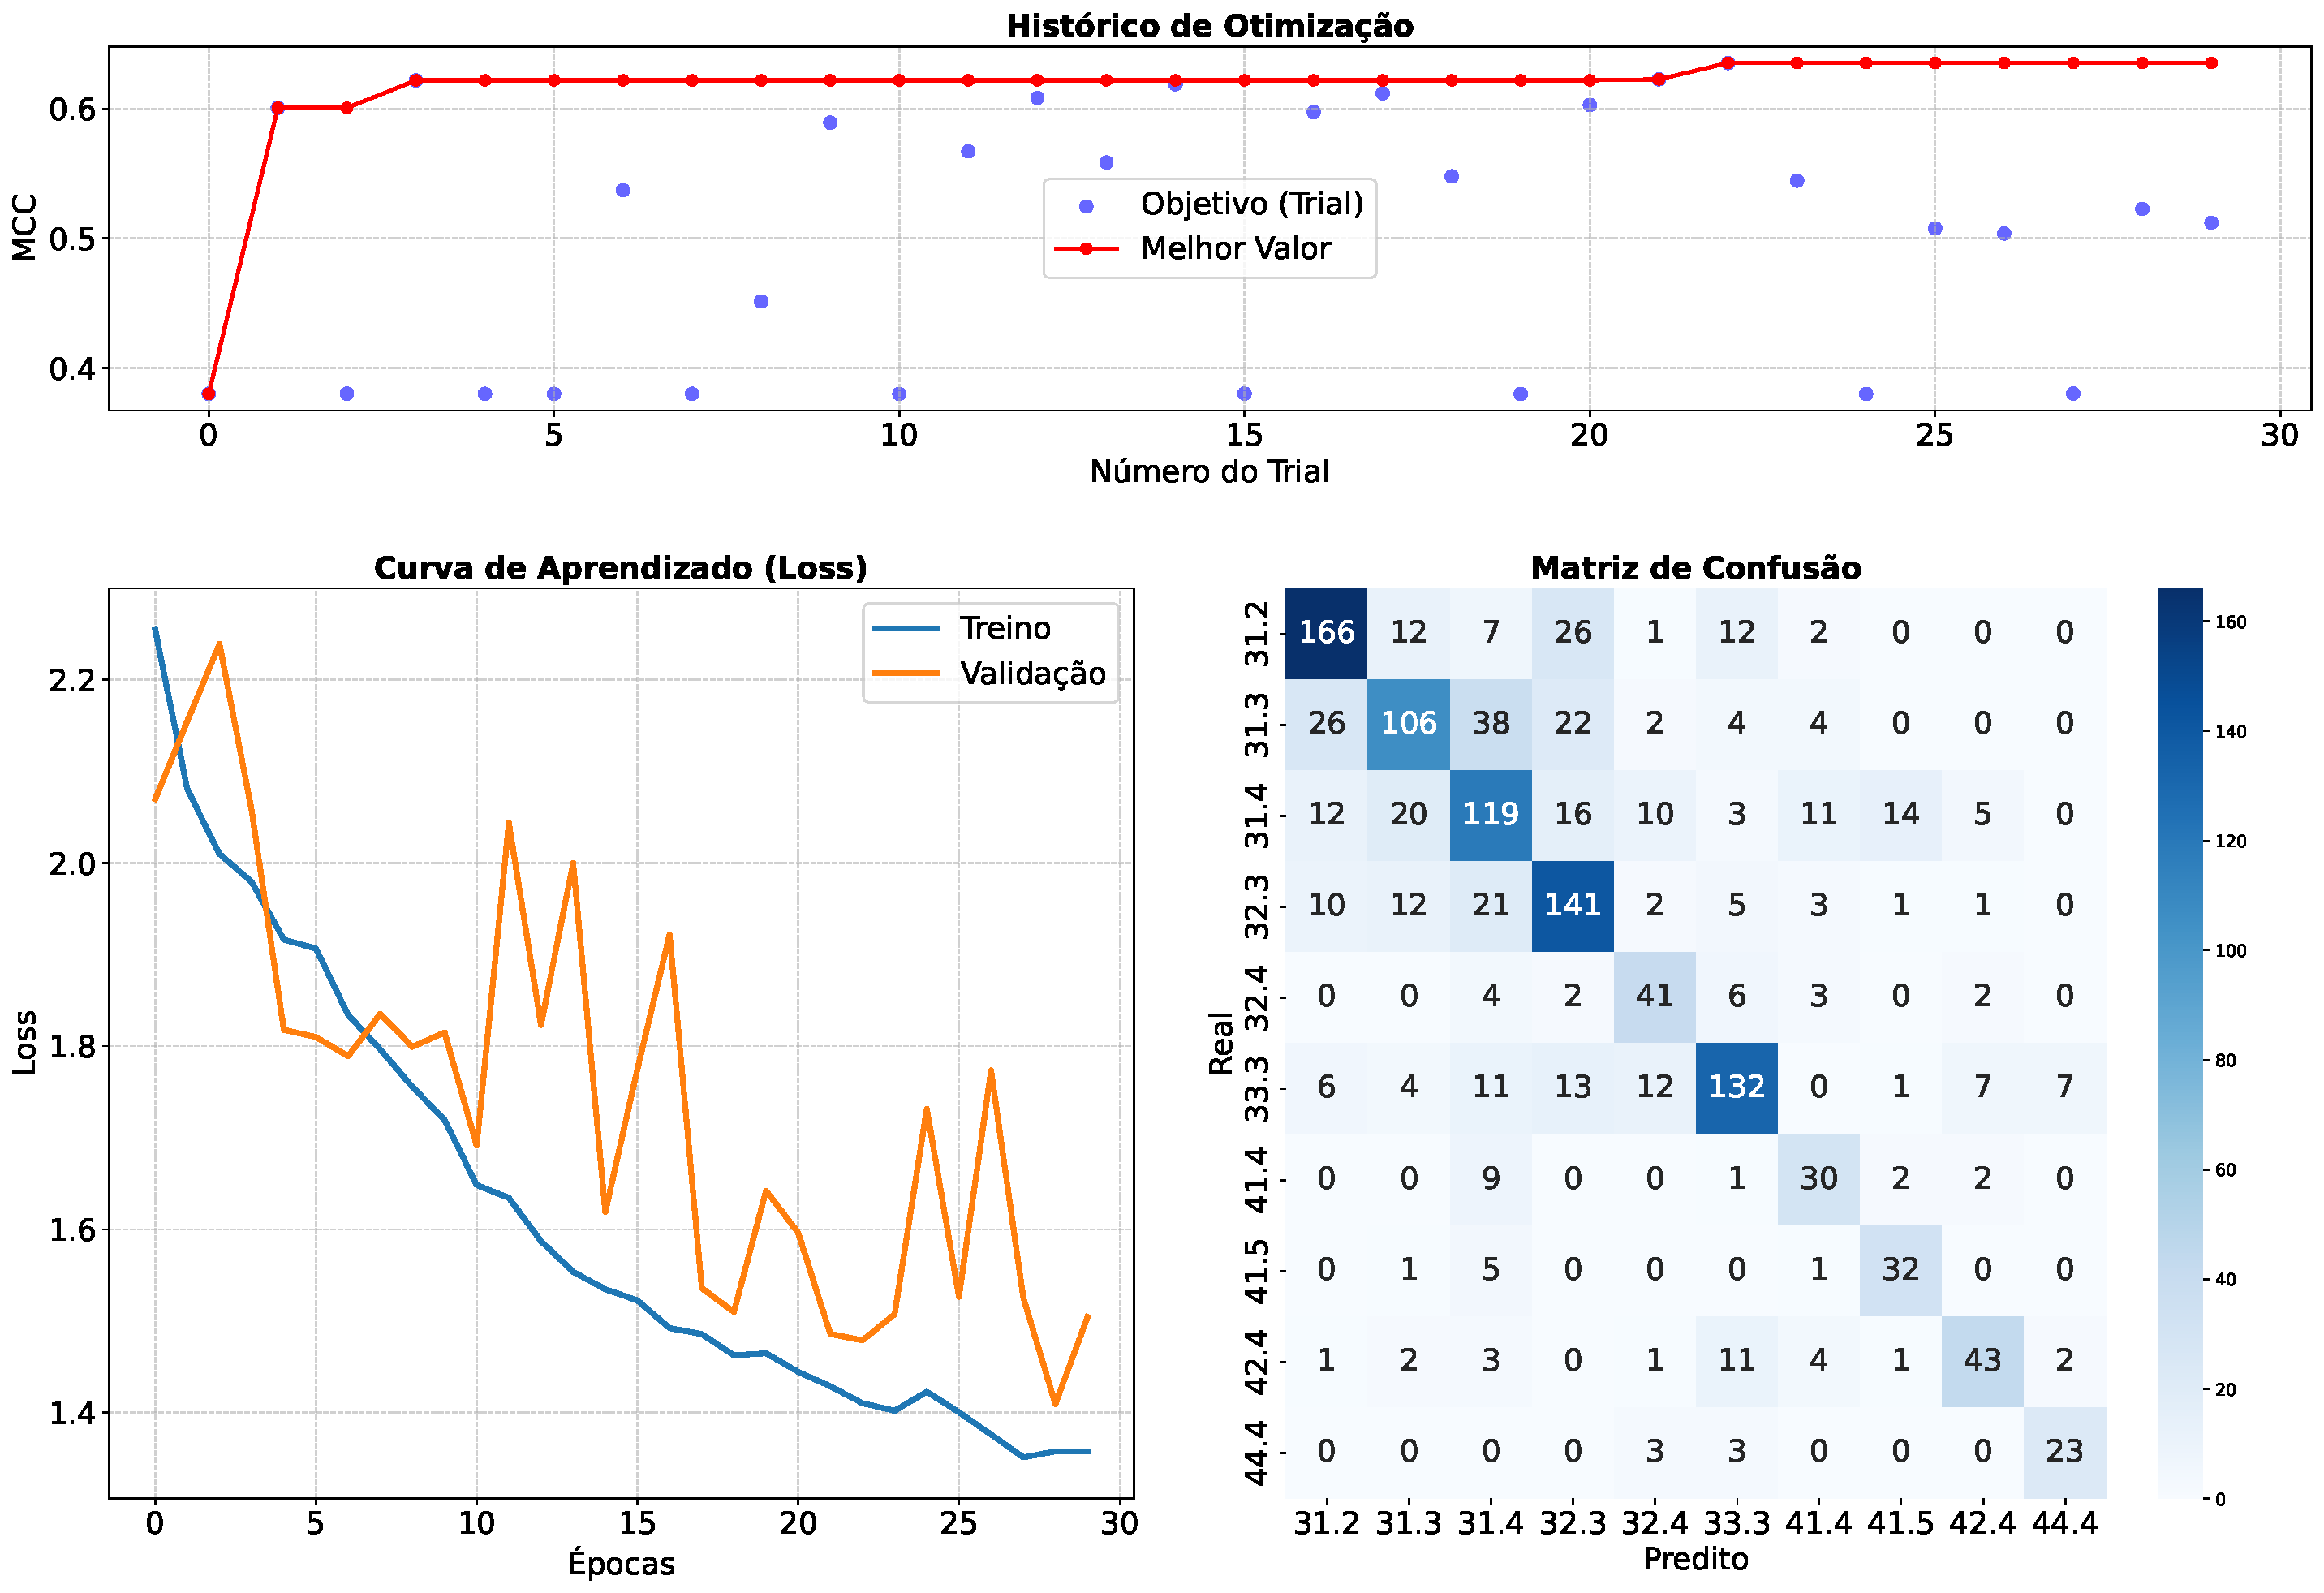
\includegraphics[width=0.85\textwidth]{tex/appendix/experiments/convnext_v1_AB_opt_aug/dashboard_consolidado.pdf}
        \caption{Histórico de Otimização, Curvas de Aprendizado e Matriz de Confusão - convnext\_v1\_AB\_opt\_aug}
    \end{figure}
\end{minipage}
\clearpage


\section*{ConvNeXt V8 AB}
    
\noindent\begin{minipage}{\textwidth}
    \begin{table}[H]
        \centering
        \caption{Hiperparâmetros e Resultados do Melhor Modelo - convnext\_v8\_AB\_opt\_aug}
        \vspace{0.2cm}
        \resizebox{\textwidth}{!}{%
            \begin{tabular}{ll | lrrr}
                \hline
                \multicolumn{2}{c|}{\textbf{Hiperparâmetros}} & \multicolumn{4}{c}{\textbf{Métricas por Classe}} \\ \hline
                \textbf{Parâmetro} & \textbf{Valor} & \textbf{Classe} & \textbf{Precisão} & \textbf{Recall} & \textbf{F1-Score} \\ \hline
    Agendador (Patience) & 3 & 31.2 & 0.4312 & 0.5133 & 0.4687 \\ 
Agendador de LR & ReduceLROnPlateau & 31.3 & 0.2083 & 0.0743 & 0.1095 \\ 
Architecture & convnext\_tiny & 31.4 & 0.1893 & 0.2524 & 0.2163 \\ 
Batch Size & 32 & 32.3 & 0.2078 & 0.3827 & 0.2693 \\ 
Data Augmentation & False & 32.4 & 0.1321 & 0.1207 & 0.1261 \\ 
Decaimento de Peso (WD) & 0.0472 & 33.3 & 0.1854 & 0.1451 & 0.1628 \\ 
Dropout & 0.2874 & 41.4 & 0.1081 & 0.0909 & 0.0988 \\ 
Função de Perda & CrossEntropyLoss & 41.5 & 0.5000 & 0.0513 & 0.0930 \\ 
Hidden Units & 512 & 42.4 & 0.3462 & 0.1324 & 0.1915 \\ 
Label Smoothing & 0.1483 & 44.4 & 0.3333 & 0.1379 & 0.1951 \\ 
\cline{3-6} 
Otimizador & AdamW & \textbf{Média (Macro)} & 0.3077 & 0.1987 & 0.2016 \\ 
Taxa de Aprendizado (LR) & 1.65e-04 & \textbf{MCC} & \multicolumn{3}{c}{0.1353} \\ 
Unfreeze Layers & 6 &  & & &  \\ 
            \hline
            \end{tabular}%
        }
    \end{table}

    \begin{figure}[H]
        \centering
        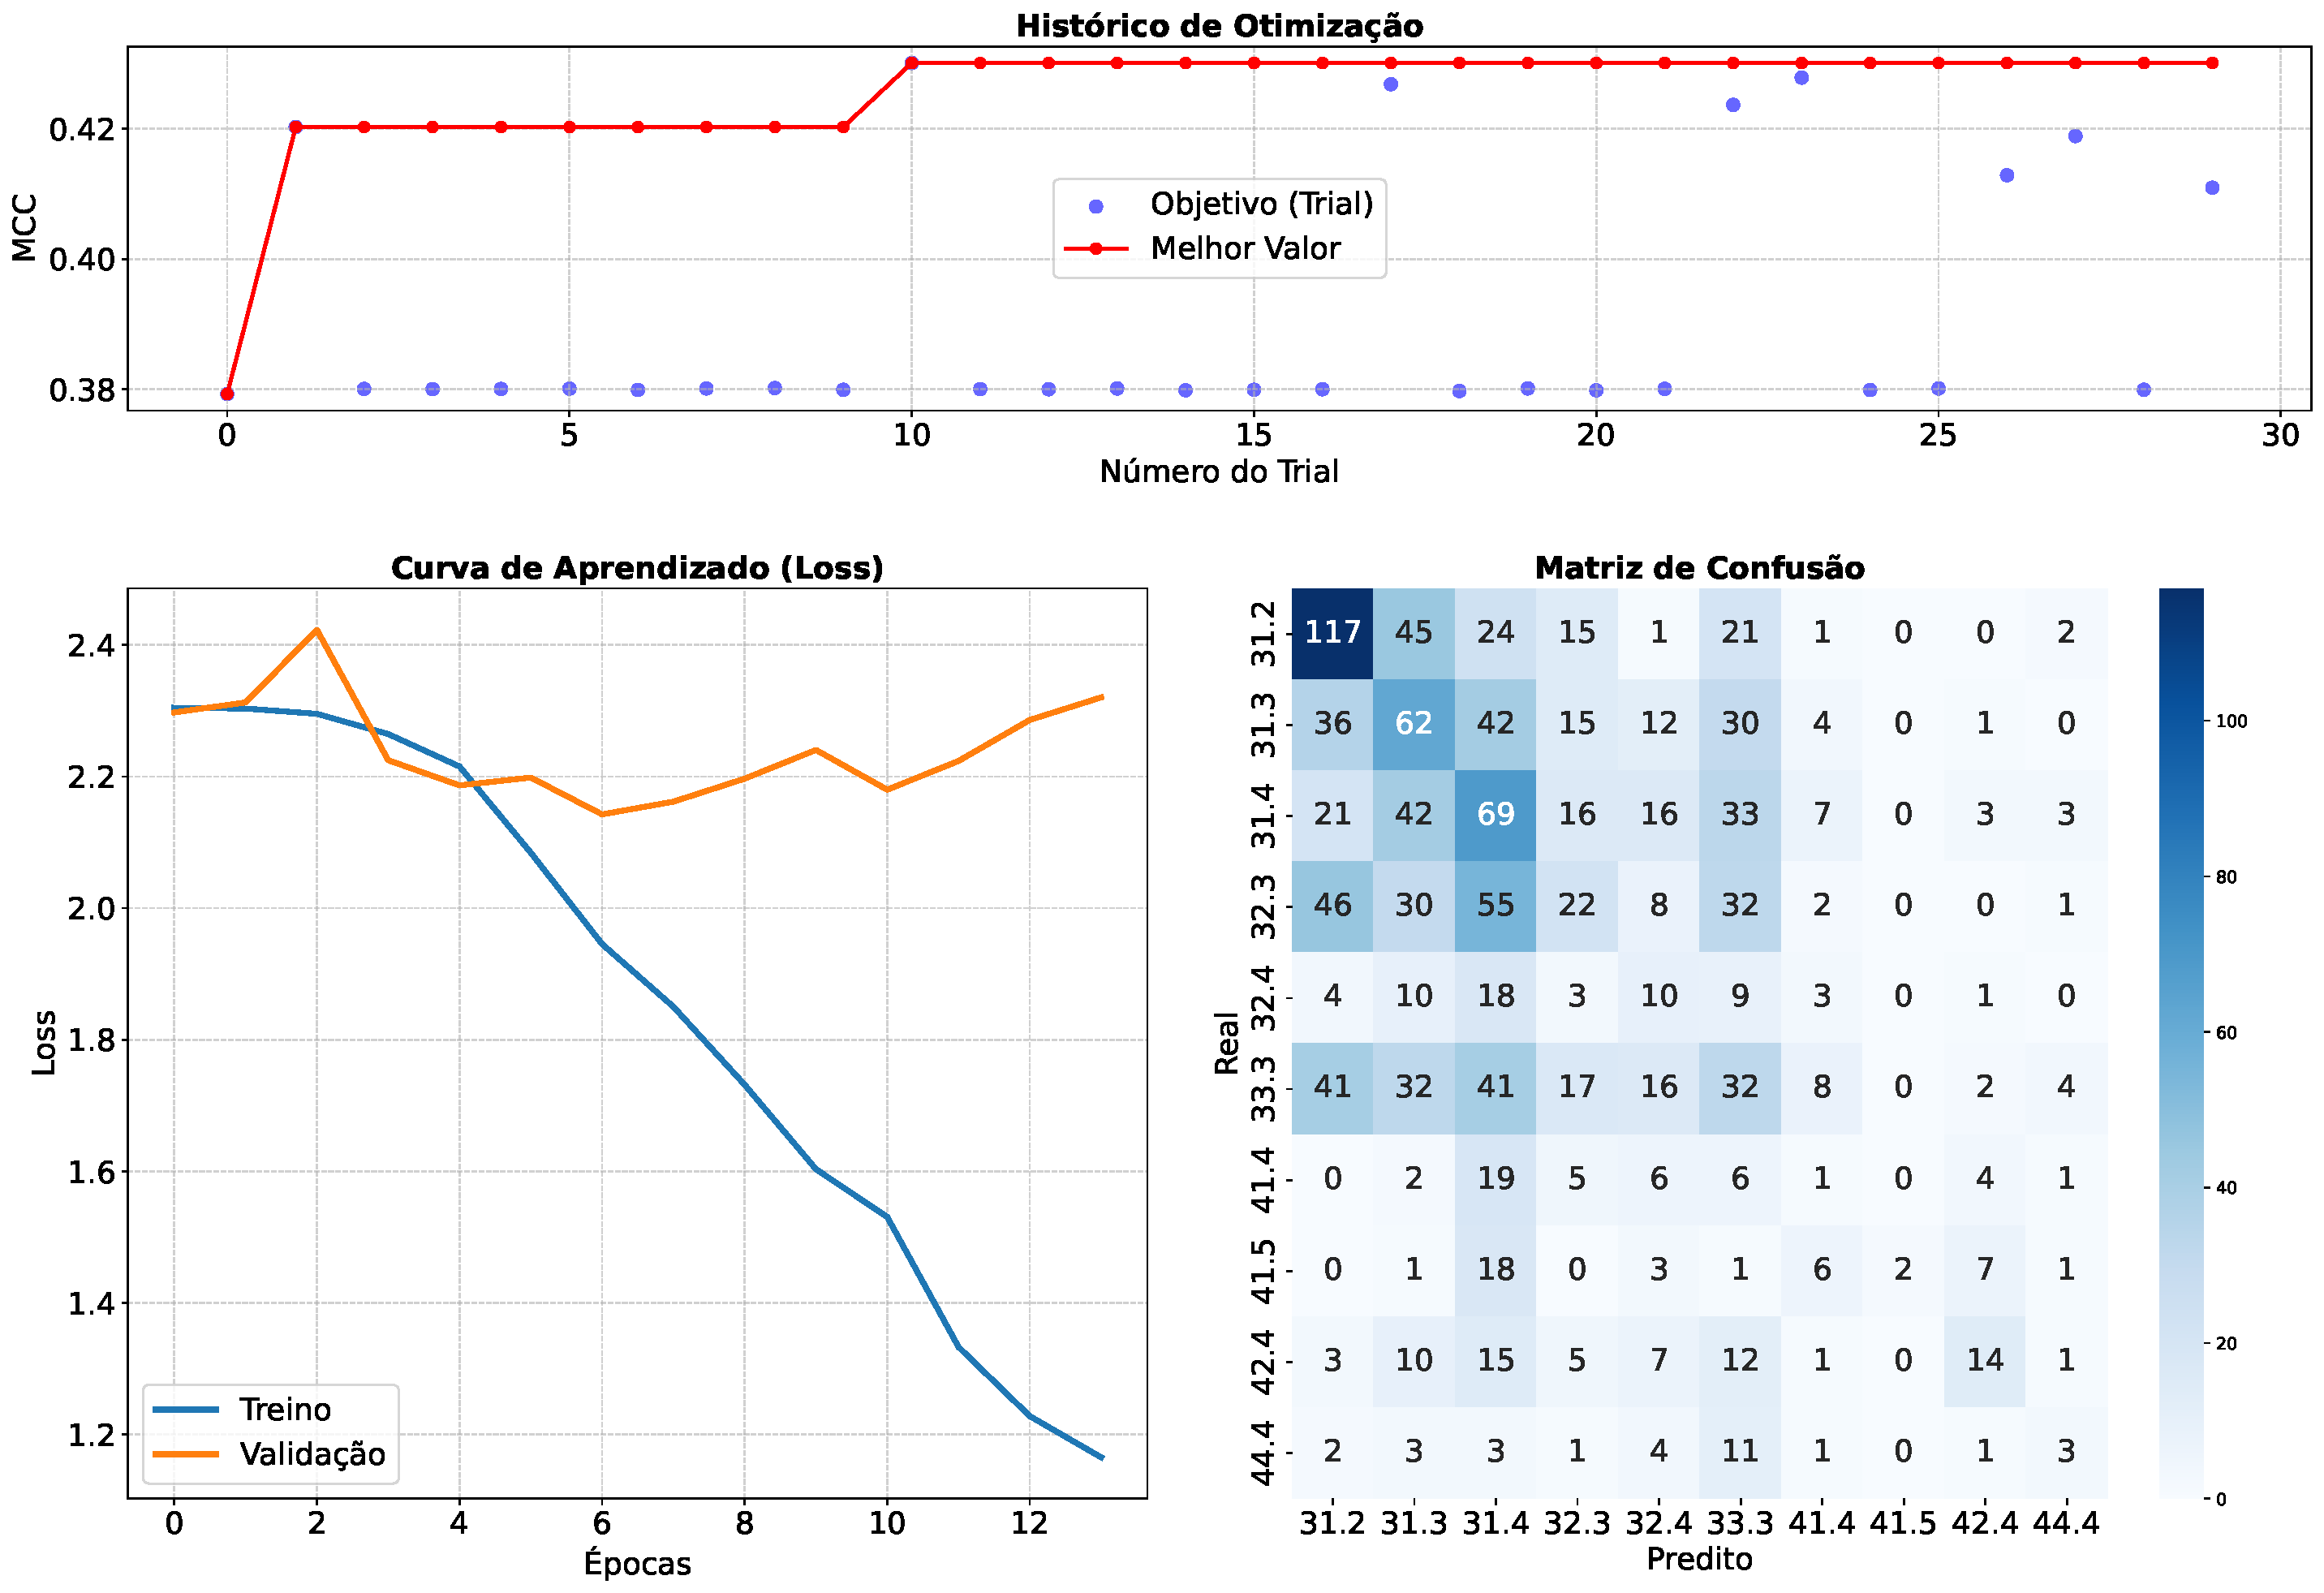
\includegraphics[width=0.85\textwidth]{tex/appendix/experiments/convnext_v8_AB_opt_aug/dashboard_consolidado.pdf}
        \caption{Histórico de Otimização, Curvas de Aprendizado e Matriz de Confusão - convnext\_v8\_AB\_opt\_aug}
    \end{figure}
\end{minipage}
\clearpage


\section*{DenseNet V1 AB}
    \input{tex/appendix/experiments/DenseNet_v1_AB_opt_aug/relatorio_experimento.tex}

\section*{DenseNet V8 AB}
    \input{tex/appendix/experiments/DenseNet_v8_AB_opt_aug/relatorio_experimento.tex}

\section*{EfficientNet V1 AB}
    \input{tex/appendix/experiments/EfficientNet_v1_AB_opt_aug/relatorio_experimento.tex}

\section*{EfficientNet V8 AB}
    \input{tex/appendix/experiments/EfficientNet_v8_AB_opt_aug/relatorio_experimento.tex}

\section*{Inception V1 AB}
    \input{tex/appendix/experiments/Inception_v1_AB_opt_aug/relatorio_experimento.tex}

\section*{Inception V8 AB}
    \input{tex/appendix/experiments/Inception_v8_AB_opt_aug/relatorio_experimento.tex}

\section*{ResNet V1 AB}
    \input{tex/appendix/experiments/ResNet_v1_AB_opt_aug/relatorio_experimento.tex}

\section*{ResNet V8 AB}
    \input{tex/appendix/experiments/ResNet_v8_AB_opt_aug/relatorio_experimento.tex}

\section*{Swin V1 AB}
    \input{tex/appendix/experiments/Swin_v1_AB_opt_aug/relatorio_experimento.tex}

\section*{Swin V8 AB}
    \input{tex/appendix/experiments/Swin_v8_AB_opt_aug/relatorio_experimento.tex}

\section*{VGG V1 AB}
    \input{tex/appendix/experiments/VGG_v1_AB_opt_aug/relatorio_experimento.tex}

\section*{VGG V8 AB}
    \input{tex/appendix/experiments/VGG_v8_AB_opt_aug/relatorio_experimento.tex}

\section*{Vit V1 AB}
    \input{tex/appendix/experiments/Vit_v1_AB_opt_aug/relatorio_experimento.tex}

\section*{Vit V8 AB}
    \input{tex/appendix/experiments/Vit_v8_AB_opt_aug/relatorio_experimento.tex}








\end{apendicesenv}
% ---


% ----------------------------------------------------------
% Anexos
% ----------------------------------------------------------

% ---
% Inicia os anexos
% ---
\begin{anexosenv}

    \chapter{Repositório Git} 
    \label{chapter:pgithub}
    \begin{description}
 \item[\url{https://github.com/rodrigoqaz/mecai.dissertacao}] Repositório com todos os códigos produzidos nesta dissertação;
 \end{description}

\end{anexosenv}
% ---

\end{document}